\documentclass[a4paper, 12pt]{article}

% --- PAQUETES DE IDIOMA Y CODIFICACIÓN ---
\usepackage[utf8]{inputenc}
\usepackage[spanish, es-tabla]{babel} % es-tabla usa "Tabla" en vez de "Cuadro"

% --- PAQUETES DE FORMATO Y DISEÑO ---
\usepackage{graphicx} % Para incluir imágenes
\usepackage{bmpsize}    
\usepackage{caption} % Necesario para el comando \captionof
\usepackage{geometry} % Para márgenes
\usepackage{times}    % Fuente Times New Roman
\usepackage{fancyhdr} % Para encabezados y pies de página
\usepackage{hyperref} % Para enlaces y marcadores en el PDF
\usepackage{url}      % Para formatear URLs correctamente
\usepackage{amsmath} % Imprescindible para entornos de ecuaciones como 'equation'
\usepackage{csvsimple} % Para las tablas csv
\usepackage[table]{xcolor} % Para colorear tablas
\usepackage{booktabs}      % Para líneas horizontales elegantes


\newcommand{\imgpath}{../../source} 

% --- CONFIGURACIÓN DE PÁGINA ---
\setlength{\parskip}{0.3cm} % Espacio entre párrafos

% Configuración de márgenes unificada
\geometry{
 left=2.5cm,
 right=2.5cm,
 top=2.5cm,
 bottom=2.5cm,
 headheight=15pt % Altura necesaria para el encabezado
}

% --- CONFIGURACIÓN DE ENCABEZADO Y PIE ---
\pagestyle{fancy}
\fancyhf{} % Borra los valores por defecto

% Encabezado (L = Izquierda, R = Derecha)
\lhead{\small Práctica Final: Compresión basada en DCT} 
\rhead{\small Compresión Multimedia 25/26} 

% Pie de página (C = Centro -> Número de página)
\cfoot{\thepage}

% Líneas separadoras
\renewcommand{\headrulewidth}{0.4pt} 
\renewcommand{\footrulewidth}{0.4pt} 

% --- INICIO DEL DOCUMENTO ---
\begin{document}

% --- PORTADA ---
\begin{titlepage}
    \centering
    
    % LOGOTIPO
    
\includegraphics[width=0.45\textwidth]{escudo_um.png} 
    
    \vspace{1cm}
    
    {\Large \textbf{Universidad de Murcia}}
    
    \vspace{1cm}
    
    {\large \textsc{Grado en Ingeniería Informática}} \\
    \vspace{0.5cm}
    {\large \textsc{Compresión Multimedia}} \\
    \vspace{0.2cm}
    {\large \textsc{Curso 25/26}}
    
    \vspace{2cm}
    
    {\Huge \textbf{Proyecto Final}} \\
    \vspace{0.5cm}
    {\Large \textsc{Compresión de Imágenes Basada en DCT:}} \\
    \vspace{0.1cm}
    {\Large \textsc{Estudio Experimental}}
    
    \vspace{2cm}
    
    % DATOS DEL ALUMNO
    {\large \textbf{Jorge Serrano Rueda}} \\
    \vspace{0.1cm}
    \texttt{jorge.serranor@um.es} \\
    \vspace{0.5cm}
    \textbf{Grupo: 1.1}
    
    \vfill
    
    % PROFESOR Y FECHA
    Profesor: Nespoli, Pantaleone \\
    \vspace{1cm}
    14 de diciembre de 2025
    
\end{titlepage}

% --- ÍNDICES ---
\newpage
\listoffigures 
\tableofcontents

% --- RESUMEN ---
\newpage 
\pagenumbering{arabic} % Reinicia contador a 1

\section{Resumen}

El presente documento recoge el trabajo desarrollado en el marco de las prácticas de la asignatura Compresión Multimedia (convocatoria de enero, curso 2025/2026). El núcleo del proyecto consiste en la implementación y evaluación de dos sistemas de compresión de imágenes fundamentados en la Transformada Discreta del Coseno (DCT) y la codificación Huffman.

La estructura del informe abarca desde los fundamentos teóricos y la descripción detallada de la metodología experimental, hasta un exhaustivo análisis de los datos obtenidos, abordando tanto la perspectiva cualitativa como la cuantitativa. Finalmente, se presentan las conclusiones derivadas del estudio. El objetivo principal es contrastar el rendimiento de ambos compresores, identificando las variables que impactan en su eficacia para determinar las condiciones y configuraciones óptimas que garanticen los mejores resultados de forma generalizada.

% --- INTRODUCCIÓN ---
\newpage 
\section{Introducción}

En el panorama tecnológico actual, la compresión de imágenes se ha erigido como un pilar indispensable, abarcando desde aplicaciones científicas avanzadas hasta las interacciones digitales cotidianas. La era digital ha traído consigo una producción y consumo masivo de contenidos visuales sin precedentes, planteando retos significativos en términos de almacenamiento y ancho de banda.

La necesidad de transmitir datos de manera eficiente se hace evidente en escenarios críticos: desde el envío de fotografías en redes con conectividad limitada hasta el intercambio de imaginería médica de alta resolución, donde preservar la integridad del detalle es vital. En este contexto, los algoritmos de compresión son la herramienta clave para reducir el peso de los archivos garantizando la viabilidad de su transmisión.

Fundamentado en la Teoría de la Información, este proyecto implementa codificadores basados en el algoritmo de Huffman en dos variantes. Paralelamente, se integra la Transformada Discreta del Coseno (DCT) que, en conjunción con procesos de cuantización, permite optimizar la tasa de compresión manteniendo una calidad visual aceptable. La combinación de estas técnicas permite una aproximación funcional al estándar JPEG. Mediante una metodología experimental rigurosa sobre un banco de imágenes específico, se evaluará el rendimiento, los límites operativos y los escenarios de uso óptimo para estas estrategias de compresión.

Los resultados esperables del proyecto incluyen una reducción significativa del tamaño de las imágenes, manteniendo una calidad visual aceptable perceptible para el ojo humano. La combinación de la Transformada Discreta del Coseno y la codificación Huffman permite comprimir archivos BMP grandes en versiones mucho más ligeras, optimizando almacenamiento y transmisión. Además, se podrá evaluar cuantitativamente el rendimiento mediante métricas como la relación de compresión y el error promedio.

% --- METODOLOGÍA ---
\newpage
\section{Metodología}

\subsection{Compresores Desarrollados y Principios de Compresión \textit{Lossy}}

Para el desarrollo de esta práctica se han implementado dos compresores de imagen que emplean un esquema de \textbf{compresión con pérdida} (\textit{lossy}), basado en los principios del estándar \textbf{JPEG} (ITU T.81). Ambos compresores siguen una secuencia de tres pasos clave: Transformada, Cuantificación y Codificación.

\subsection{Proceso de Compresión}

Partimos de una imagen definida por un número determinado de filas y columnas, cuya unidad básica es el píxel. El objetivo es transformar esa representación en una forma equivalente que permita describir el contenido visual de manera más compacta y facilitar la aplicación de operaciones posteriores.

\subsubsection{Conversión del espacio de color}
Existen distintas formas de representar los colores y los píxeles de una imagen, entre ellas las tablas indexadas, el espacio RGB, el espacio YCbCr, entre otros. Sin embargo, dado que el ojo humano es más sensible a los cambios de \textbf{luminancia} que a los de \textbf{crominancia}, se aplica una conversión desde RGB al espacio \textbf{YCbCr}. Este espacio separa la información de brillo (Y) de la información de color (Cb y Cr), lo que permite optimizar el proceso de compresión ajustándolo mejor a la forma en que el ser humano percibe los colores.


\begin{center}
    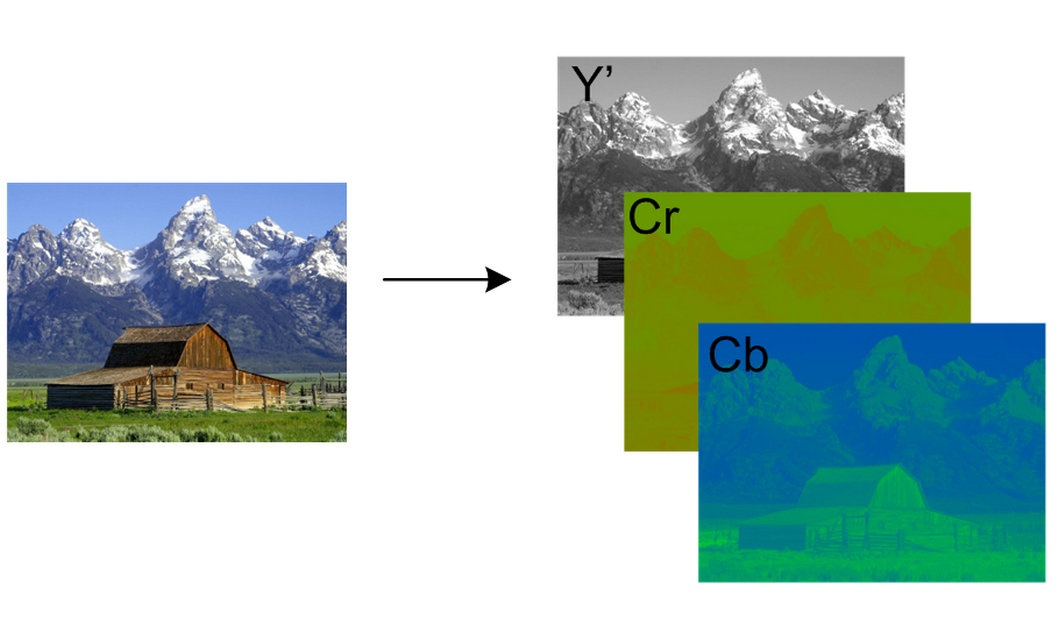
\includegraphics[width=0.7\textwidth]{./Images/YCbCr.jpg}
\end{center}

\subsubsection{Transformada Discreta del Coseno (DCT)}
Una vez obtenida la imagen en el espacio YCbCr, el primer paso consiste en dividirla en bloques de $8 \times 8$ píxeles. Si las dimensiones de la imagen no son múltiplo de $8$, se amplían duplicando las últimas filas o columnas para completar el bloque, y posteriormente se restauran al finalizar la compresión.

A cada bloque se le aplica la \textbf{Transformada Discreta del Coseno} (DCT). Su función principal es \textbf{decorrelacionar} y concentrar la energía de los datos. 

En términos sencillos, decorrelacionar significa separar o “desmezclar” la información que está distribuida de forma redundante en los píxeles, convirtiendo el bloque en un conjunto de valores más independientes entre sí. Por otro lado, \textbf{compactar la energía} implica reorganizar la información del bloque de manera que la mayor parte de los detalles importantes se acumulen en unos pocos coeficientes (las bajas frecuencias), mientras que los coeficientes restantes contienen cambios menores o poco relevantes visualmente.  

La aplicación de la DCT permite expresar cada bloque de $8 \times 8$ píxeles como una \textbf{combinación lineal de 64 patrones básicos}, conocidos como \textit{bases de frecuencia}. Cada uno de estos patrones corresponde a un coeficiente de la DCT, que indica cuánto contribuye ese patrón al bloque original. En otras palabras, cualquier bloque de imagen puede reconstruirse sumando estos 64 patrones, cada uno escalado por su coeficiente correspondiente. Este es precisamente el motivo por el que aplicamos la transformada:

La mayor parte de la información visual significativa (las bajas frecuencias) se concentra en los \textbf{coeficientes DC} y las primeras componentes \textbf{AC}. El coeficiente \textbf{DC} representa el valor promedio del bloque, mientras que los coeficientes \textbf{AC} representan las variaciones respecto al valor promedio, es decir, los detalles y texturas de la imagen. Los coeficientes de alta frecuencia (AC más alejados del DC) tienden a aproximarse a cero, ya que representan detalles finos o ruido, lo cual es crucial para reducir el tamaño de la imagen.  

% Imagen zigzag
\begin{center}
    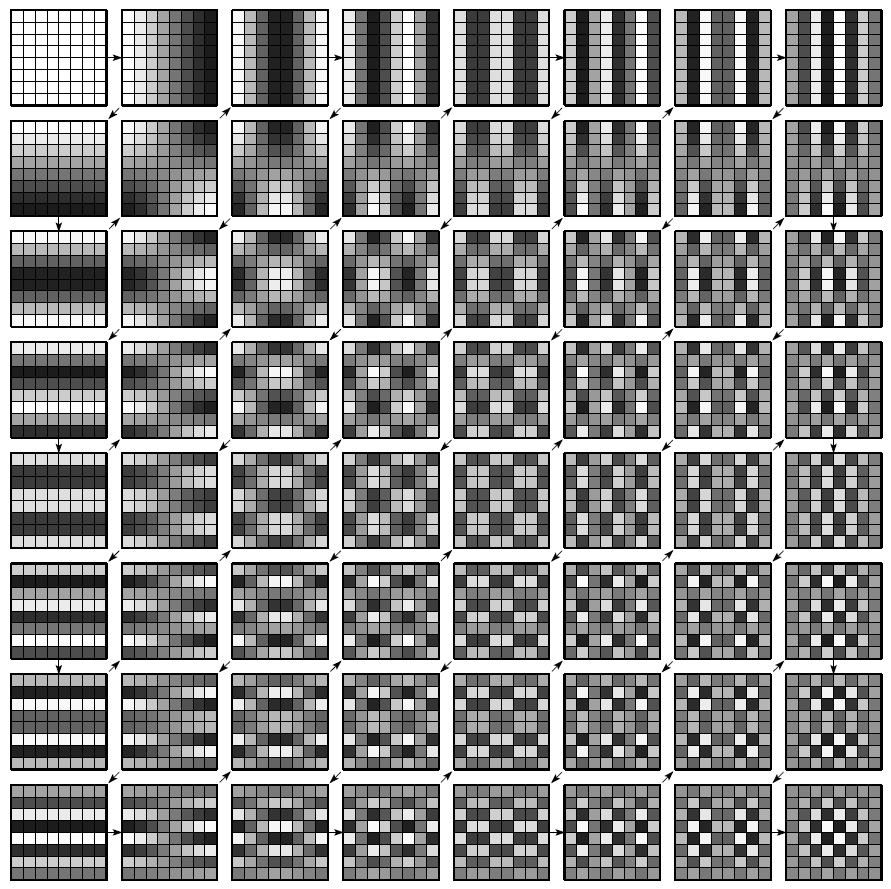
\includegraphics[width=0.5\textwidth]{./Images/DCT_2D.png}
    \captionof{figure}{Bases de la DCT.}
\end{center}
\vspace{0.5cm}

Para mejorar la eficiencia en los pasos posteriores, como la cuantificación y la codificación, se suele reordenar los coeficientes del bloque siguiendo un \textbf{orden en zigzag}. Este orden permite que los coeficientes más relevantes (DC y primeras AC) queden en las primeras posiciones, agrupando los coeficientes cercanos a cero hacia el final del bloque. Esto facilita la compresión, ya que los valores pequeños pueden ser más fácilmente codificados de manera eficiente.  

% Imagen zigzag
\begin{center}
    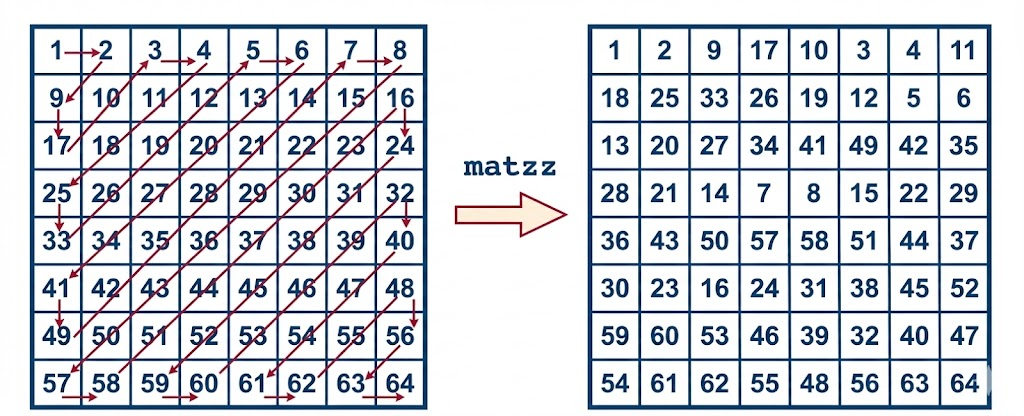
\includegraphics[width=1\textwidth]{./zigzag.jpg}
    \captionof{figure}{Reordenación en zigzag.}
\end{center}
\vspace{0.5cm}


\subsubsection{Cuantificación y el Factor CaliQ (Introducción de Pérdida)}
La cuantificación es el paso donde se introduce la pérdida de información y se logra la compresión principal. Su \textbf{finalidad} es reducir la precisión con la que se almacenan los coeficientes de la DCT, aprovechando las limitaciones del sistema visual humano. Los coeficientes de alta frecuencia (que contienen detalles finos) suelen tener menor impacto y son menos perceptibles; por lo tanto, la cuantificación los descarta o los almacena con mucha menos precisión que los coeficientes de baja frecuencia (que contienen el brillo y contraste general).

\begin{itemize}
    \item Los coeficientes de frecuencia de la DCT son \textbf{divididos} por una matriz de pesos extraídos de las \textbf{Tablas de Cuantificación} recomendadas en el estándar \textbf{ITU T.81} (el estándar JPEG).
    \item Se utiliza un parámetro de escalado, denominado \textbf{CaliQ} (Calidad de Cuantificación), para \textbf{multiplicar} cada valor de la tabla ITU T.81, controlando directamente el nivel de pérdida.
\end{itemize}

La operación de cuantificación se define como:
\begin{equation}
\text{Coeficiente Cuantificado} = \text{round}\left( \frac{\text{Coeficiente DCT}}{\text{Valor de Tabla ITU T.81} \times \text{CaliQ}} \right)
\end{equation}

Al realizar la división, muchos coeficientes (especialmente los de alta frecuencia) se redondean a cero. Esta reducción de datos crea largas secuencias de ceros que son posteriormente comprimidas de manera muy eficiente en la etapa de codificación entrópica.

Un valor de \textbf{CaliQ más alto} implica un divisor mayor. Esto resulta en que una mayor cantidad de coeficientes de frecuencia, especialmente aquellos que contienen poca energía, se \textbf{redondeen a cero} (proceso de truncamiento). Este paso busca \textbf{maximizar la anulación de coeficientes}, lo que reduce significativamente la cantidad de datos a codificar. Cuanto mayor sea CaliQ, mayor debe ser la \textbf{magnitud} (consideramos que los coeficientes con mayor magnitud son los que transportan mayor información) de un coeficiente original para que no sea anulado.

\paragraph{Tipos de Cuantificación}
Existen diversos enfoques para la cuantificación. El método principal utilizado en este proyecto es la \textbf{cuantificación uniforme} dependiente de la frecuencia, donde cada coeficiente se trata de manera distinta según su posición. Alternativamente, estudiaremos otros métodos como:

\begin{itemize}
    \item \textbf{Cuantificación Zonal (Codificación Zonal):} Consiste en descartar todos los coeficientes que se encuentran fuera de una zona predefinida del bloque DCT (ej. solo conservar los coeficientes de menor frecuencia). Es una simplificación estricta que es menos flexible.
    \item \textbf{Cuantificación por Umbral (Thresholding):} Se descartan todos los coeficientes cuyo valor absoluto es inferior a un umbral predefinido. Es un método que se enfoca en la energía, independientemente de la frecuencia.
\end{itemize}

Como la cuantificación introduce pérdidas, la calidad visual de la imagen resultante será inversamente proporcional al factor $\text{CaliQ}$ utilizado. La calidad se medirá mediante métricas objetivas como los \textbf{bits medios por píxel (BPP)} y el \textbf{Error Cuadrático Medio (MSE)}, las cuales se detallarán posteriormente.

\subsubsection{Codificación Entrópica (Algoritmo Huffman)}
Finalmente, los coeficientes cuantificados se codifican utilizando el algoritmo de \textbf{Huffman}. Este es un método de codificación de longitud variable que optimiza la compresión asignando códigos binarios más cortos a los valores (palabras) que ocurren con mayor frecuencia y códigos más largos a los menos frecuentes. La eficiencia de este paso depende de los coeficientes cuantificados.

En el contexto de la compresión con Huffman, una \textbf{tabla Huffman} permite codificar símbolos de manera eficiente asignando códigos de longitud variable según la frecuencia de aparición de cada símbolo. Esta tabla se organiza usando varias estructuras clave:

\begin{itemize}
    \item \textbf{MINCODE:} Contiene el valor numérico más pequeño de los códigos para cada longitud de bits $L$. Sirve para determinar el rango mínimo de códigos de esa longitud.
    
    \item \textbf{MAXCODE:} Contiene el valor numérico más grande de los códigos para cada longitud $L$. Si un código leído es menor o igual a este valor, significa que se ha leído completamente un código válido.
    
    \item \textbf{VALPTR:} Es un índice o puntero que indica dónde comienza la lista de símbolos correspondientes a esa longitud de código dentro de la tabla de símbolos (HUFFVAL). Permite localizar rápidamente qué símbolo corresponde a un código leído.
\end{itemize}


\textbf{Nota:} Definimos la Información Lateral como el conjunto de datos auxiliares que, si bien no pertenecen intrínsecamente a la imagen original, son generados durante la ejecución completa del proceso (por ejemplo, durante la codificación, compresión o transmisión) y son necesarios para el correcto funcionamiento. 
 
\subsubsection{Diferenciación de Compresores}

La diferencia fundamental entre los dos compresores reside en la implementación y el uso de las tablas del algoritmo de Huffman:

\begin{itemize}
    \item \textbf{Compresor Default:}
    Este compresor utiliza las tablas Huffman predeterminadas especificadas en el estándar ITU T.81 (JPEG). Estas tablas están diseñadas para un ámbito general de imágenes, pero no son óptimas para los valores de las frecuencias específicas de la imagen procesada.

    \item \textbf{Compresor Custom:}
    Este compresor calcula tablas Huffman específicas para cada imagen. Analiza la frecuencia real de aparición de cada coeficiente cuantificado y genera un conjunto de códigos que están optimamente ajustados a esa distribución de datos particular. Por lo tanto, se espera que este compresor logre resultados mejores o similares de compresión que el compresor \textit{Default} para un mismo factor $\text{CaliQ}$.
\end{itemize}

\subsubsection{Proceso Inverso (Reconstrucción)}

La reconstrucción de la imagen comprimida consiste en aplicar los pasos inversos del proceso de compresión, intentando recuperar la mayor similitud posible con la imagen original. Primero, se realiza la \textbf{decodificación Huffman} para recuperar los coeficientes cuantificados de cada bloque. Luego, se aplica la \textbf{descuantificación}, multiplicando cada coeficiente por los valores de la tabla de cuantificación y el factor $\text{CaliQ}$ correspondiente. Posteriormente, se ejecuta la \textbf{Transformada Discreta del Coseno inversa (IDCT)} sobre cada bloque, reconstruyendo los valores de píxeles aproximados en el espacio YCbCr. Finalmente, se realiza la \textbf{conversión inversa a RGB} para obtener la imagen final en su formato original.


\subsection{Datos de entrada}
\subsubsection{Formato de los datos}
Los datos de entrada para el análisis experimental han sido imágenes Truecolor con formato BMP, otros formatos con compresión sin pedidas también podrían ser validos. En caso de que se usen formato con perdidas las métricas utilizas y datos obtenidos no tendrían interés experimental.

\subsubsection{Valores elegidos para CaliQ}
Respecto a los factores elegidos, utilizamos los siguientes valores:

\[
[5, 25, 50, 100, 200, 400, 800, 1600]
\]
 
\textbf{Nota:} Los valores inferiores a 100 producirán una salida con mayor calidad que la del estándar jpeg.

Con el objetivo de explorar dos aspectos principales: primero, identificar el punto óptimo entre la compresión y la preservación de la calidad visual; y segundo, analizar los principios y límites del compresor, determinando en qué casos el factor \texttt{caliQ} resulta insignificante.


\subsection{Método de evaluación}
En este estudio se realizan dos análisis de los resultados obtenidos:
\begin{itemize}
    \item  \textbf{Cualitativo:} Se analiza desde un punto de vista visual, tenemos en cuenta como de notorios son los cambios introducidos por el proceso de cuantificación. Catalogaremos los resultados objetivamente analizando la aparición de artefactos visuales y valorando la similitud entre las imágenes reconstruidas y las originales.
    \item   \textbf{Cuantitativo:} Se analiza a nivel teórico y técnico los resultados obtenidos utilizando métricas. 
\end{itemize}

\subsubsection{Artefactos de Imagen}

Un \textbf{artefacto de imagen} es cualquier falla, distorsión o imperfección visual no deseada que aparece en una imagen digital y que no estaba presente en la imagen original. Estos artefactos se original durante el proceso de cuantificación.


\begin{itemize}
    \item \textbf{Banding (Bandas de color / Posterización)}  
    Aparición de escalones visibles en regiones que deberían mostrar transiciones suaves de color (cielos, sombras).  
    Se produce por falta de resolución tonal (profundidad de color baja) o por una compresión excesiva.

    \begin{center}
    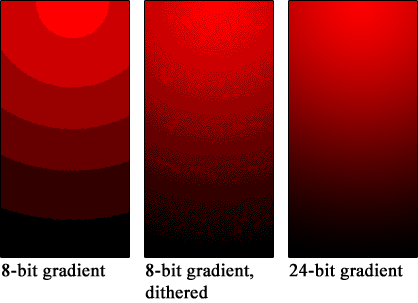
\includegraphics[width=0.4 \textwidth]{./Images/banding.png}
    \captionof{figure}{Ejemplo visual del artefacto Banding.}
    \end{center}

    \item \textbf{Blocking (Bloqueo / Macroblocking)}  
    Aparición de bloques perceptibles, normalmente de $8 \times 8$ o $16 \times 16$ píxeles.  
    Es característico de la compresión JPEG agresiva, donde el procesamiento por bloques deja de ser imperceptible.

    \begin{center}
    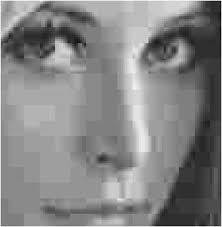
\includegraphics[width=0.3 \textwidth]{./Images/bloking.jpeg}
    \captionof{figure}{Ejemplo visual del artefacto Blocking.}
    \end{center}

    \item \textbf{Ringing (Efecto halo / Timbre)}  
    Presencia de halos o pequeñas oscilaciones alrededor de bordes de alto contraste.  
    Se origina por compresión fuerte o por filtrado de \emph{sharpening} aplicado de forma excesiva.

    \begin{center}
    
\includegraphics[width=0.4 \textwidth]{./Images/Ringing_artifact.png}
    \captionof{figure}{Ejemplo visual del artefacto Ringing.}
    \end{center}

    \item El \textbf{Aliasing} es un efecto que aparece cuando una imagen se representa con una resolución insuficiente. 
    Esto provoca artefactos visuales como bordes dentados o patrones falsos, ya que los detalles finos no se
    capturan correctamente.

        \begin{center}
    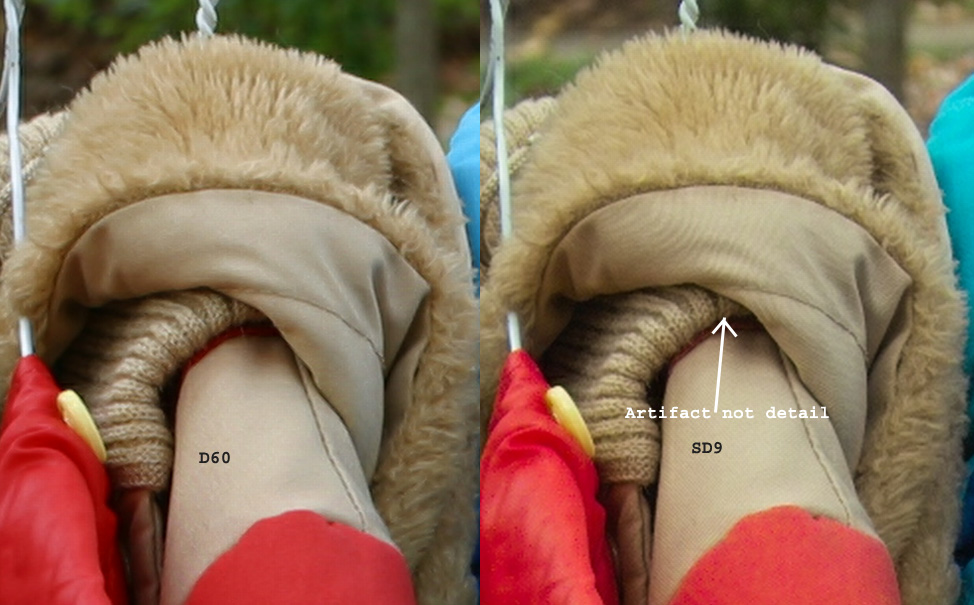
\includegraphics[width=0.4 \textwidth]{./Images/artifact.jpg}
    \captionof{figure}{Ejemplo visual del artefacto Aliasing.}
    \end{center}

    \item \textbf{Ruido (Noise)}  
    Variaciones aleatorias de luminancia o color que generan una apariencia granulada. Es habitual en condiciones de poca luz o valores ISO altos.

    \item \textbf{Pixelación}  
    Los píxeles se vuelven visibles al ampliar en exceso una imagen de baja resolución, provocando una apariencia en bloques.
\end{itemize}


\subsubsection{Métricas de evaluación}

\textbf{Error Cuadrático Medio (MSE)} es el error introducido por el cuantificador y mide la distancia promedio entre cada valor original de la imagen y el valor correspondiente en la imagen recuperada, es una medida de fidelidad.


\begin{equation}
\text{MSE} = \frac{1}{N} \sum_{i=1}^{N} \left( x_{i} - Q(x_{i}) \right)^2
\end{equation}

\begin{itemize}
    \item[$N$] \textbf{Número Total de Coeficientes} (o píxeles) evaluados en la imagen o en el bloque.
    \item[$\sum_{i=1}^{N}$] \textbf{Sumatoria}. Indica la suma de los errores al cuadrado para todos los coeficientes desde $i=1$ hasta $N$.
    \item[$x_{i}$] \textbf{Coeficiente Original} en la posición $i$.
    \item[$Q(x_{i})$] \textbf{Coeficiente Cuantificado} en la posición $i$ (el valor que introduce la pérdida).
\end{itemize}
\vspace{0.5cm}

\textbf{Tasa de Compresión (RC \%)} indica qué porcentaje del tamaño original del fichero se ha reducido (eliminado) después de la compresión.


\begin{equation}
\text{RC (\%)} = \frac{T_{i} - T_{o}}{T_{i}} \times 100
\end{equation}

\begin{itemize}
    \item[$T_{i}$] \textbf{Tamaño de la Fuente Inicial} (o tamaño del archivo original).
    \item[$T_{o}$] \textbf{Tamaño del Archivo Comprimido} (o tamaño de salida).
\end{itemize}
\vspace{0.5cm}

$\text{SNR}(dB)$ \textbf{Relación Señal a Ruido} (\textit{Signal-to-Noise Ratio}). Métrica que compara el nivel de potencia de la señal con el nivel del ruido de fondo, expresada en decibelios (dB).

\begin{equation}
\text{SNR}(dB) = 10 \cdot \log_{10} \frac{\sigma_{s}^{2}}{\sigma_{q}^{2}} = 20 \cdot \log_{10} \frac{\sigma_{s}}{\sigma_{q}}
\end{equation}

\begin{itemize}
    \item[$\sigma_{s}^{2}$] \textbf{Varianza de la Señal} (Potencia de la Señal). Representa la potencia de la señal original o de los coeficientes DCT.
    \item[$\sigma_{q}^{2}$] \textbf{Varianza del Ruido de Cuantificación} (Potencia del Ruido). Representa la potencia del error o distorsión introducida por el proceso de cuantificación.
\end{itemize}
\vspace{0.5cm}

% \begin{equation}
% \text{SSIM}(x, y) = [l(x, y)]^{\alpha} \cdot [c(x, y)]^{\beta} \cdot [s(x, y)]^{\gamma}
% \end{equation}

% \begin{itemize}
%     \item[$\text{SSIM}(x, y)$] \textbf{Índice de Similitud Estructural} entre la ventana de la imagen original ($x$) y la ventana de la imagen recuperada ($y$). El valor está en el rango $[0, 1]$, donde $1$ indica identidad perfecta.
%     \item[$\mu_{x}$ y $\mu_{y}$] \textbf{Media} de los valores de píxel en la ventana $x$ y $y$, respectivamente (comparación de \textbf{Luminancia}).
%     \item[$\sigma_{x}^{2}$ y $\sigma_{y}^{2}$] \textbf{Varianza} de los valores de píxel en $x$ y $y$, respectivamente. La raíz cuadrada ($\sigma$) es la desviación estándar (comparación de \textbf{Contraste}).
%     \item[$\sigma_{xy}$] \textbf{Covarianza} entre $x$ e $y$ (comparación de \textbf{Estructura}).
%     \item[$C_{1}, C_{2}, C_{3}$] \textbf{Constantes pequeñas} para evitar inestabilidad cuando los denominadores son muy cercanos a cero. Se definen usualmente como $C_1 = (K_1 L)^2$ y $C_2 = (K_2 L)^2$, donde $L$ es el rango dinámico de los píxeles (ej: 255 para 8-bit) y $K_1, K_2$ son constantes pequeñas (ej: $0.01$ y $0.03$). $C_3 = C_2 / 2$.
% \end{itemize}


\subsection{Procedimiento experimental y software}
La metodología seguida para la realización del estudio ha sido simple pero efectiva, garantizando la sistematicidad y la trazabilidad de los datos. Primero se desarrolló un fichero \textbf{benchmark} para automatizar la generación de imágenes, gráficos, tablas y otros recursos. Una vez finalizado este paso, se realizó una elección de imágenes. Elegidos los datos experimentales, se formuló una \textbf{hipótesis} sobre los resultados esperables para cada una de ellas, para finalmente ejecutar las pruebas y tests, generando los gráficos y tablas necesarios para el análisis.
\subsubsection{Versión de MATLAB}
Con el fin de asegurar la replicabilidad de los resultados, se empleó MATLAB R2020b, accesible a través de los escritorios virtuales (EVA).
\subsubsection{Software Desarrollado}
Para garantizar la uniformidad y eficiencia del experimento, se implementó un script principal de automatización, denominado benchmark, cuya función fue gestionar el flujo de trabajo:

\begin{itemize}
    \item \textbf{Flujo:} El sistema recorre automáticamente el conjunto de imágenes seleccionadas y aplica la totalidad de los factores de calidad ($Q$) definidos. Esta metodología responde a la pregunta de cómo se obtuvieron los datos necesarios para trazar las curvas de rendimiento.
    
    \item \textbf{Obtención:} En cada iteración (Imagen $\times$ Factor $CaliQ$), el marco ejecuta las funciones de descompresión y recopila las métricas clave: Relación de Compresión (RC), Error Cuadrático Medio (MSE) y SNR.
    
    \item \textbf{Gestión de datos:} Una vez completada la batería de pruebas, el software organiza los datos en una estructura unificada y emplea funciones específicas para:
    \begin{itemize}
        \item \textbf{Generar Gráficas:} Generar los gráficos de rendimiento, como las curvas de RC versus MSE.
        \item \textbf{Generar Tablas:} Crear tablas de resultados en formatos \texttt{.xlsx} o \texttt{.csv}, con una organización limpia y jerárquica adecuada para el informe.
    \end{itemize}
\end{itemize}

Posteriormente, se desarrolló un script adicional orientado a la ampliación del tamaño de las imágenes, utilizando el método de \textit{tiling}, con el objetivo de permitir el procesamiento eficiente de imágenes de mayor resolución. El funcionamiento detallado de este método se describe en el apartado correspondiente.

Asimismo, se implementaron dos versiones alternativas del proceso de cuantificación, para un estudio en mayor profundidad:
\begin{itemize}
    \item \textbf{Cuantificación zonal:} Dado un número de coeficientes, define una única máscara para los coeficientes de mayor varianza en toda la imagen.
    \item \textbf{Cuantificación basada en coeficientes mayores:} Dado un número de coeficientes, para cada bloque conserva los de mayor energía.
\end{itemize}



% ----------------------------------------------------------------------------------------------
%-----------------------------imágenes----------------------------------------------------------
\subsection{Obtención de Imágenes experimentales}
A continuación se presentan las imágenes seleccionadas y se justifica el motivo por el cual se considera relevante cada una. Estas imágenes han sido escogidas con el objetivo de evidenciar las debilidades del compresor y analizar su comportamiento en escenarios complejos, como los que se describen a continuación.

\subsubsection*{Franjas}
Esta imagen ha sido seleccionada por dos motivos principales. El primero es analizar cómo se comporta el compresor en las fronteras entre colores, buscando observar la aparición del artefacto de anillo en las transiciones bruscas. El segundo motivo es que la baja cantidad de colores favorece al compresor en la fase de codificación, permitiendo comprobar cuánto puede optimizar en un escenario así.

En cuanto a los resultados, esperamos una compresión muy eficiente debido a la simplicidad cromática de la imagen, aunque es probable que el resultado visual sea menos favorable en las zonas con cambios de franja, donde los artefactos pueden hacerse más visibles.
\begin{center}
    
\includegraphics[width=0.3\textwidth]{./Images/franjas.png}
    \captionof{figure}{Franjas: Colores sólidos para detección de ringing
    }
\end{center}
\vspace{0.5cm}

\subsubsection*{Lenna}
Esta imagen es una de las más conocidas y empleadas en el ámbito de la compresión de imágenes. Su amplio uso se debe a que se ha convertido en un estándar de referencia en investigación y pruebas desde hace décadas, apareciendo en multitud de artículos, estudios y comparativas. Al estar tan extendida, era natural incluirla en este trabajo.

La imagen es interesante pues combina zonas con mucha textura como es el sombrero y el cabello con transiciones suaves de color en la piel y un fondo relativamente uniforme. Esta mezcla de características la hace especialmente útil para analizar distintos efectos de la compresión en un mismo caso. Además, se parece bastante a fotografías habituales del día a día, lo que la convierte en un ejemplo práctico y representativo.

De este tipo de imagen esperamos un rendimiento medio por parte del compresor. No es una escena simple, pero tampoco un caso extremo. Su variedad de detalles, texturas y zonas lisas la convierte en un buen escenario para evaluar tanto la calidad visual obtenida como la eficiencia del método de compresión.
\begin{center}
    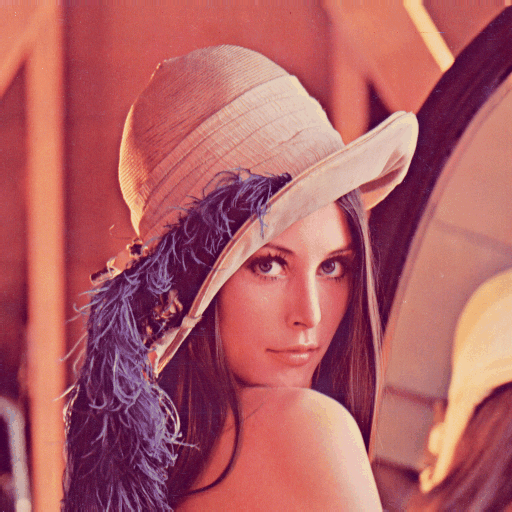
\includegraphics[width=0.3\textwidth]{./Images/lenna.png}
    \captionof{figure}{Lenna: Escena mixta con piel y texturas.}
\end{center}
\vspace{0.5cm}

\subsubsection*{Fresas}
Textura repetitiva de pequeño tamaño y color dominante saturado. Es útil para estudiar el manejo de microdetalles como son las semillas y la redundancia espacial sin perder estructura repetitiva.

En este caso esperamos que el compresor obtenga una buena tasa de compresión gracias a la repetición constante del patrón, pero también es probable que aparezca pérdida de detalle fino en las texturas pequeñas, y que las  tonalidades de las fresas tiendan a aumentar su parecido, especialmente después de la cuantificación. La saturación del color debería conservarse relativamente bien, pero los bloques uniformes podrían mostrar artefactos si el nivel de compresión es alto.
\begin{center}
    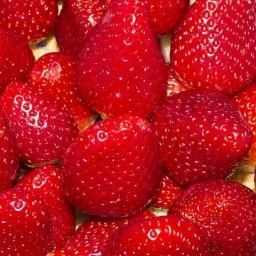
\includegraphics[width=0.3\textwidth]{./Images/fresas.png}
    \captionof{figure}{Fresas: Textura repetitiva y alta saturación.}
\end{center}
\vspace{0.5cm}

\subsubsection*{Cactus}
He seleccionado esta imagen porque combina un fondo plano con bordes de alto contraste entre luz y sombra, además de detalles finos como las espinas del cactus. Esto permite evaluar \textit{ringing} en los bordes, \textit{banding} en el cielo y pérdida de detalle en las espinas.

Queremos comprobar cómo maneja el compresor las transiciones abruptas entre el cielo y las espinas; asimismo, con una compresión alta, las plumas del pájaro podrían difuminarse y, si el compresor trata mal el cielo, podrían aparecer bandas.
\begin{center}
    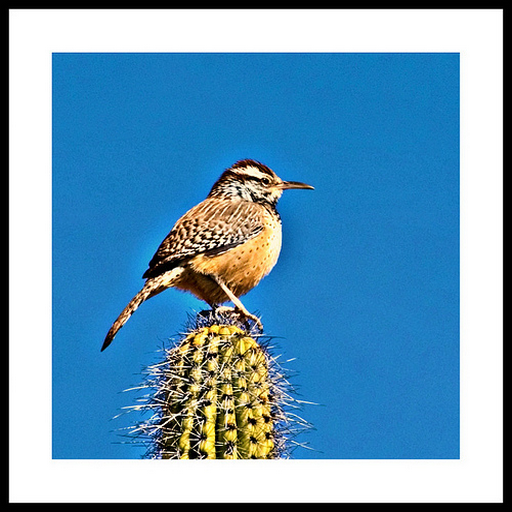
\includegraphics[width=0.3\textwidth]{./Images/cactus.png}
    \captionof{figure}{Cactus: Alto contraste y detalles finos.}
\end{center}
\vspace{0.5cm}

\subsubsection*{Grietas}
Líneas duras, diagonales y grietas irregulares hacen que esta imagen sea adecuada para evaluar fenómenos como el \textit{aliasing}, la deformación geométrica y la aparición de artefactos de bloque en zonas de alto contraste.

Se analiza si la compresión introduce artefactos de \textit{ringing} o
artefactos alrededor de las líneas oscuras de las grietas, consecuencia de la eliminación de altas frecuencias, así como si se preserva la nitidez del patrón de cuarteado sin que las líneas finas se vuelvan borrosas o se fusionen con el fondo.
\begin{center}
    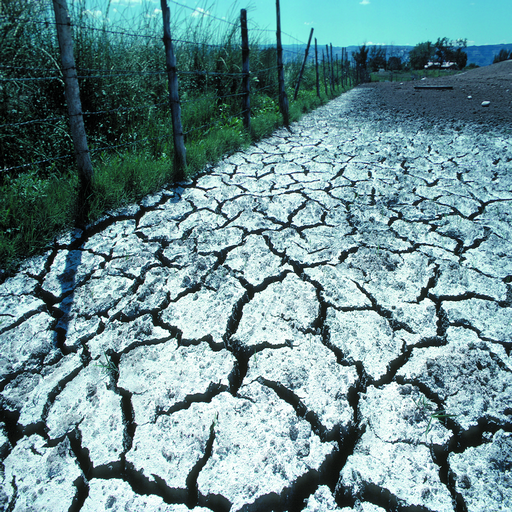
\includegraphics[width=0.3\textwidth]{./Images/grietas.png} 
    \captionof{figure}{Grietas: Líneas duras y diagonales.}
\end{center}
\vspace{0.5cm}

\subsubsection*{Brassica}
Esta imagen resulta muy interesante pues está llena de bordes irregulares bien definidos, una gran cantidad de detalles finos y transiciones severas de colores.

El objetivo es comprobar si al comprimir la imagen se suavizarán los bordes o se crearán artefactos de tipo anillo (ringing) perdiendo nitidez; evaluaremos cómo se distribuyen los errores en áreas complejas.
\begin{center}
    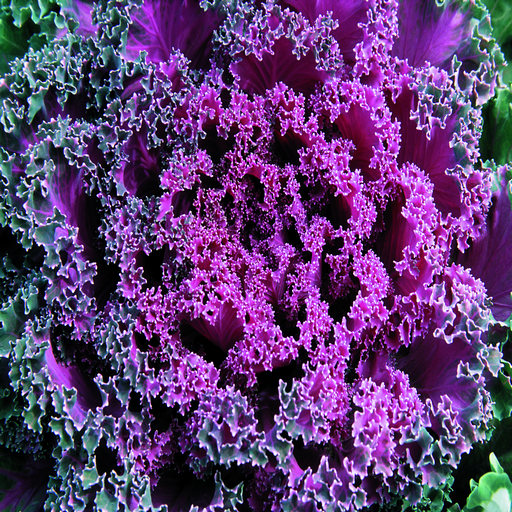
\includegraphics[width=0.3\textwidth]{./Images/brassica.png}
    \captionof{figure}{Brassica: Bordes irregulares y detalles finos.}
\end{center}
\vspace{0.5cm}

\subsubsection*{Colinas}
Esta imagen es interesante por su cielo claro, ya que presenta gradientes sutiles (transiciones de colores muy lentas). Queremos detectar si el compresor creará bandas o blocking en vez de continuar con las transiciones suaves.
\begin{center}
    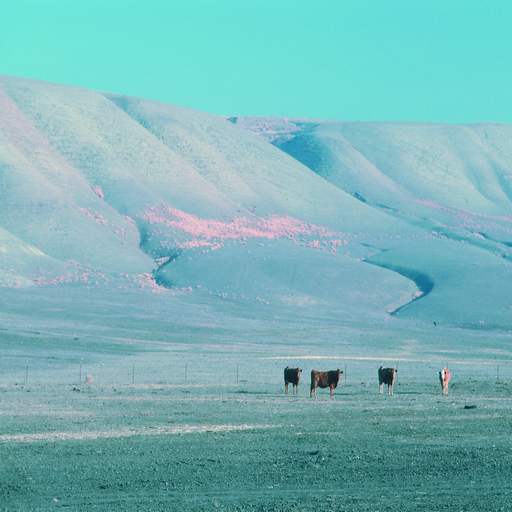
\includegraphics[width=0.3\textwidth]{./Images/colinas.png}
    \captionof{figure}{Colinas: Transiciones de luminancia suaves.}
\end{center}
\vspace{0.5cm}

\subsubsection*{Sailboat}
Hemos elegido esta imagen porque es la más completa: tiene zonas con muchísimo detalle (los pinos) y zonas muy limpias (cielo y agua). Además, el barco tiene líneas muy finas (el mástil).
El objetivo es analizar si esas líneas finas se mantienen nítidas o si aparecen "fantasmas" (artefactos). También servirá para ver si el compresor mantiene la textura de los pinos o los convierte en una mancha borrosa.
\begin{center}
    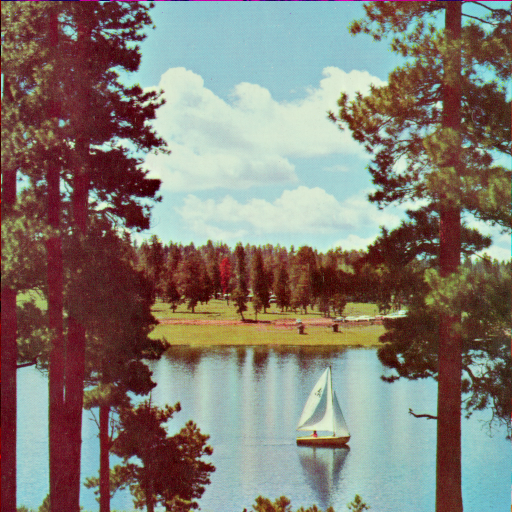
\includegraphics[width=0.3\textwidth]{./Images/sailboat.png}
    \captionof{figure}{Sailboat: Escena mixta con líneas finas y texturas.}
\end{center}
\vspace{0.5cm}

\subsubsection*{Uvas}
Seleccionada por la dificultad que presentan las formas esféricas juntas y la iluminación suave. No son colores planos, sino que tienen volumen y sombras.
El objetivo es ver cómo afecta la compresión a esa sensación de volumen (3D) y si respeta los matices de color o los apaga.
\begin{center}
    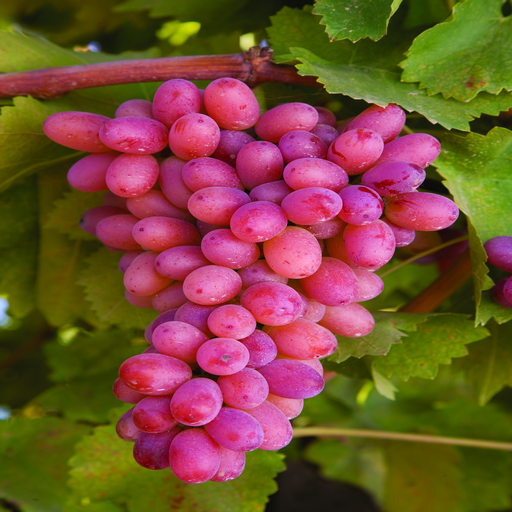
\includegraphics[width=0.3\textwidth]{./Images/uvas.png}
    \captionof{figure}{Uvas: Volumetría y degradados de color.}
\end{center}
\vspace{0.5cm}

\subsubsection*{Pino}

Representa un caso de "textura pura". Toda la imagen está llena de detalles rugosos, grietas profundas y alto contraste.
El objetivo es comprobar la resistencia del compresor ante altas frecuencias constantes.

\begin{center}
    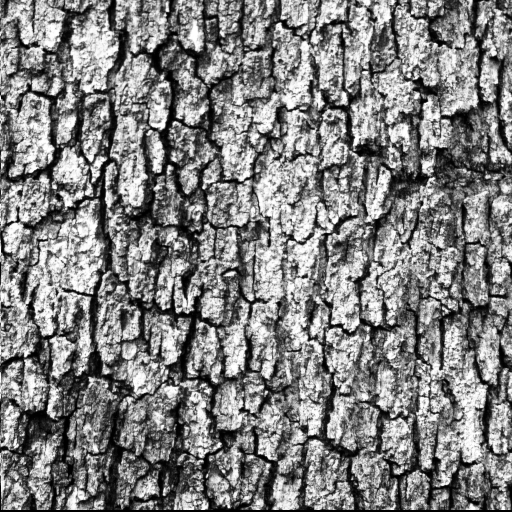
\includegraphics[width=0.3\textwidth]{./Images/pino.png}
    \captionof{figure}{Pino: Textura de alta frecuencia y alto contraste.}
\end{center}
\vspace{0.5cm}

\subsubsection{Estudio sobre la varianza}
Para el estudio experimental sobre el tiempo de ejecución, se realizó un filtrado previo sobre las imágenes seleccionadas anteriormente, calculando su varianza y entropía como métrica de complejidad. 

\begin{description}
    \item[Baja Complejidad (Varianza $<$ 2000):] Imágenes con predominio de zonas homogéneas (ej. \texttt{Fresas}).
    \item[Media Complejidad (2000 $<$ Varianza $<$ 4000):] Imágenes de uso común con equilibrio entre texturas y bordes (ej. \texttt{Lenna}).
    \item[Alta Complejidad (Varianza $>$ 4000):] Imágenes con alta densidad de detalles y texturas finas(ej. \texttt{Cactus}).
\end{description}


\subsubsection{Justificación de la métrica de clasificación}

Para clasificar la complejidad de las imágenes, se ha optado por realizar los cálculos sobre su versión en \textbf{escala de grises}. Esto se debe a que la información estructural de una imagen (bordes, formas y texturas) reside principalmente en su intensidad luminosa, y no en su color. Dado que el sistema visual humano es más sensible al brillo que al color, y que los algoritmos tipo JPEG priorizan la conservación de la luminancia, el análisis en escala de grises ofrece una estimación más realista de la información relevante.

Para cuantificar esta complejidad, se ha priorizado el uso de la \textbf{varianza} frente a la entropía. Mientras que la entropía mide la imprevisibilidad estadística (útil para la codificación), la varianza mide el contraste y la dispersión de los valores de los píxeles. Una varianza alta indica la presencia de cambios bruscos de intensidad y detalles finos (altas frecuencias). Dado que la transformada DCT tiene mayor dificultad para aproximar estas zonas de cambios rápidos sin introducir artefactos visuales, la varianza resulta ser el indicador más fiable.

 
% --- RESULTADOS --------------------------------------------------------------------


%-----------------------------------------------------------------------------------

\section{Resultados experimentales}
En esta sección analizamos los resultados obtenidos en los experimentos realizados. En primer lugar, abordamos el estudio cualitativo, cuyo objetivo es evaluar el grado de similitud percibido entre la imagen original y la comprimida, siguiendo los criterios definidos en la sección metodología.

A continuación, presentamos el análisis cuantitativo, basado en las métricas descritas en la sección 3.4.1 Para cada imagen y para ambos compresores, calculamos el Ratio de Compresión (RC), el Signal-to-Noise Ratio (SNR) y el Error Cuadrático Medio (MSE). Estas medidas proporcionan una valoración objetiva del rendimiento de los compresores y permiten establecer comparaciones claras entre ellos.

Por último, conviene remarcar que el análisis cualitativo sigue siendo esencial, ya que al final somos las personas quienes observamos las imágenes y juzgamos su calidad visual. No obstante, también es importante valorar los resultados desde una perspectiva teórica y cuantitativa, dado que el análisis cualitativo, aunque se intente aplicar con criterios uniformes, siempre está sujeto a un sesgo humano inherente. Ambos enfoques, por tanto, se complementan y ofrecen una visión más completa del comportamiento de los compresores.
\subsection{Sobre el análisis cualitativo}
Para el análisis visual de los resultados se han seleccionado cinco de los niveles de calidad generados por el compresor, considerando que presentar cinco calidades junto con la imagen original resulta más dinámico e informativo que mostrar únicamente tres. Los valores seleccionados han sido CaliQ 100, 200, 400, 800 y 1600, ya que permiten cubrir un rango amplio de degradación y facilitan una evaluación visual más completa del comportamiento del compresor.

Asimismo, se presenta un ejemplo de cómo se llevará a cabo la identificación sistemática de las calidades mediante comparaciones visuales entre la imagen original y sus versiones procesadas con distintos valores de \texttt{caliQ}. Este procedimiento permite determinar de manera objetiva el punto en el que la degradación se vuelve perceptible:

\begin{itemize}
    \item \textbf{caliQ = 100}
    \item \textbf{caliQ = 200}
    \item \textbf{caliQ = 400}
    \item \textbf{caliQ = 800}
    \item \textbf{caliQ = 1600}
\end{itemize}

Para cada nivel de \texttt{caliQ}, se comparará visualmente la versión comprimida con la original, evaluando la aparición de artefactos, pérdida de nitidez y suavizado de detalles finos. De esta manera, se establecerá un criterio sistemático para identificar las calidades a partir de la percepción de la degradación.


\textbf{Nota:} se puede apreciar que el formato anunciado puede no ser respetado en caso de encontrar situaciones de mayor interés analítico para el estudio.
\subsection{Sobre el análisis cuantitativo}

En este estudio se han establecido los siguientes rangos de referencia para la interpretación del MSE:
\begin{itemize}
    \item \textbf{MSE bajo--medio}: valores en torno a 500 o inferiores.
    \item \textbf{MSE medio}: valores comprendidos aproximadamente entre 700 y 850.
    \item \textbf{MSE alto}: valores superiores a dicho rango.
\end{itemize}

Estos umbrales se han definido tomando como referencia el mayor factor de calidad empleado (1600), ya que corresponde al escenario en el que el error introducido resulta más representativo.

A modo de presentación explicamos brevemente el formato en el que muestran los resultados:

\begin{center}
    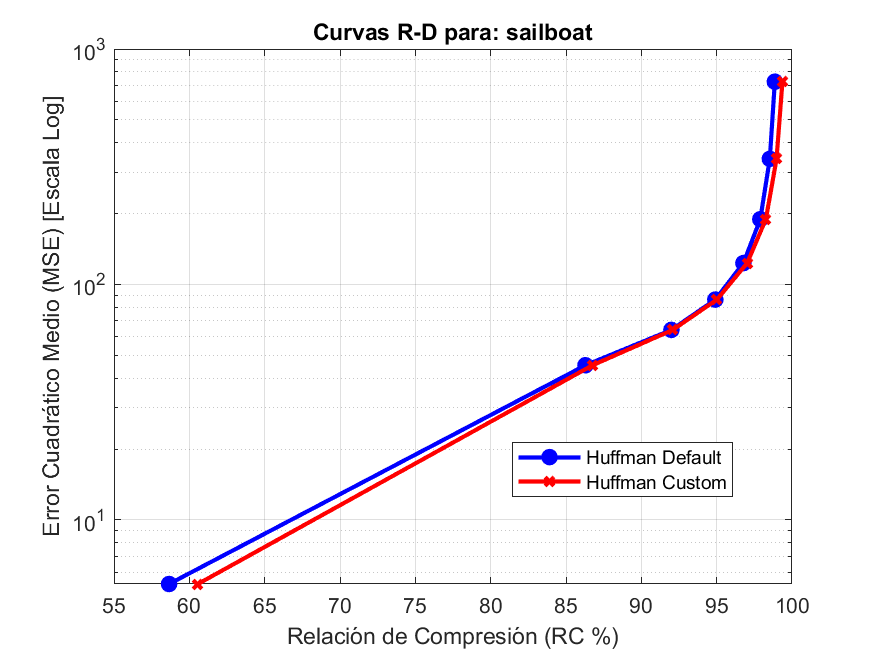
\includegraphics[width=0.8\textwidth]{../../source/Graficas/Grafica_sailboat.png}
    \captionof{figure}{Ejemplo: MSE vs RC (\%) en Escala Semilogarítmica.}
        \label{fig:mse_rc}
\end{center}
\vspace{0.5cm}

\begin{table}[h]
\centering
\csvautotabular{../../source/Results/sailboat.csv}
\caption{Ejemplo Tabla}
\label{tab:sailboat}
\end{table}
\vspace{0.5cm}


La Figura~\ref{fig:mse_rc} Presenta las curvas R--D en formato semilogarítmico. El eje X representa la Relación de Compresión (RC\,\%), donde valores altos implican mayor reducción del tamaño final. El eje Y muestra el Error Cuadrático Medio (MSE) en escala logarítmica, de forma que valores reducidos indican una reconstrucción más fiel.

Se comparan dos configuraciones:
\begin{itemize}
    \item \textbf{Huffman Default (Azul):} Tablas estándar del formato JPEG.
    \item \textbf{Huffman Custom (Rojo):} Tablas adaptadas a la estadística específica de la imagen de franjas.
\end{itemize}

Esta representación evidencia cómo el uso de tablas personalizadas desplaza la curva hacia la derecha, reflejando una mejor eficiencia de compresión para un mismo nivel de error.

La Tabla recoge los valores asociados a cada punto de las curvas. Los parámetros más relevantes son:

\begin{itemize}
    \item \textbf{CaliQ:} Factor de cuantificación utilizado en la compresión; valores mayores implican una mayor pérdida de información.
    \item \textbf{Dflt RC:} Relación de Compresión obtenida con tablas estándar.
    \item \textbf{Cst RC:} Relación de Compresión obtenida con tablas personalizadas.
\end{itemize}

Las métricas adicionales (MSE, PSNR) complementan la caracterización de la distorsión, aunque el énfasis en esta sección se centra en cómo evoluciona la Relación de Compresión y el error en función del parámetro \texttt{CaliQ}.
\subsection{Análisis cualitativo y cuantitativo}

%------------------------------------------------
\subsubsection*{Franjas} 

\begin{center} 
    
\includegraphics[width=0.3\textwidth]{./Images/franjas.png} 
    \hfill 
    
\includegraphics[width=0.3\textwidth]{../../source/Custom/franjas_Q100_Custom.png} 
    \hfill 
    
\includegraphics[width=0.3\textwidth]{../../source/Custom/franjas_Q200_Custom.png} 
     
    \captionof{figure}{Franjas: Comparativa visual con calidades: original, 100 y 200 (caliQ).} 
\end{center} 
\vspace{0.5cm} 

\begin{center} 
    
\includegraphics[width=0.3\textwidth]{../../source/Custom/franjas_Q400_Custom.png} 
    \hfill 
    
\includegraphics[width=0.3\textwidth]{../../source/Custom/franjas_Q800_Custom.png} 
    \hfill 
    
\includegraphics[width=0.3\textwidth]{../../source/Custom/franjas_Q1600_Custom.png} 
    \captionof{figure}{Franjas: Comparativa visual con calidades: 400, 800 y 1600 (caliQ).} 
\end{center} 
\vspace{0.5cm}

\subsubsection*{Análisis Cualitativo de Franjas}

El excelente rendimiento visual de esta imagen, incluso con valores de cuantificación extremos, se explica principalmente por la naturaleza matemática de la Transformada de Coseno Discreta (DCT) aplicada a zonas de color uniforme. Al dividir la imagen de 512×512 píxeles entre las 9 franjas, obtenemos un ancho aproximado de 56,88 píxeles por franja. Dado que la compresión opera en bloques de 8×8, estos bloques caen completamente dentro de un color sólido. En un bloque de color plano, la DCT es increíblemente eficiente: toda la información se concentra en un único punto (el coeficiente DC o frecuencia cero), mientras que el resto de coeficientes (AC) son cero. Como la compresión funciona eliminando o simplificando esos otros coeficientes, en este caso no hay nada que eliminar, por lo que el bloque se reconstruye perfecto o casi perfecto.

Respecto a la geometría las primeras 8 franjas se redondean a 56 píxeles, se acumula un sobrante de pixeles que otorga a la última franja un ancho de 64 píxeles exactos. Al ser 64 un múltiplo de 8, esta última franja encaja perfecta en el tamaño de bloque de la DCT, evitando bloques que contengan fronteras entre dos colores (donde suelen aparecer los errores). Sin embargo, la razón por la que los dos últimos colores (gris oscuro y negro) se fusionan en la Figura anterior no es por la alineación de los píxeles, sino por la severidad de la tabla de cuantificación.

La fusión de las últimas franjas ocurre porque el parámetro caliQ 1600 impone un paso de cuantificación tan grande que se empiezan a perder matices de color.

\subsubsection*{Análisis Cuantitativo de Franjas}

Desde el momento en que se seleccionó esta imagen, se esperaba un rendimiento excelente en términos de tamaño, debido al reducido número de colores presentes. Ambos compresores obtienen una tasa de compresión muy elevada desde las primeras calidades. En cuanto al error, el MSE se mantiene extremadamente bajo, incluso al alcanzar la degradación máxima dentro de nuestro rango de valores, observándose un aumento significativo únicamente en la compresión con CaliQ 1600.

Respecto a la tasa de compresión, los resultados son muy buenos desde el inicio. En el compresor \textit{default} se observa un incremento aproximado del 0,30\% al aplicar la máxima calidad. Resulta especialmente interesante comprobar que, aplicando únicamente el factor de calidad más bajo (CaliQ $5$) en el compresor \textit{custom}, ya se obtiene un resultado sobresaliente, incluso superior al mejor resultado alcanzado por el compresor \textit{default}.

En cuanto al SNR, los valores obtenidos son muy buenos y consistentes con el comportamiento del MSE. Solo se observa una degradación significativa en las calidades CaliQ 800 y 1600, confirmando que, en el resto de los casos, los píxeles originales se distinguen claramente del ruido introducido por el proceso de cuantificación, lo que refleja la excelente calidad de las reconstrucciones.


\begin{center}
    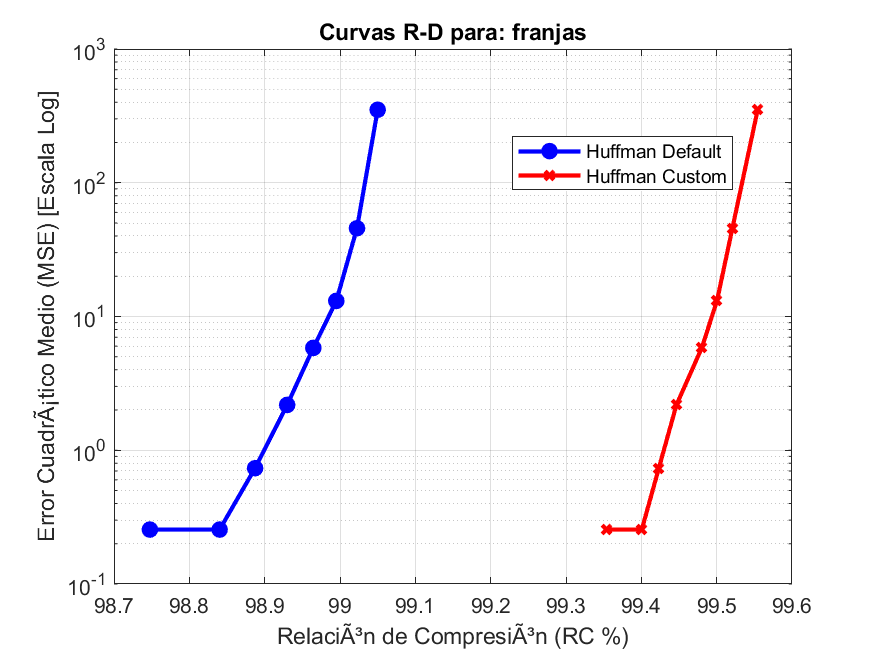
\includegraphics[width=0.8\textwidth]{../../source/Graficas/Grafica_franjas.png}
    \captionof{figure}{Franjas: MSE vs RC (\%) en Escala Semilogarítmica.}
\end{center}
\vspace{0.5cm}

\begin{table}[h]
\centering
\csvautotabular{../../source/Results/franjas.csv}
\caption{Resultados franjas}
\label{tab:franjas}
\end{table}
\vspace{0.5cm}

\subsubsection*{Conclusión franjas}
Finalmente, respecto a la hipótesis planteada acerca de que el resultado de la compresión sería excelente, esta se ha cumplido. No obstante, la expectativa de observar transiciones abruptas entre franjas no se ha visto satisfecha. Esto se debe, como se explicó anteriormente, a que la anchura de las franjas es múltiplo del tamaño de bloque, lo que evita la aparición de discontinuidades visibles.


% ---------------------------------------------------------

\subsubsection*{Lenna}

\begin{center} 
    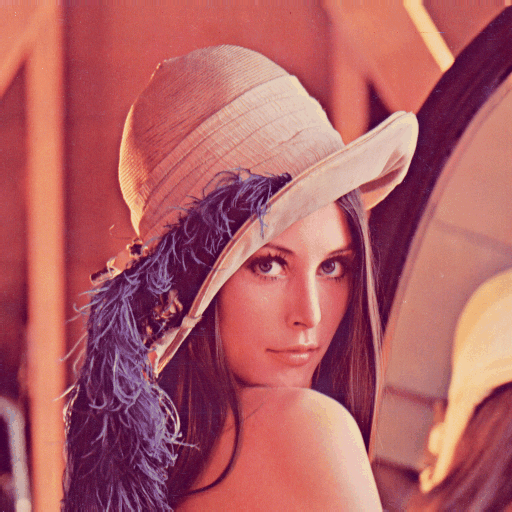
\includegraphics[width=0.3\textwidth]{./Images/lenna.png} 
    \hfill 
    \includegraphics[width=0.3\textwidth]{../../source/Custom/Lenna_Q100_Custom.png} 
    \hfill 
    \includegraphics[width=0.3\textwidth]{../../source/Custom/Lenna_Q200_Custom.png} 
     
    \captionof{figure}{Lenna: Comparativa visual con calidades: original, 100 y 200 (caliQ).} 
\end{center} 
\vspace{0.5cm} 

\begin{center} 
    \includegraphics[width=0.3\textwidth]{../../source/Custom/Lenna_Q400_Custom.png} 
    \hfill 
    \includegraphics[width=0.3\textwidth]{../../source/Custom/Lenna_Q800_Custom.png} 
    \hfill 
    \includegraphics[width=0.3\textwidth]{../../source/Custom/Lenna_Q1600_Custom.png} 
    \captionof{figure}{Lenna: Comparativa visual con calidades: 400, 800 y 1600 (caliQ).} 
\end{center} 
\vspace{0.5cm}

\subsubsection*{Análisis Cualitativo de Lenna}
La tasa de compresión obtenida en los primeros resultados no es muy alta, ya que la cuantificación aplicada no reduce significativamente el tamaño de la imagen. Sin embargo, al aplicar un factor de calidad ligeramente mayor, se logra una tasa de compresión mucho más satisfactoria, manteniendo una calidad prácticamente indistinguible de la imagen original y reduciendo su tamaño a aproximadamente una décima del original. Hasta la calidad $200$ se observa una mejora de compresión ligera pero significativa, del orden del $7\%$. Ambos compresores muestran un comportamiento muy similar en las tasas obtenidas, y los valores de SNR son consistentes con esta observación, reflejando que la calidad de las reconstrucciones se mantiene alta.

\begin{itemize}
    \item \textbf{caliQ = 100}: La imagen mantiene su nitidez; no se perciben diferencias relevantes respecto a la original.
    \item \textbf{caliQ = 200}: La calidad sigue siendo prácticamente idéntica. No se observan artefactos visibles.
    \item \textbf{caliQ = 400}: Primer nivel donde aparece degradación ligera; los detalles finos comienzan a suavizarse.
    \item \textbf{caliQ = 800}: La pérdida de calidad es clara, con aparición blocking y transiciones de color menos suaves.
    \item \textbf{caliQ = 1600}: Degradación severa; la imagen pierde detalle y presenta un aspecto muy borroso y cuadriculado.
\end{itemize}


\subsubsection*{Análisis Cuantitativo de Lenna}

\begin{center}
    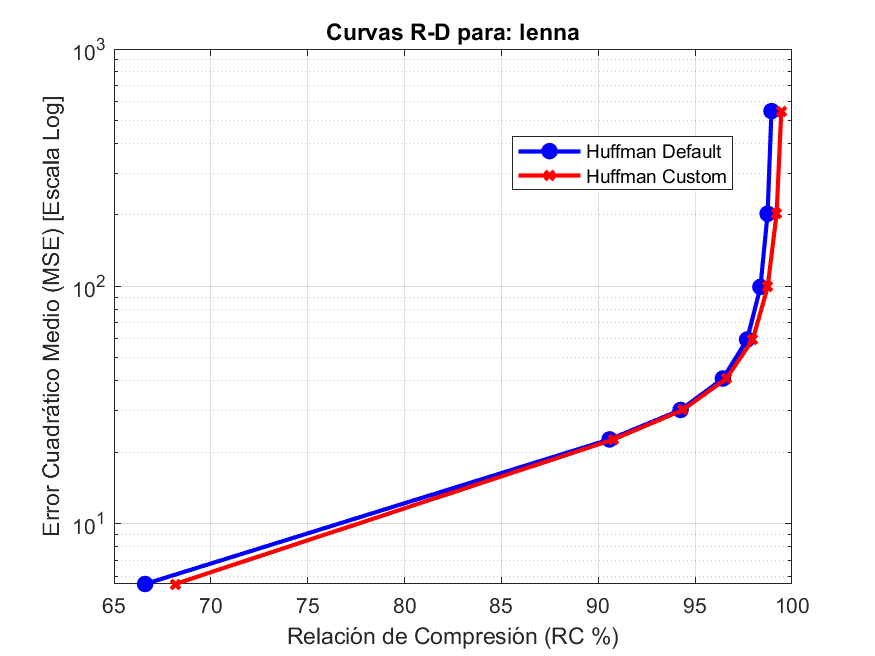
\includegraphics[width=1\textwidth]{../../source/Graficas/Grafica_lenna.png}
    \captionof{figure}{Lenna: MSE vs RC (\%) en Escala Semilogarítmica.}
\end{center}
\vspace{0.5cm}

\begin{table}[h]
\centering
\csvautotabular{../../source/Results/lenna.csv}
\caption{Resultados Lenna}
\label{tab:lenna}
\end{table}
\vspace{0.5cm}


\subsubsection*{Conclusión Lenna}
El objetivo de esta imagen era comprobar el comportamiento del compresor en una escena cotidiana con gran variedad de tonalidades. Se concluye que la modesta ganancia de compresión ($0.5\%$) obtenida al incrementar el factor \texttt{CaliQ} de $200$ a $400$ no justifica la notable degradación visual percibida en la imagen.

Respecto a los objetivos de evaluar la aparición de distintos artefactos, en calidades $100$ y $200$ no se observan diferencias significativas. A partir de la calidad $400$, se detectan algunos artefactos en el pelo del sombrero y en las transiciones suaves de color del fondo, así como la aparición de bloques por toda la imagen.

% ---------------------------------------------------------

\subsubsection*{Fresas}

\begin{center} 
    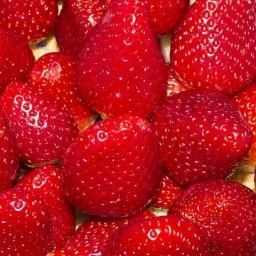
\includegraphics[width=0.3\textwidth]{./Images/fresas.png} 
    \hfill 
    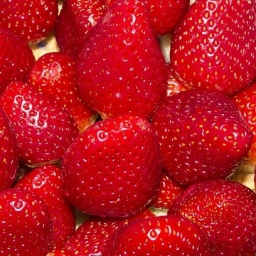
\includegraphics[width=0.3\textwidth]{../../source/Custom/fresas_Q100_Custom.png} 
    \hfill 
    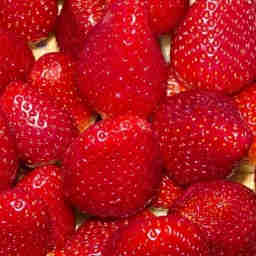
\includegraphics[width=0.3\textwidth]{../../source/Custom/fresas_Q200_Custom.png} 
     
    \captionof{figure}{Fresas: Comparativa visual con calidades: original, 100 y 200 (caliQ).} 
\end{center} 
\vspace{0.5cm} 

\begin{center} 
    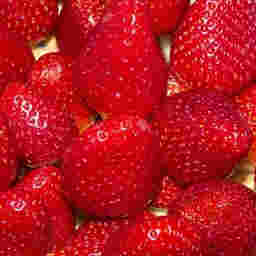
\includegraphics[width=0.3\textwidth]{../../source/Custom/fresas_Q400_Custom.png} 
    \hfill 
    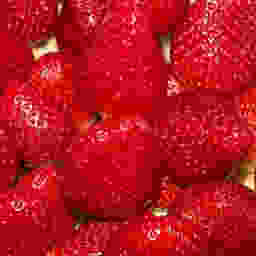
\includegraphics[width=0.3\textwidth]{../../source/Custom/fresas_Q800_Custom.png} 
    \hfill 
    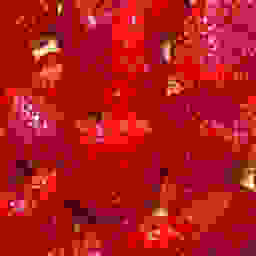
\includegraphics[width=0.3\textwidth]{../../source/Custom/fresas_Q1600_Custom.png} 
    \captionof{figure}{Fresas: Comparativa visual con calidades: 400, 800 y 1600 (caliQ).} 
\end{center} 
\vspace{0.5cm}

\subsubsection*{Análisis Cualitativo de Fresas}


\begin{itemize}
    \item \textbf{caliQ = 100}: La imagen mantiene su nitidez; no se perciben diferencias relevantes respecto a la original.
    \item \textbf{caliQ = 200}: La calidad empeora visualmente siendo perceptible pero conservando un grado aceptable algunas semillas se han suavizado.
    \item \textbf{caliQ = 400}: Aparece degradación alta los detalles, empieza a haber mucho blocking.
    \item \textbf{caliQ = 800}: La pérdida de calidad es clara, con blocking extendido por toda la imagen y transiciones de color menos suaves.
    \item \textbf{caliQ = 1600}: Degradación severa; la imagen se ha reducido a unas formas indistinguibles nada similares a la imagen original.
\end{itemize}

\subsubsection*{Análisis Cuantitativo de Fresas}

La imagen corresponde a un caso de error medio según nuestras métricas. No se trata de un escenario crítico ni de gran dificultad, pero tampoco se puede considerar un ejemplo de compresión perfecta.

El MSE aumenta progresivamente con el factor \texttt{CaliQ}, mientras que la RC alcanza valores altos a partir de calidades intermedias, reflejando una compresión eficiente sin degradar excesivamente la imagen. Los valores de PSNR son consistentes con esta interpretación, mostrando que la calidad se mantiene aceptable, aunque no óptima. En general, este caso permite evaluar el comportamiento del compresor en condiciones de dificultad moderada, ofreciendo referencias intermedias para comparar con casos más extremos.

\begin{center}
    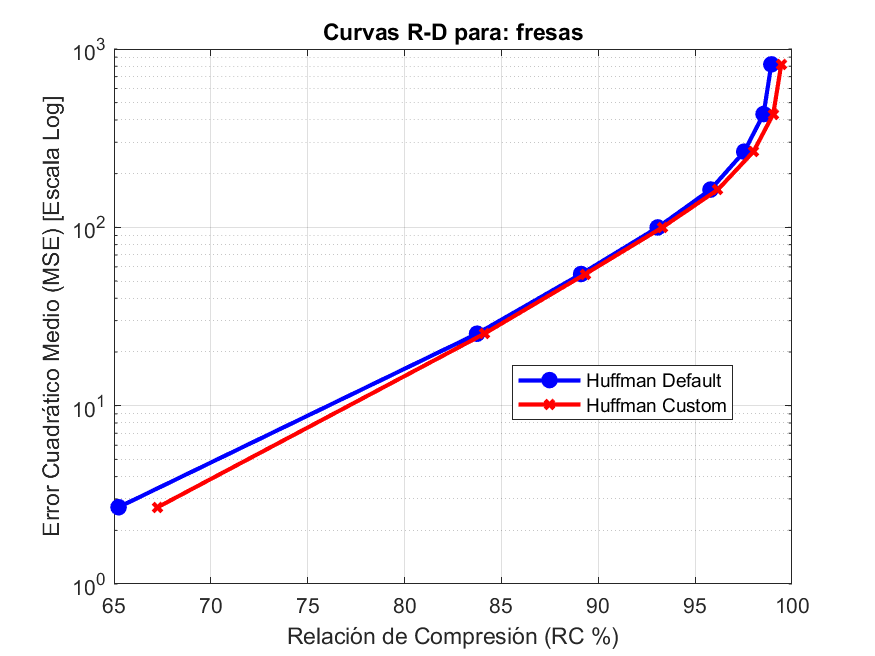
\includegraphics[width=1\textwidth]{../../source/Graficas/Grafica_fresas.png}
    \captionof{figure}{Fresas: MSE vs RC (\%) en Escala Semilogarítmica.}
\end{center}
\vspace{0.5cm}

\begin{table}[h]
\centering
\csvautotabular{../../source/Results/fresas.csv}
\caption{Resultados fresas}
\label{tab:fresas}
\end{table}
\vspace{0.5cm}


\subsubsection*{Conclusión Fresas}
El objetivo original consistía en evaluar cómo un patrón de textura repetitiva de pequeño tamaño y color dominante saturado afectaría la compresión y 
la preservación de microdetalles. Efectivamente, nuestro planteamiento se confirmó: la tasa de compresión obtenida ha sido buena y hemos observado una 
situación que podría compararse o utilizarse como analogía a un caso de imagen ya borrosa, dado que la imagen inicial presentaba cierta pérdida de 
nitidez debido a la uniformidad de la tonalidad. 

También observamos un efecto más pronunciado en comparación con otros resultados, ya que las dimensiones de esta imagen eran $256 \times 256$, lo que incrementa la sensación de pérdida de calidad. Este detalle debe tenerse en cuenta al interpretar los resultados.

% ---------------------------------------------------------

\subsubsection*{Cactus}

\begin{center} 
    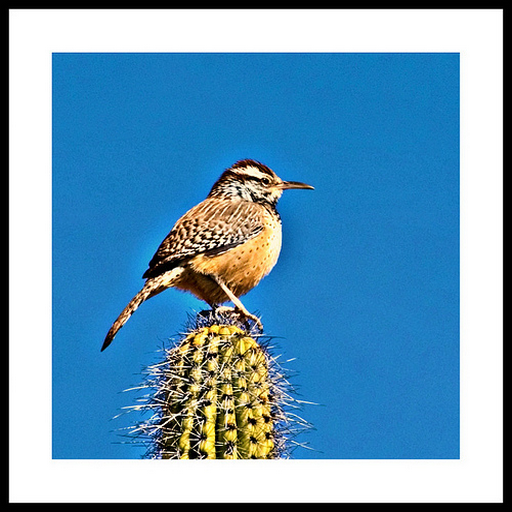
\includegraphics[width=0.3\textwidth]{./Images/cactus.png} 
    \hfill 
    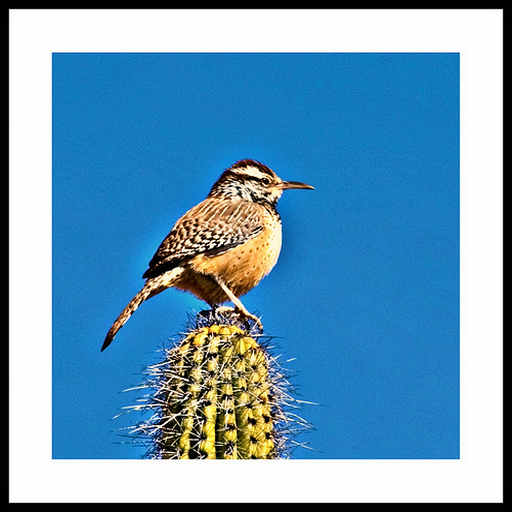
\includegraphics[width=0.3\textwidth]{../../source/Custom/cactus_Q100_Custom.png} 
    \hfill 
    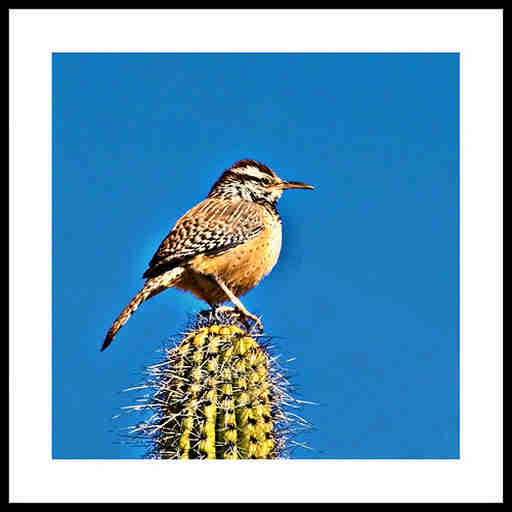
\includegraphics[width=0.3\textwidth]{../../source/Custom/cactus_Q200_Custom.png} 
     
    \captionof{figure}{Cactus: Comparativa visual con calidades: original, 100 y 200 (caliQ).} 
\end{center} 
\vspace{0.5cm} 

\begin{center} 
    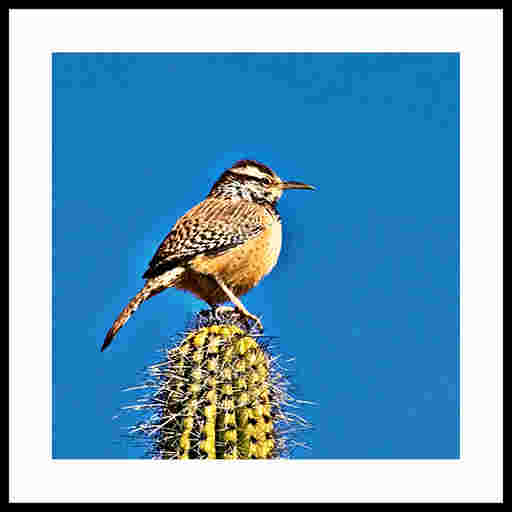
\includegraphics[width=0.3\textwidth]{../../source/Custom/cactus_Q400_Custom.png} 
    \hfill 
    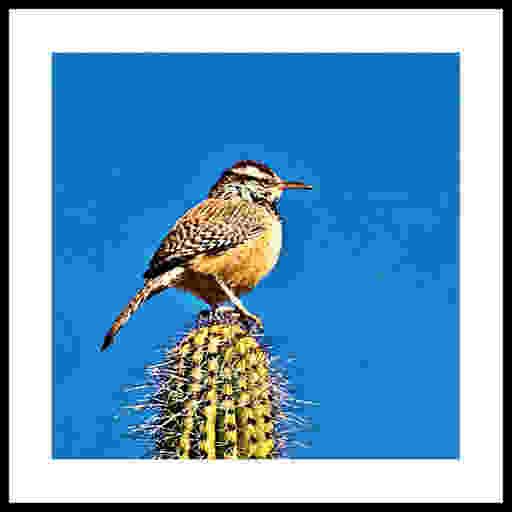
\includegraphics[width=0.3\textwidth]{../../source/Custom/cactus_Q800_Custom.png} 
    \hfill 
    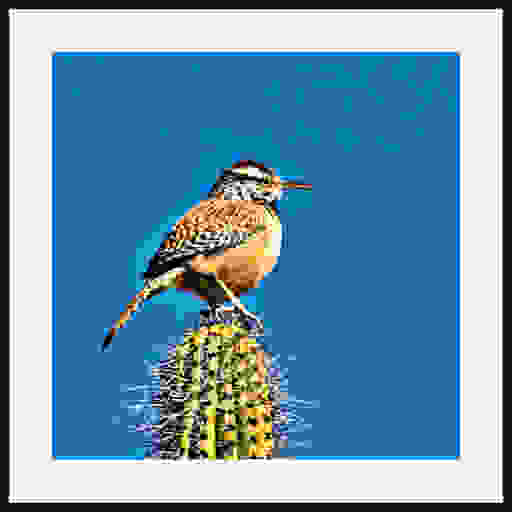
\includegraphics[width=0.3\textwidth]{../../source/Custom/cactus_Q1600_Custom.png} 
    \captionof{figure}{Cactus: Comparativa visual con calidades: 400, 800 y 1600 (caliQ).} 
\end{center} 
\vspace{0.5cm}

\subsubsection*{Análisis Cualitativo de Cactus}


\begin{itemize}
    \item \textbf{caliQ = 100}: La imagen mantiene su nitidez; no se perciben diferencias relevantes respecto a la original.
    \item \textbf{caliQ = 200}: La calidad se ve afectada sutilmente por la aparición de banding en el cielo y en el contorno del pájaro.
    \item \textbf{caliQ = 400}: El banding se hace mucho más evidente, empeorando los degradados y deteriorando la impresión general. Tanto el pájaro como el cactus conservan una nitidez aceptable, aunque las espinas pierden algo de detalle y definición.
    \item \textbf{caliQ = 800}: La figura del pájaro se conserva bien, pero su contorno empeora notablemente. Los tonos del cielo se reducen a dos tonalidades y las espinas del cactus se deterioran significativamente.
    \item \textbf{caliQ = 1600}: Degradación severa; aparecen colores nuevos, se pierde completamente el detalle en las espinas del cactus y el pájaro se ve extremadamente pixelado, borroso y cuadriculado.
\end{itemize}


\subsubsection*{Análisis cuantitativo}

Las transiciones suaves (degradados) se representan con bajas y medias frecuencias, no con altas (que representan el detalle fino/ruido). El banding es la manifestación de que las bajas/medias frecuencias que describen la variación gradual del color se han redondeado demasiado, creando "escalones" en el tono

respecto a la tasa de compresión obtenida es bastante promedio y no hay una diferencia significativa real entre el compresor custom y el default pues la diferencia no supera el 0.5\% en factores de calidad realistas como 100 y 200.
La tasa de compresión es buena pues haz zonas muy uniformes de colores como el marco  y el cielo. 

El SNR no tiene una medida muy buena es otra forma mas de confirmar que esta imagen es mas difícil para el compresor que otras.

\begin{center}
    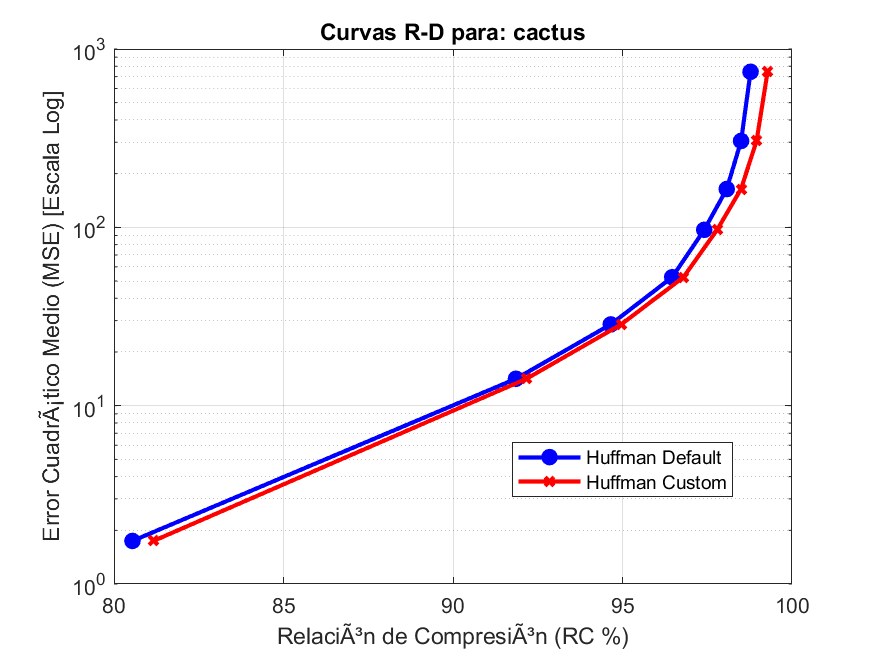
\includegraphics[width=1\textwidth]{../../source/Graficas/Grafica_cactus.png}
    \captionof{figure}{Cactus: MSE vs RC (\%) en Escala Semilogarítmica.}
\end{center}
\vspace{0.5cm}

\begin{table}[h]
\centering
\csvautotabular{../../source/Results/cactus.csv}
\caption{Resultados Cactus}
\label{tab:cactus}
\end{table}
\vspace{0.5cm}


\subsubsection*{Conclusión Cactus}
Esta imagen fue elegida por su cielo degradado y la cantidad de detalles que tenía, tanto en el pájaro como en las espinas del cactus. En el análisis cualitativo, hemos comprobado, como esperábamos, que las transiciones de color del cielo se perdían por la aparición de banding. También esperábamos la pérdida de detalle en el plumaje del cactus wren; sin embargo, esto no ha sido así. Respecto a las espinas, visualmente no se ha detectado ringing; quizás un análisis más detallado revelaría este artefacto.

Para esta imagen, la calidad elegida sería $100$, un buen equilibrio entre compresión y nitidez. La calidad $200$ sería una buena opción si se fuese a mostrar en un tamaño pequeño.

% ---------------------------------------------------------

\subsubsection*{Grietas}

\begin{center} 
    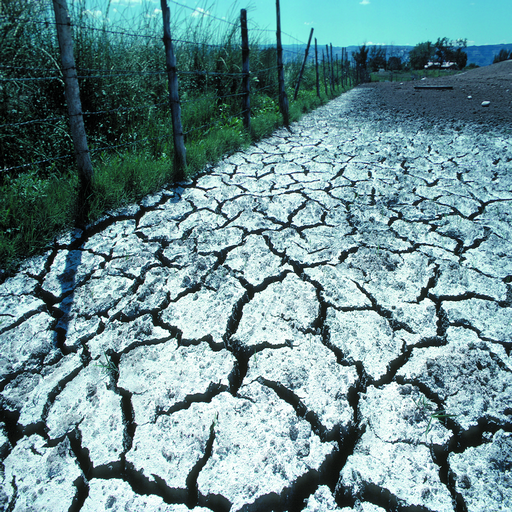
\includegraphics[width=0.3\textwidth]{./Images/grietas.png} 
    \hfill 
    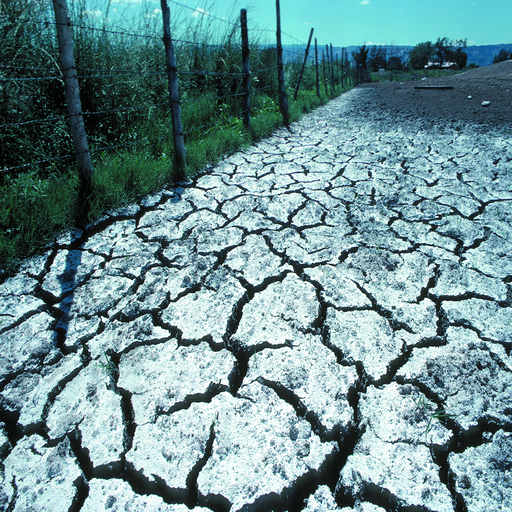
\includegraphics[width=0.3\textwidth]{../../source/Custom/grietas_Q100_Custom.png} 
    \hfill 
    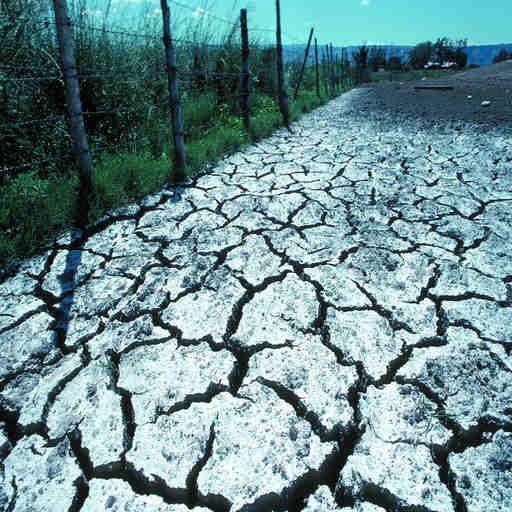
\includegraphics[width=0.3\textwidth]{../../source/Custom/grietas_Q200_Custom.png} 
     
    \captionof{figure}{Grietas: Comparativa visual con calidades: original, 100 y 200 (caliQ).} 
\end{center} 
\vspace{0.5cm} 

\begin{center} 
    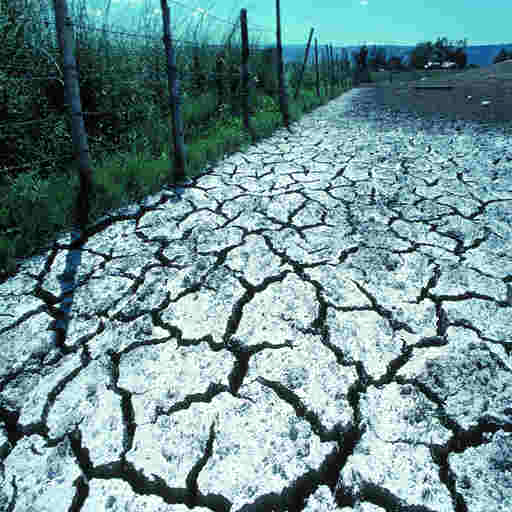
\includegraphics[width=0.3\textwidth]{../../source/Custom/grietas_Q400_Custom.png} 
    \hfill 
    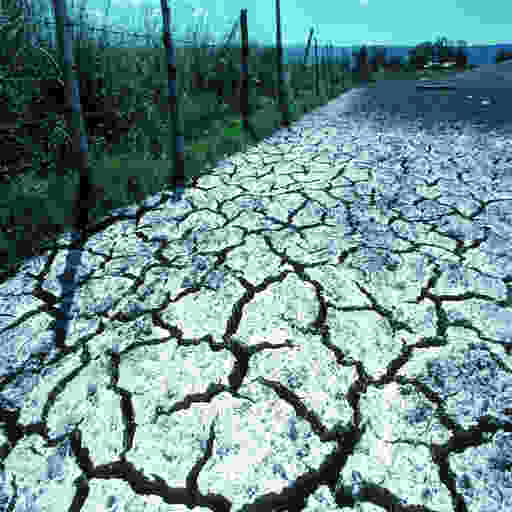
\includegraphics[width=0.3\textwidth]{../../source/Custom/grietas_Q800_Custom.png} 
    \hfill 
    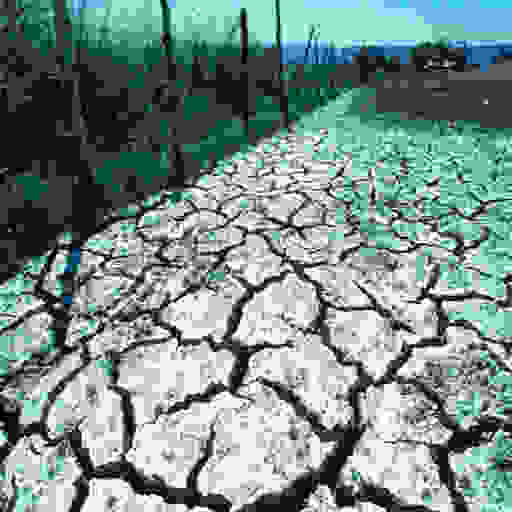
\includegraphics[width=0.3\textwidth]{../../source/Custom/grietas_Q1600_Custom.png} 
    \captionof{figure}{Grietas: Comparativa visual con calidades: 400, 800 y 1600 (caliQ).} 
\end{center} 
\vspace{0.5cm}


\subsubsection*{Análisis Cualitativo de Grietas}


\begin{itemize}
    \item \textbf{caliQ = 100}: La imagen mantiene su nitidez; no se perciben diferencias relevantes respecto a la original.
    \item \textbf{caliQ = 200}: La imagen pierde ligeramente nitidez, pero conserva correctamente los detalles.
    \item \textbf{caliQ = 400}: Aparece banding en el cielo y el fondo comienza a verse borroso, aunque el frente se mantiene bien; se introduce un leve ringing en las grietas.
    \item \textbf{caliQ = 800}: La imagen se ve afectada significativamente por la cuantificación; las tonalidades del suelo cambian y las plantas y el fondo se convierten en bloques de color, perdiendo casi todo detalle, aunque las grietas se conservan.
    \item \textbf{caliQ = 1600}: Degradación severa. Los colores de las grietas mejoran visualmente de manera fortuita, pero los colores del fondo y las plantas se pierden completamente. Las grietas se conservan bien, probablemente porque su color negro puede representarse con el primer componente AC de cada bloque, sin necesidad de coeficientes de alta frecuencia.
\end{itemize}

\subsubsection*{Análisis Cuantitativo de Grietas}

La imagen de la grieta ha resultado ser una de las más desafiantes para el compresor. Incluso con caliQ muy bajo, se obtuvo una tasa de compresión deficiente en ambos compresores y un SNR bajo. Las tasas de compresión obtenidas para esta imagen, tanto con calidades estándar como con calidades deseables, son bajas en comparación con las de las demás imágenes analizadas hasta el momento.


\begin{center}
    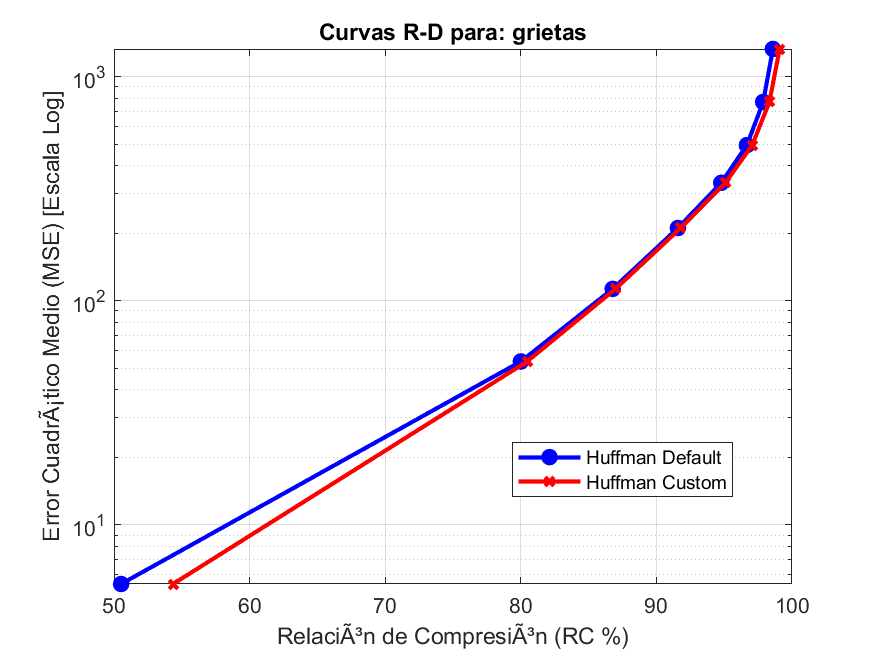
\includegraphics[width=1\textwidth]{../../source/Graficas/Grafica_grietas.png}
    \captionof{figure}{Grietas: MSE vs RC (\%) en Escala Semilogarítmica.}
\end{center}
\vspace{0.5cm}

\begin{table}[h]
\centering
\csvautotabular{../../source/Results/grietas.csv}
\caption{Resultados Grietas}
\label{tab:grietas}
\end{table}
\vspace{0.5cm}

\subsubsection*{Conclusión Grietas}
La conclusión obtenida es muy interesante: aunque no se observó el aliasing que se esperaba, encontramos un caso muy difícil para el compresor. Lo más sorprendente es cómo se conservan las grietas de la imagen, mientras que el suelo queda prácticamente en blanco y negro y el fondo se vuelve indistinguible. El frente de la imagen se aprecia correctamente a pesar de haberse utilizado una cuantificación tan severa.  

Esto destaca un resultado muy sorprendente: un caso tan difícil para el compresor produce dos comportamientos visuales distintos dentro de la misma imagen: una parte relativamente fácil de comprimir y otra muy difícil.

% ---------------------------------------------------------

\subsubsection*{Brassica}

\begin{center} 
    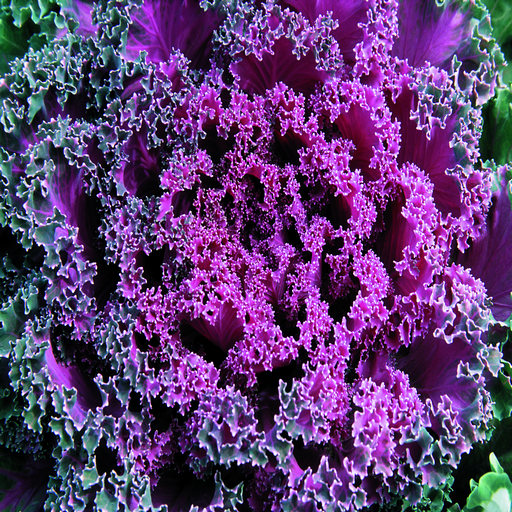
\includegraphics[width=0.3\textwidth]{./Images/brassica.png} 
    \hfill 
    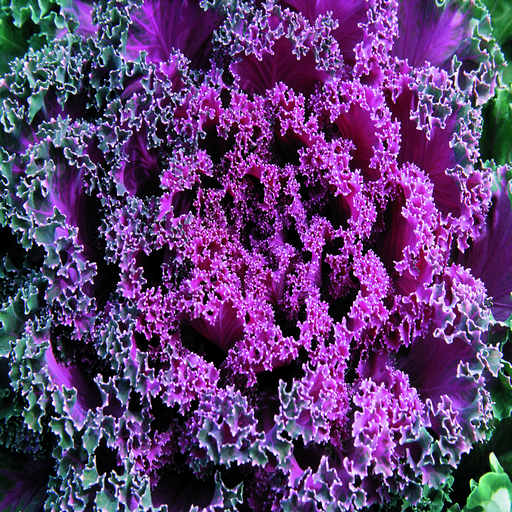
\includegraphics[width=0.3\textwidth]{../../source/Custom/brassica_Q100_Custom.png} 
    \hfill 
    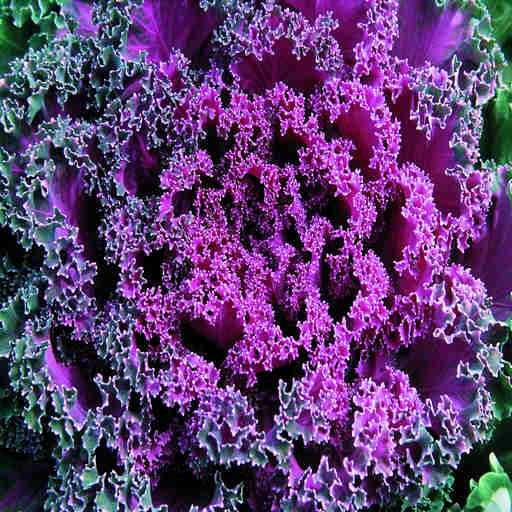
\includegraphics[width=0.3\textwidth]{../../source/Custom/brassica_Q200_Custom.png} 
     
    \captionof{figure}{Brassica: Comparativa visual con calidades: original, 100 y 200 (caliQ).} 
\end{center} 
\vspace{0.5cm} 

\begin{center} 
    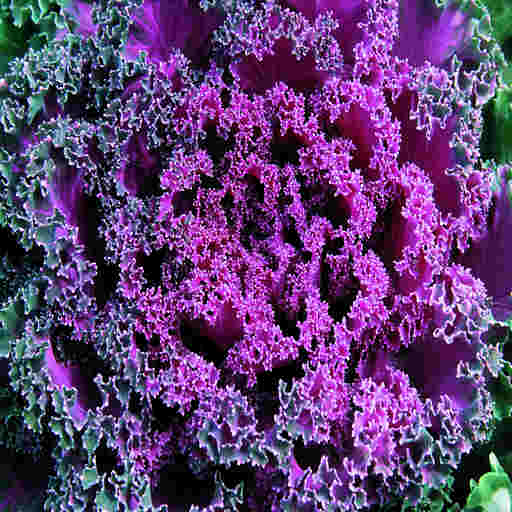
\includegraphics[width=0.3\textwidth]{../../source/Custom/brassica_Q400_Custom.png} 
    \hfill 
    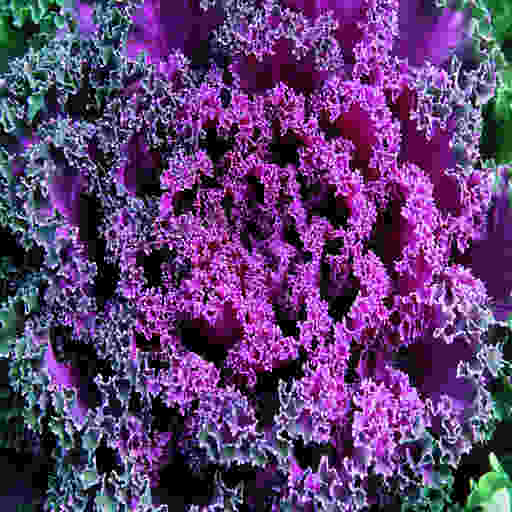
\includegraphics[width=0.3\textwidth]{../../source/Custom/brassica_Q800_Custom.png} 
    \hfill 
    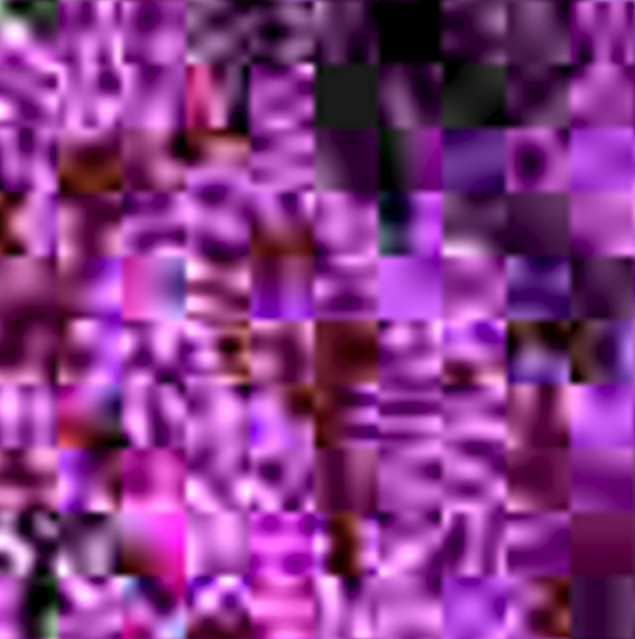
\includegraphics[width=0.3\textwidth]{./Images/zoom_brassica.jpg} 
    \captionof{figure}{Brassica: Comparativa visual con calidades: 400, 800 y 1600 (caliQ).} 
\end{center} 
\vspace{0.5cm}
 
\subsubsection*{Análisis Cualitativo de Brassica}

\begin{itemize}
    \item \textbf{caliQ = 100}: La imagen mantiene su nitidez; no se perciben diferencias relevantes respecto a la original.
    \item \textbf{caliQ = 200}: La imagen pierde ligeramente nitidez, pero conserva correctamente los detalles.
    \item \textbf{caliQ = 400}: La imagen comienza a verse borrosa en las zonas con detalles más pequeños, como el centro. También se observan algo de blocking y banding en las hojas exteriores, especialmente en la zona morada de la brassica. Los bordes han perdido forma y definición.
    \item \textbf{caliQ = 800}: Se aprecia blocking y banding en toda la imagen; los bordes de las hojas más centrales ya no son distinguibles y aparecen algunos bloques con ruido.
    \item \textbf{caliQ = 1600}: Ampliando el centro de la imagen hasta ver los bloques de $8 \times 8$ píxeles, se observa que la cuantización es tan fuerte que prácticamente ha eliminado toda la información de alta frecuencia. En cada bloque sólo quedan el coeficiente DC y algunos coeficientes de baja frecuencia. Al conservar tan pocos coeficientes, la imagen pierde continuidad y comienzan a hacerse visibles las propias funciones base de la DCT; en algunos bloques incluso se podría inferir cuáles coeficientes permanecen tras la cuantización.
\end{itemize}

\subsubsection*{Análisis Cuantitativo de Brassica}

El MSE obtenido para esta imagen es elevado desde el principio, lo que podemos asociar a una alta complejidad para el compresor.  

Respecto a la tasa de compresión, se observa que es baja incluso para factores de calidad bajos, lo que indica nuevamente que esta era una imagen complicada para el compresor. La diferencia entre ambos compresores a partir de caliQ $100$ es inferior al $0.5\%$, por lo que no resulta remarcable.  

El SNR también era bajo desde el inicio, obteniéndose resultados poco satisfactorios. 

\begin{center}
    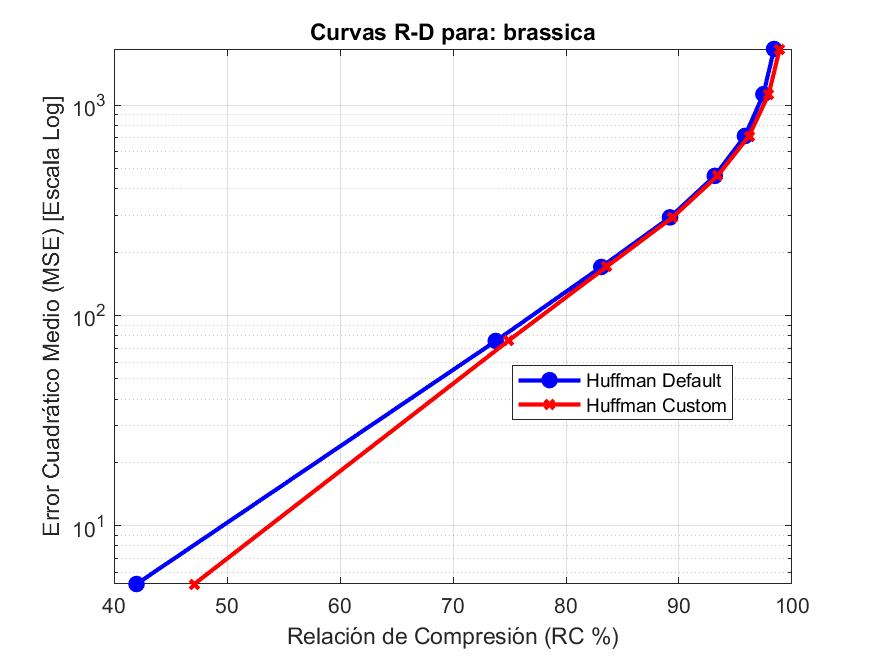
\includegraphics[width=1\textwidth]{../../source/Graficas/Grafica_brassica.png}
    \captionof{figure}{Brassica: MSE vs RC (\%) en Escala Semilogarítmica.}
\end{center}
\vspace{0.5cm}

\begin{table}[h]
\centering
\csvautotabular{../../source/Results/brassica.csv}
\caption{Resultados Brassica}
\label{tab:brassica}
\end{table}
\vspace{0.5cm}

 

\subsubsection*{Conclusión Brassica}
El objetivo de esta imagen era comprobar cómo se comportaba el compresor en situaciones con muchos bordes irregulares de pequeño tamaño. Hemos visto que estos bordes eran demasiado pequeños; el compresor funcionaba correctamente con factores de calidad inferiores a $200$, pero al ser los detalles tan finos se perdían, generándose bloques.  

Las tres métricas utilizadas nos llevan a la conclusión de que esta es una imagen con una dificultad de compresión superior a lo normal. Aunque aparentemente la imagen contaba con pocas tonalidades, finalmente esto no fue así.


% ---------------------------------------------------------

\subsubsection*{Colinas}

\begin{center} 
    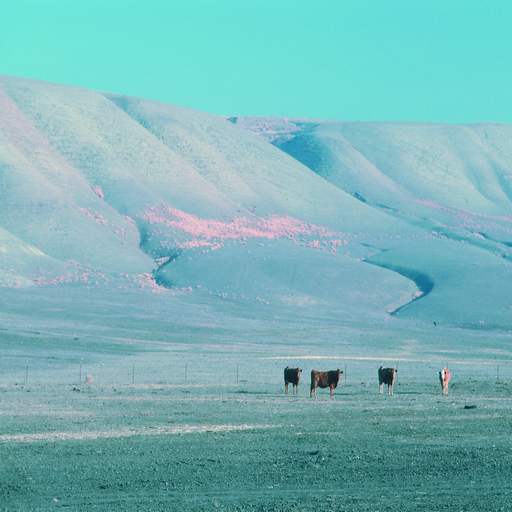
\includegraphics[width=0.3\textwidth]{./Images/colinas.png} 
    \hfill 
    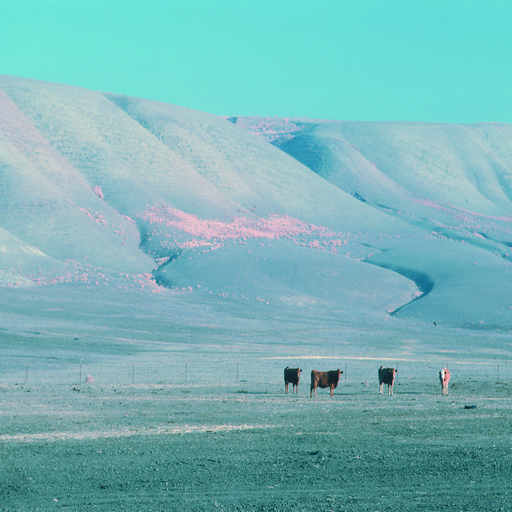
\includegraphics[width=0.3\textwidth]{../../source/Custom/colinas_Q100_Custom.png} 
    \hfill 
    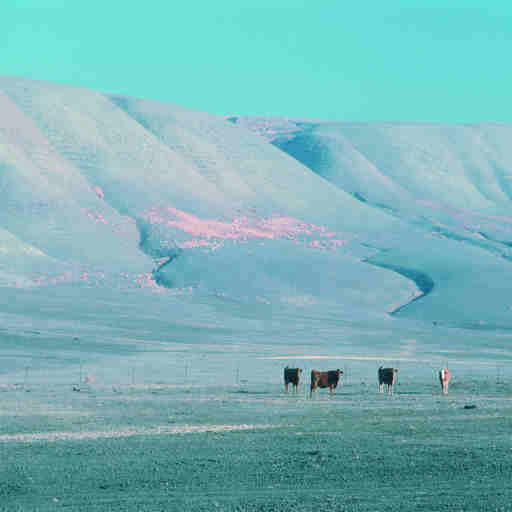
\includegraphics[width=0.3\textwidth]{../../source/Custom/colinas_Q200_Custom.png} 
     
    \captionof{figure}{Colinas: Comparativa visual con calidades: original, 100 y 200 (caliQ).} 
\end{center} 
\vspace{0.5cm} 

\begin{center} 
    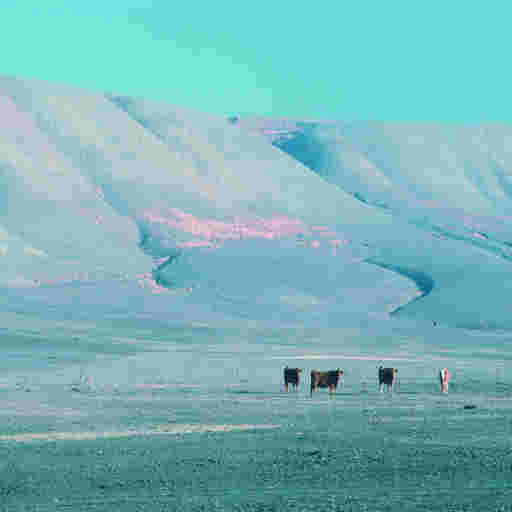
\includegraphics[width=0.3\textwidth]{../../source/Custom/colinas_Q400_Custom.png} 
    \hfill 
    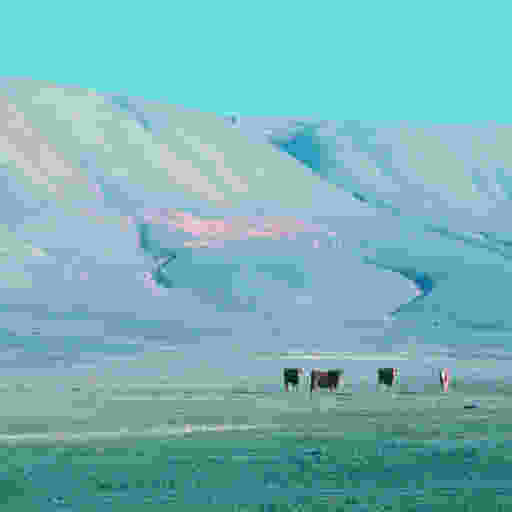
\includegraphics[width=0.3\textwidth]{../../source/Custom/colinas_Q800_Custom.png} 
    \hfill 
    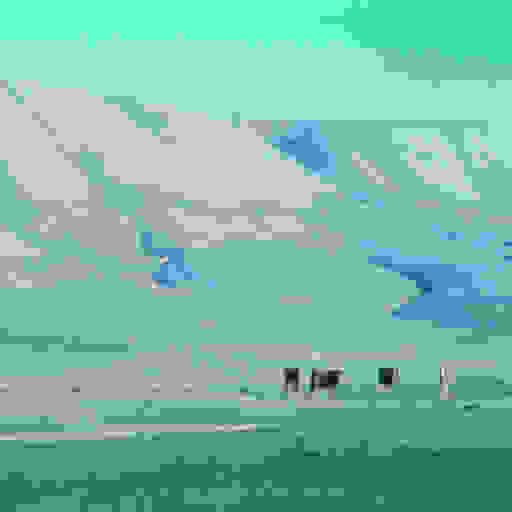
\includegraphics[width=0.3\textwidth]{../../source/Custom/colinas_Q1600_Custom.png} 
    \captionof{figure}{Colinas: Comparativa visual con calidades: 400, 800 y 1600 (caliQ).} 
\end{center} 
\vspace{0.5cm}

\subsubsection*{Análisis Cualitativo de Colinas}

\begin{itemize}
    \item \textbf{caliQ = 100}: La imagen mantiene su nitidez; no se perciben diferencias relevantes respecto a la original.
    \item \textbf{caliQ = 200}: Comienza a aparecer un ligero banding en el cielo, pero la imagen mantiene una nitidez excelente.
    \item \textbf{caliQ = 400}: El banding se incrementa en el cielo y aparece blocking en el resto de la imagen.
    \item \textbf{caliQ = 800}: Los artefactos se intensifican notablemente, especialmente el banding en el cielo, y comienza a apreciarse ringing en los bordes de las colinas.
    \item \textbf{caliQ = 1600}: El blocking es muy evidente; los bloques de $8 \times 8$ píxeles quedan prácticamente reducidos a un único color, lo que indica que todos los coeficientes de luminancia han sido anulados salvo el componente DC.
\end{itemize}

\subsubsection*{Análisis Cuantitativo de Colinas}

Se obtiene una tasa de compresión excelente desde factores de calidad muy bajos, concretamente a partir de $25$, con diferencias poco significativas al aumentar la calidad.

El MSE se sitúa en un rango bajo–medio y no se incrementa de forma suave a medida que aumentan los factores de calidad.

El SNR presenta valores adecuados, indicando un buen nivel de distorsión para los niveles de compresión aplicados.


\begin{center}
    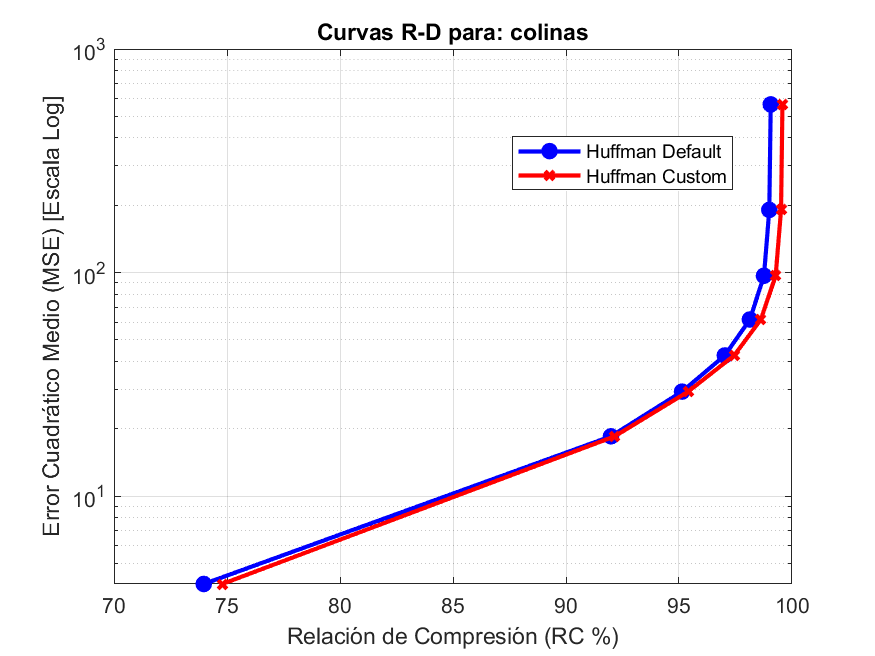
\includegraphics[width=1\textwidth]{../../source/Graficas/Grafica_colinas.png}
    \captionof{figure}{Colinas: MSE vs RC (\%) en Escala Semilogarítmica.}
\end{center}
\vspace{0.5cm}

\begin{table}[h]
\centering
\csvautotabular{../../source/Results/colinas.csv}
\caption{Resultados colinas}
\label{tab:colinas}
\end{table}
\vspace{0.5cm}


\subsubsection*{Conclusión para colinas}
Esta imagen era ideal para analizar el comportamiento del compresor ante gradientes suaves y cambios progresivos de tonalidad. El resultado obtenido ha sido el esperado: se alcanza un buen equilibrio entre compresión y distorsión.

La imagen ha resultado ser un caso favorable para el compresor, confirmándose nuestra hipótesis de que aparecería banding en el cielo y blocking en niveles de cuantificación elevados. En conjunto, el resultado ha sido satisfactorio.




% ---------------------------------------------------------
 
\subsubsection*{Sailboat}

\begin{center} 
    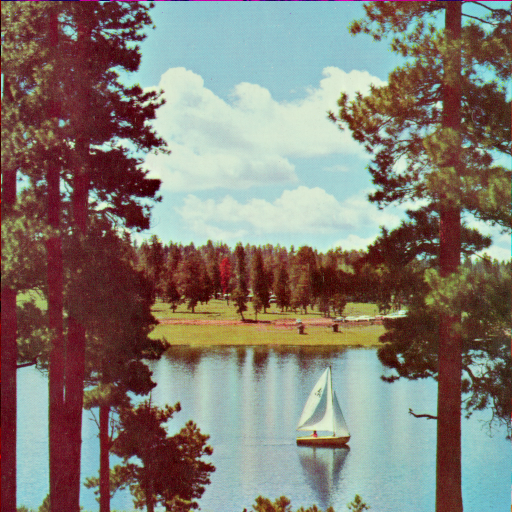
\includegraphics[width=0.3\textwidth]{./Images/sailboat.png} 
    \hfill 
    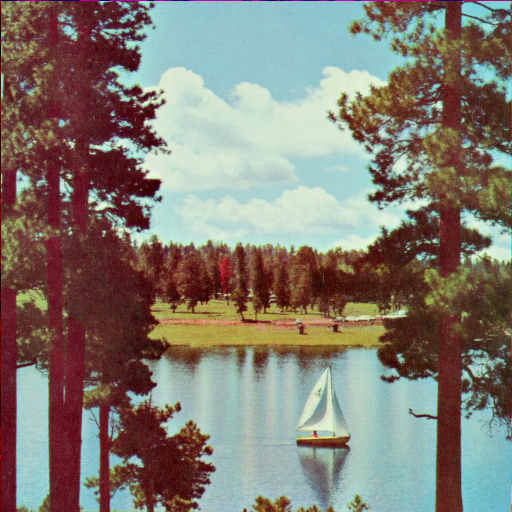
\includegraphics[width=0.3\textwidth]{../../source/Custom/sailboat_Q100_Custom.png} 
    \hfill 
    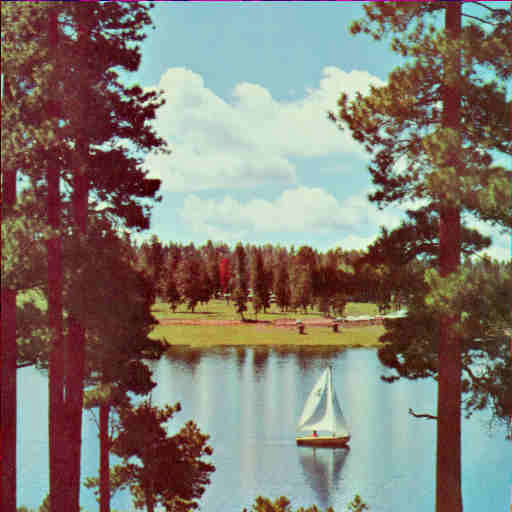
\includegraphics[width=0.3\textwidth]{../../source/Custom/sailboat_Q200_Custom.png} 
     
    \captionof{figure}{sailboat: Comparativa visual con calidades: original, 100 y 200 (caliQ).} 
\end{center} 
\vspace{0.5cm} 

\begin{center} 
    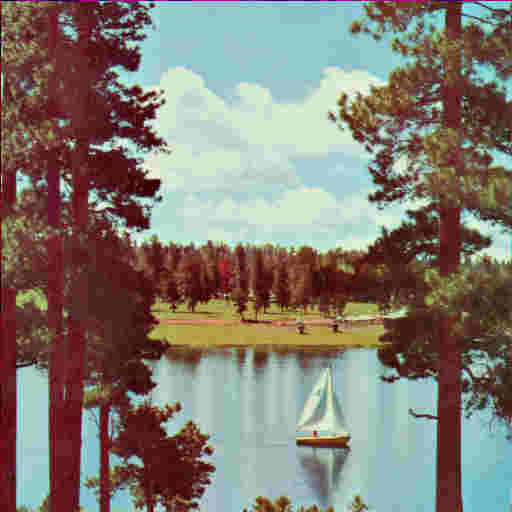
\includegraphics[width=0.3\textwidth]{../../source/Custom/sailboat_Q400_Custom.png} 
    \hfill 
    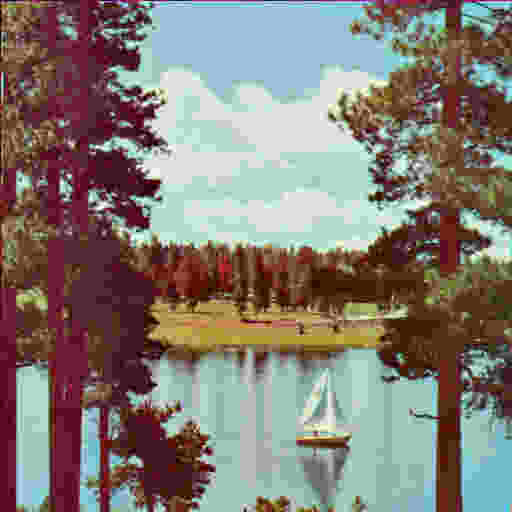
\includegraphics[width=0.3\textwidth]{../../source/Custom/sailboat_Q800_Custom.png} 
    \hfill 
    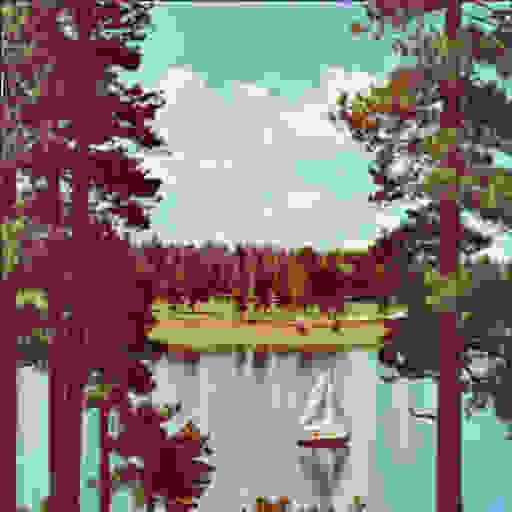
\includegraphics[width=0.3\textwidth]{../../source/Custom/sailboat_Q1600_Custom.png} 
    \captionof{figure}{sailboat: Comparativa visual con calidades: 400, 800 y 1600 (caliQ).} 
\end{center} 
\vspace{0.5cm}

\subsubsection*{Análisis Cualitativo de Sailboat}

\begin{itemize}
    \item \textbf{caliQ = 100}: La imagen mantiene su nitidez; no se perciben diferencias relevantes respecto a la original.
    \item \textbf{caliQ = 200}: La imagen se conserva bien, apareciendo algo de banding en las nubes, el cielo, el agua y los troncos de los árboles.
    \item \textbf{caliQ = 400}: El banding se agrava visualmente, pero la imagen todavía se ve correctamente, sin una pérdida de calidad significativa.
    \item \textbf{caliQ = 800}: El blocking y el banding se vuelven muy evidentes; las hojas de los árboles se transforman en masas sin forma y aparece blocking generalizado.
    \item \textbf{caliQ = 1600}: La degradación es severa: el fondo se vuelve indistinguible, el agua pierde su color, y los objetos presentan formas borrosas y mal definidas con mezclas de color severas, dando un resultado muy deficiente.
\end{itemize}


\subsubsection*{Análisis Cuantitativo de Sailboat}
El MSE obtenido para esta imagen es medio, obteniéndose una lectura deficiente para la primera calidad, pero mejorando considerablemente en las calidades posteriores. El SNR es coherente con los resultados, quizás ligeramente inferior a lo habitual, pero aceptable.  

Nuevamente, la diferencia entre el compresor \textit{custom} y el \textit{default} no ha sido significativa, sin superar el $0.5\%$ en los últimos resultados.


\begin{center}
    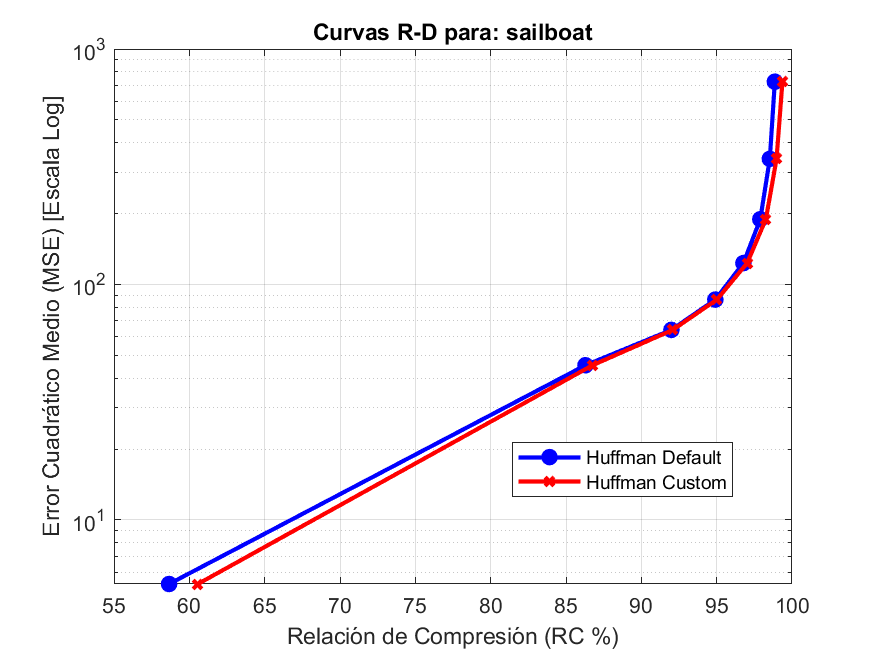
\includegraphics[width=1\textwidth]{../../source/Graficas/Grafica_sailboat.png}
    \captionof{figure}{sailboat: MSE vs RC (\%) en Escala Semilogarítmica.}
\end{center}
\vspace{0.5cm}

\begin{table}[h]
\centering
\csvautotabular{../../source/Results/sailboat.csv}
\caption{Resultados Sailboat}
\label{tab:sailboat}
\end{table}
\vspace{0.5cm}

\subsubsection*{Conclusión Sailboat}
En esta imagen encontramos características similares a la anterior, además de poder comprobar los objetivos planteados, como analizar si las líneas finas se mantienen nítidas. En este caso, los pinos se han convertido en manchas borrosas y las las lineas del barco se han perdido. 

Además, queríamos comparar el comportamiento del compresor con dos imágenes que compartían características similares, como Colinas, que era una imagen un poco más sencilla. En comparación, esta imagen resultó ser de dificultad media, obteniéndose un resultado aproximadamente lineal, con un error MSE aproximadamente el doble que en la imagen más sencilla.



% ---------------------------------------------------------

\subsubsection*{Uvas}

\begin{center} 
    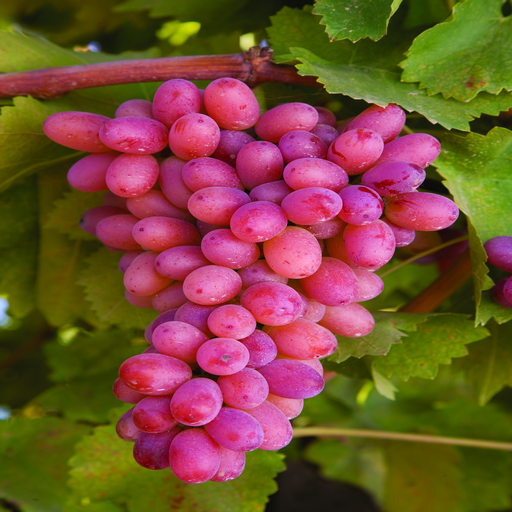
\includegraphics[width=0.3\textwidth]{./Images/uvas.png} 
    \hfill 
    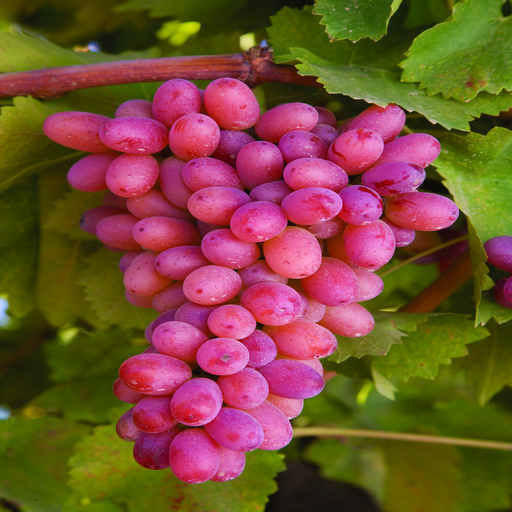
\includegraphics[width=0.3\textwidth]{../../source/Custom/uvas_Q100_Custom.png} 
    \hfill 
    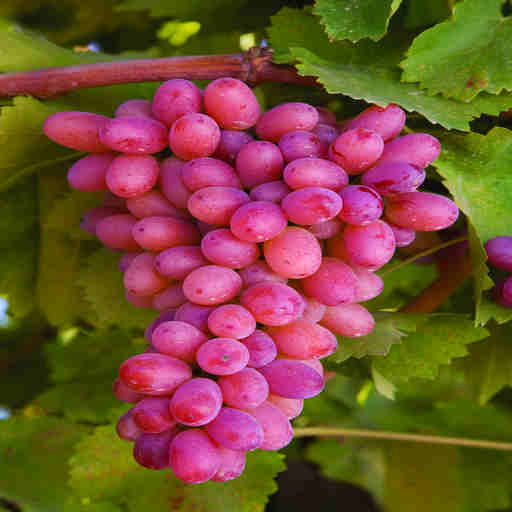
\includegraphics[width=0.3\textwidth]{../../source/Custom/uvas_Q200_Custom.png} 
    
    \captionof{figure}{Uvas: Comparativa visual con calidades: original, 100 y 200 (caliQ).} 
\end{center} 
\vspace{0.5cm} 

\begin{center} 
    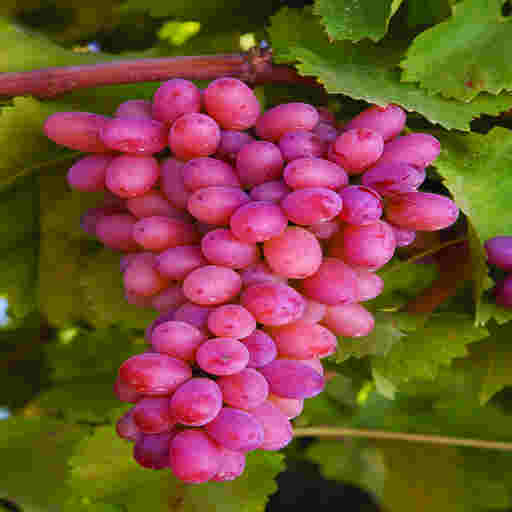
\includegraphics[width=0.3\textwidth]{../../source/Custom/uvas_Q400_Custom.png} 
    \hfill 
    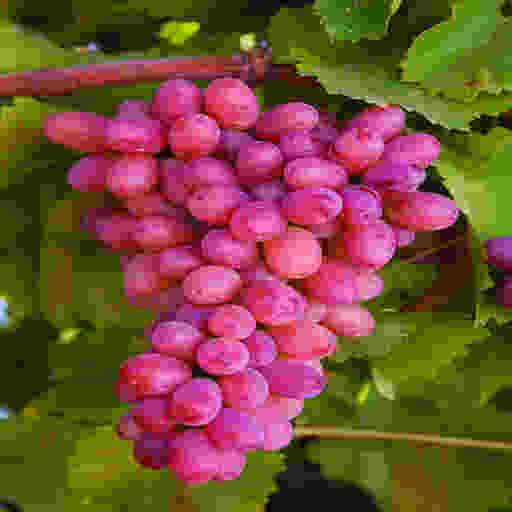
\includegraphics[width=0.3\textwidth]{../../source/Custom/uvas_Q800_Custom.png} 
    \hfill 
    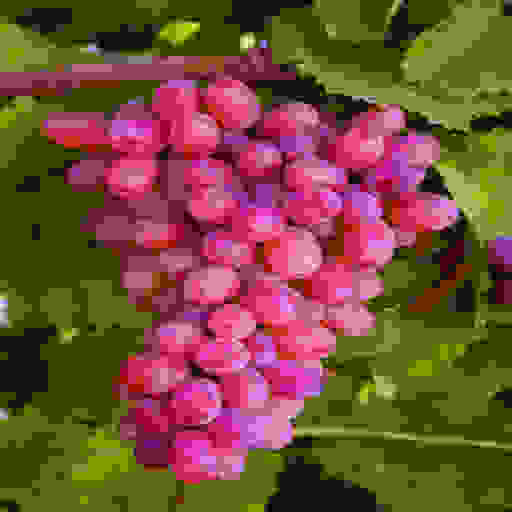
\includegraphics[width=0.3\textwidth]{../../source/Custom/uvas_Q1600_Custom.png} 
    \captionof{figure}{Uvas: Comparativa visual con calidades: 400, 800 y 1600 (caliQ).} 
\end{center} 
\vspace{0.5cm}

\subsubsection*{Análisis Cualitativo Uvas}
\begin{itemize}
    \item \textbf{caliQ = 100}: La imagen mantiene su nitidez; se introduce un ligero ringing en los bordes de las uvas.
    \item \textbf{caliQ = 200}: El ringing se agrava, pero la imagen no presenta defectos visuales graves.
    \item \textbf{caliQ = 400}: Aparece blocking de forma superficial en las uvas, generando una ligera sensación de borrosidad, y de forma más visible en las hojas del fondo.
    \item \textbf{caliQ = 800}: Todos los artefactos se incrementan de manera severa, afectando notablemente a la percepción global de la imagen.
    \item \textbf{caliQ = 1600}: Se pierden las formas esféricas de las uvas, dando lugar a una imagen plana y sin textura; las hojas presentan banding y las uvas se convierten en masas borrosas de color.
\end{itemize}

\subsubsection*{Análisis Cuantitativo Uvas}

\begin{center}
    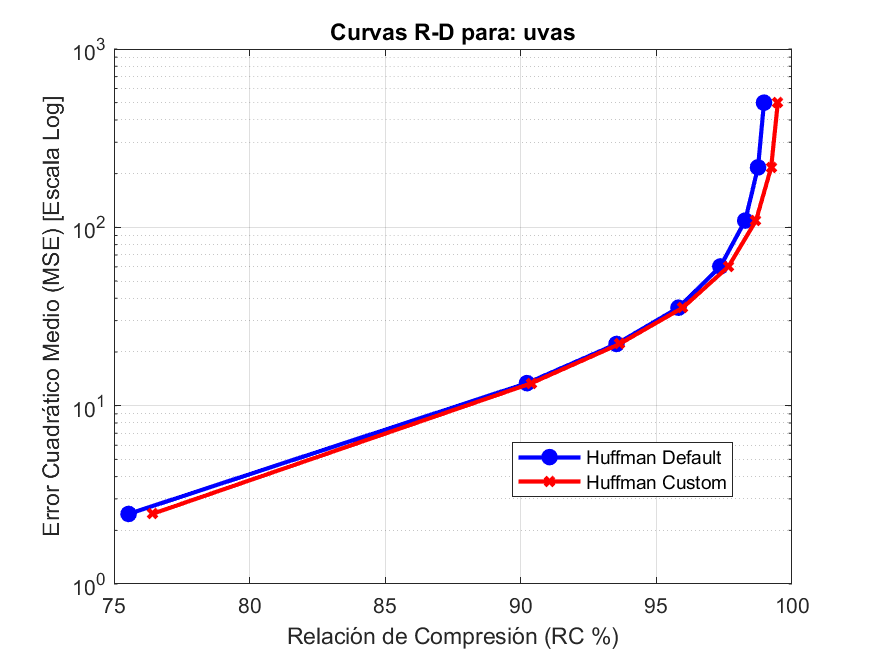
\includegraphics[width=1\textwidth]{../../source/Graficas/Grafica_uvas.png}
    \captionof{figure}{uvas: MSE vs RC (\%) en Escala Semilogarítmica.}
\end{center}
\vspace{0.5cm}

\begin{table}[h]
    \centering
    \csvautotabular{../../source/Results/uvas.csv}
    \caption{Resultados Uvas}
    \label{tab:uvas}
\end{table}
\vspace{0.5cm}

Se han obtenido niveles de distorsión buenos, similares a los observados en la imagen de colinas.

La tasa de compresión en este caso es excelente, lo que se debe al número reducido y a la uniformidad de los colores, tal y como era esperable.

La diferencia obtenida entre ambos compresores no es significativa.

Las medidas de ruido son buenas, en línea con los resultados observados anteriormente.


\subsubsection*{Conclusión Uvas}
Esta imagen fue seleccionada por sus formas esféricas, con el objetivo de analizar a partir de qué nivel de compresión los objetos comenzaban a aplanarse. Las conclusiones obtenidas han sido positivas, ya que no se ha percibido esta sensación hasta el factor de calidad más alto.

%-------------------------------------------------------------------------------

\subsubsection*{Pino}

\begin{center} 
    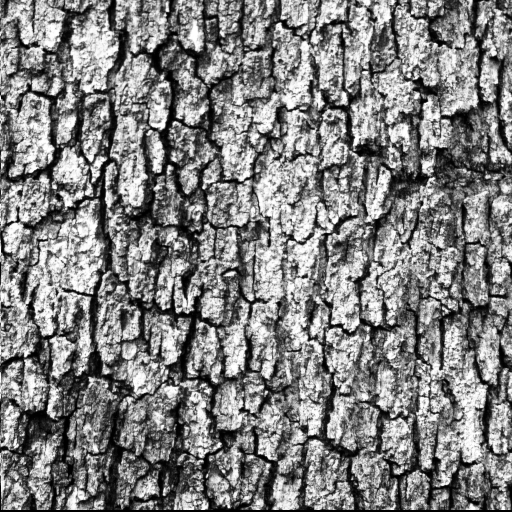
\includegraphics[width=0.3\textwidth]{./Images/pino.png} 
    \hfill 
    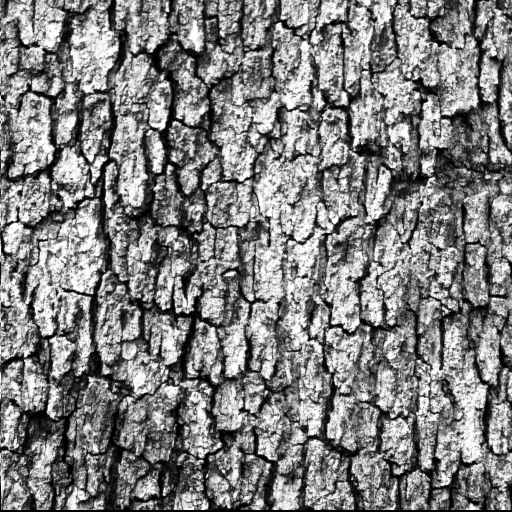
\includegraphics[width=0.3\textwidth]{../../source/Custom/pino_Q100_Custom.png} 
    \hfill 
    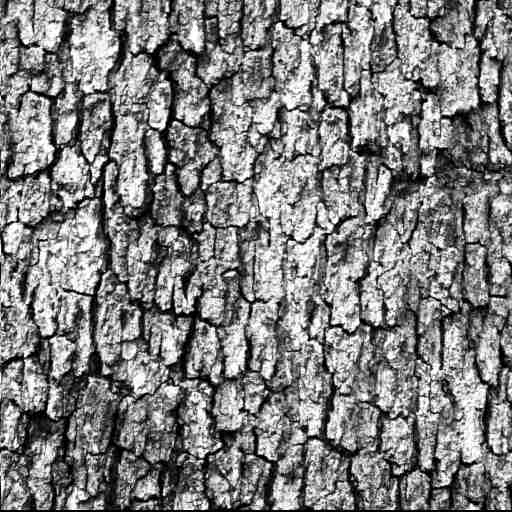
\includegraphics[width=0.3\textwidth]{../../source/Custom/pino_Q200_Custom.png} 
     
    \captionof{figure}{Pino: Comparativa visual con calidades: original, 100 y 200 (caliQ).} 
\end{center} 
\vspace{0.5cm} 

\begin{center} 
    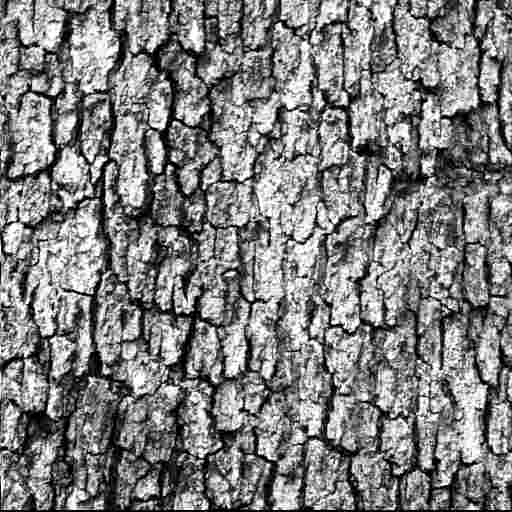
\includegraphics[width=0.3\textwidth]{../../source/Custom/pino_Q400_Custom.png} 
    \hfill 
    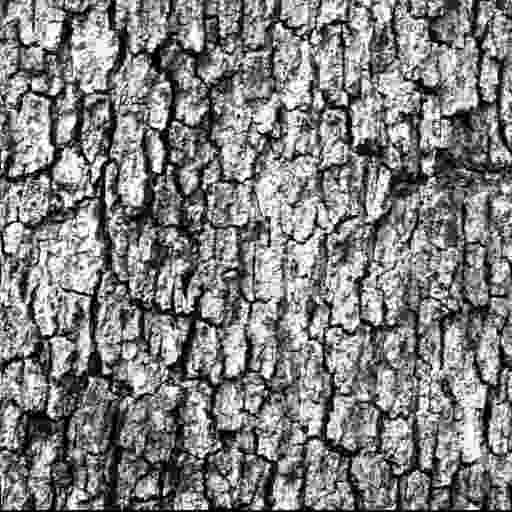
\includegraphics[width=0.3\textwidth]{../../source/Custom/pino_Q800_Custom.png} 
    \hfill 
    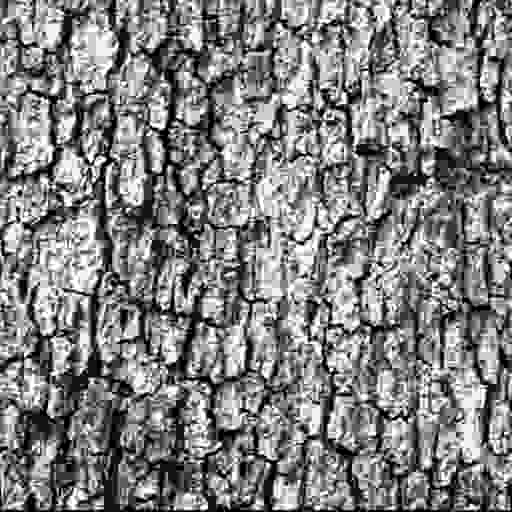
\includegraphics[width=0.3\textwidth]{../../source/Custom/pino_Q1600_Custom.png} 
    \captionof{figure}{Pino: Comparativa visual con calidades: 400, 800 y 1600 (caliQ).} 
\end{center} 
\vspace{0.5cm}

\subsubsection*{Análisis Cualitativo Pino}

\begin{itemize}
    \item \textbf{caliQ = 100}: La imagen mantiene su nitidez; no se perciben diferencias relevantes respecto a la original.
    \item \textbf{caliQ = 200}: La imagen mantiene su nitidez; no se perciben diferencias relevantes respecto a la original.
    \item \textbf{caliQ = 400}: La imagen mantiene su nitidez; no se perciben diferencias relevantes respecto a la original.
    \item \textbf{caliQ = 800}: La imagen comienza a verse levemente borrosa.
    \item \textbf{caliQ = 1600}: La imagen se percibe claramente borrosa; al ampliar la imagen se detecta un fenómeno similar al observado en Brassica para caliQ $1600$.
\end{itemize}
\subsubsection*{Análisis Cuantitativo Pino}

Esta imagen es un caso especial, ya que está en blanco y negro (escala de grises). Por ello puede representarse y almacenarse utilizando únicamente la componente de luminancia.

Como comprobación, se ha cuantificado anulando todos los coeficientes correspondientes a las componentes de crominancia, obteniéndose efectivamente la imagen original sin cambios, lo que confirma que únicamente se utiliza la dimensión de luminancia.

Para esta imagen se ha obtenido un error cuadrático medio similar al de las imágenes anteriores, aunque, al tratarse de una imagen en escala de grises, consideramos que este valor es relativamente alto.

La relación de compresión ha sido razonablemente buena, alcanzando valores cercanos al $0.7\%$ en los primeros niveles de compresión y mejorando progresivamente al aumentar el factor de cuantificación.

\begin{center}
    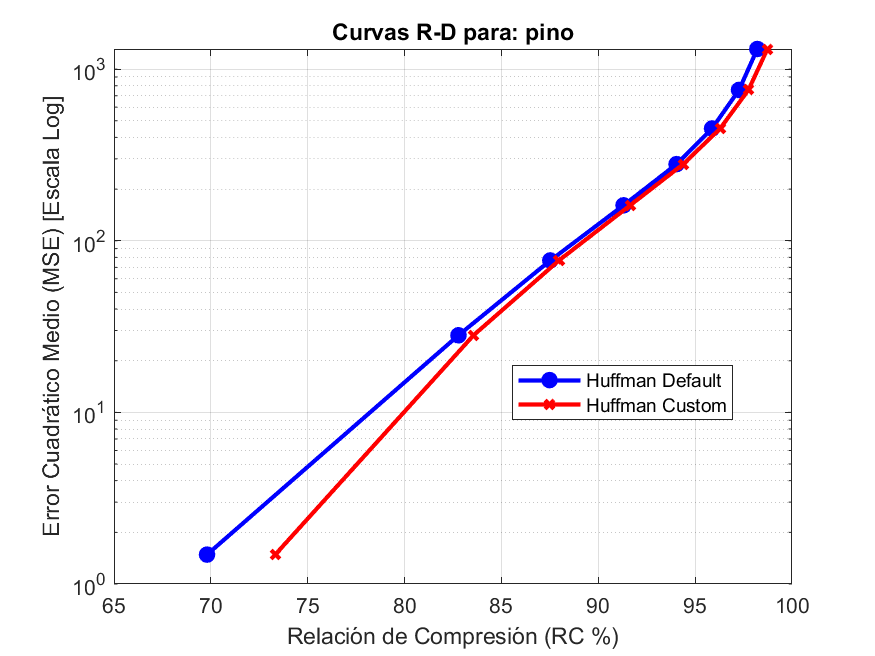
\includegraphics[width=1\textwidth]{../../source/Graficas/Grafica_pino.png}
    \captionof{figure}{pino: MSE vs RC (\%) en Escala Semilogarítmica.}
\end{center}
\vspace{0.5cm}


\begin{table}[h]
\centering
\csvautotabular{../../source/Results/pino.csv}
\caption{Resultados Pino}
\label{tab:pino}
\end{table}
\vspace{0.5cm}



\subsubsection*{Conclusión Pino}
El objetivo de esta imagen era analizar el comportamiento del compresor en un caso que requiere una cuantificación baja de los coeficientes de alta frecuencia y comprobar si se mantenía la sensación de rugosidad y nitidez.
El resultado obtenido ha sido bueno visualmente pero medio y respecto al error MSE.




\subsection{Estudio sobre los efectos de la varianza}

\subsubsection*{Introducción}
El objetivo de este análisis era comprobar si la varianza de la imagen afectaba al tiempo de compresión, así como estudiar los resultados obtenidos en relación con las dimensiones de la imagen.

\begin{center}
    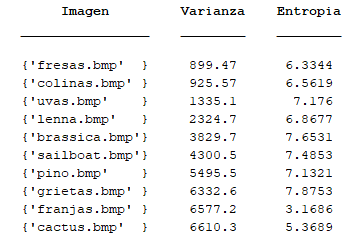
\includegraphics[width=0.7\textwidth]{./Images/estudioImagenes.png}
\end{center}
\vspace{0.5cm}

Para poder llevar a cabo este análisis, era necesario disponer de imágenes de distinto tamaño manteniendo un nivel de varianza constante en cada dimensión. Por ejemplo, si una imagen de $512 \times 512$ presenta una varianza de $4000$, una imagen de $1024 \times 1024$ debería mantener igualmente una varianza de $4000$.


\begin{center}
    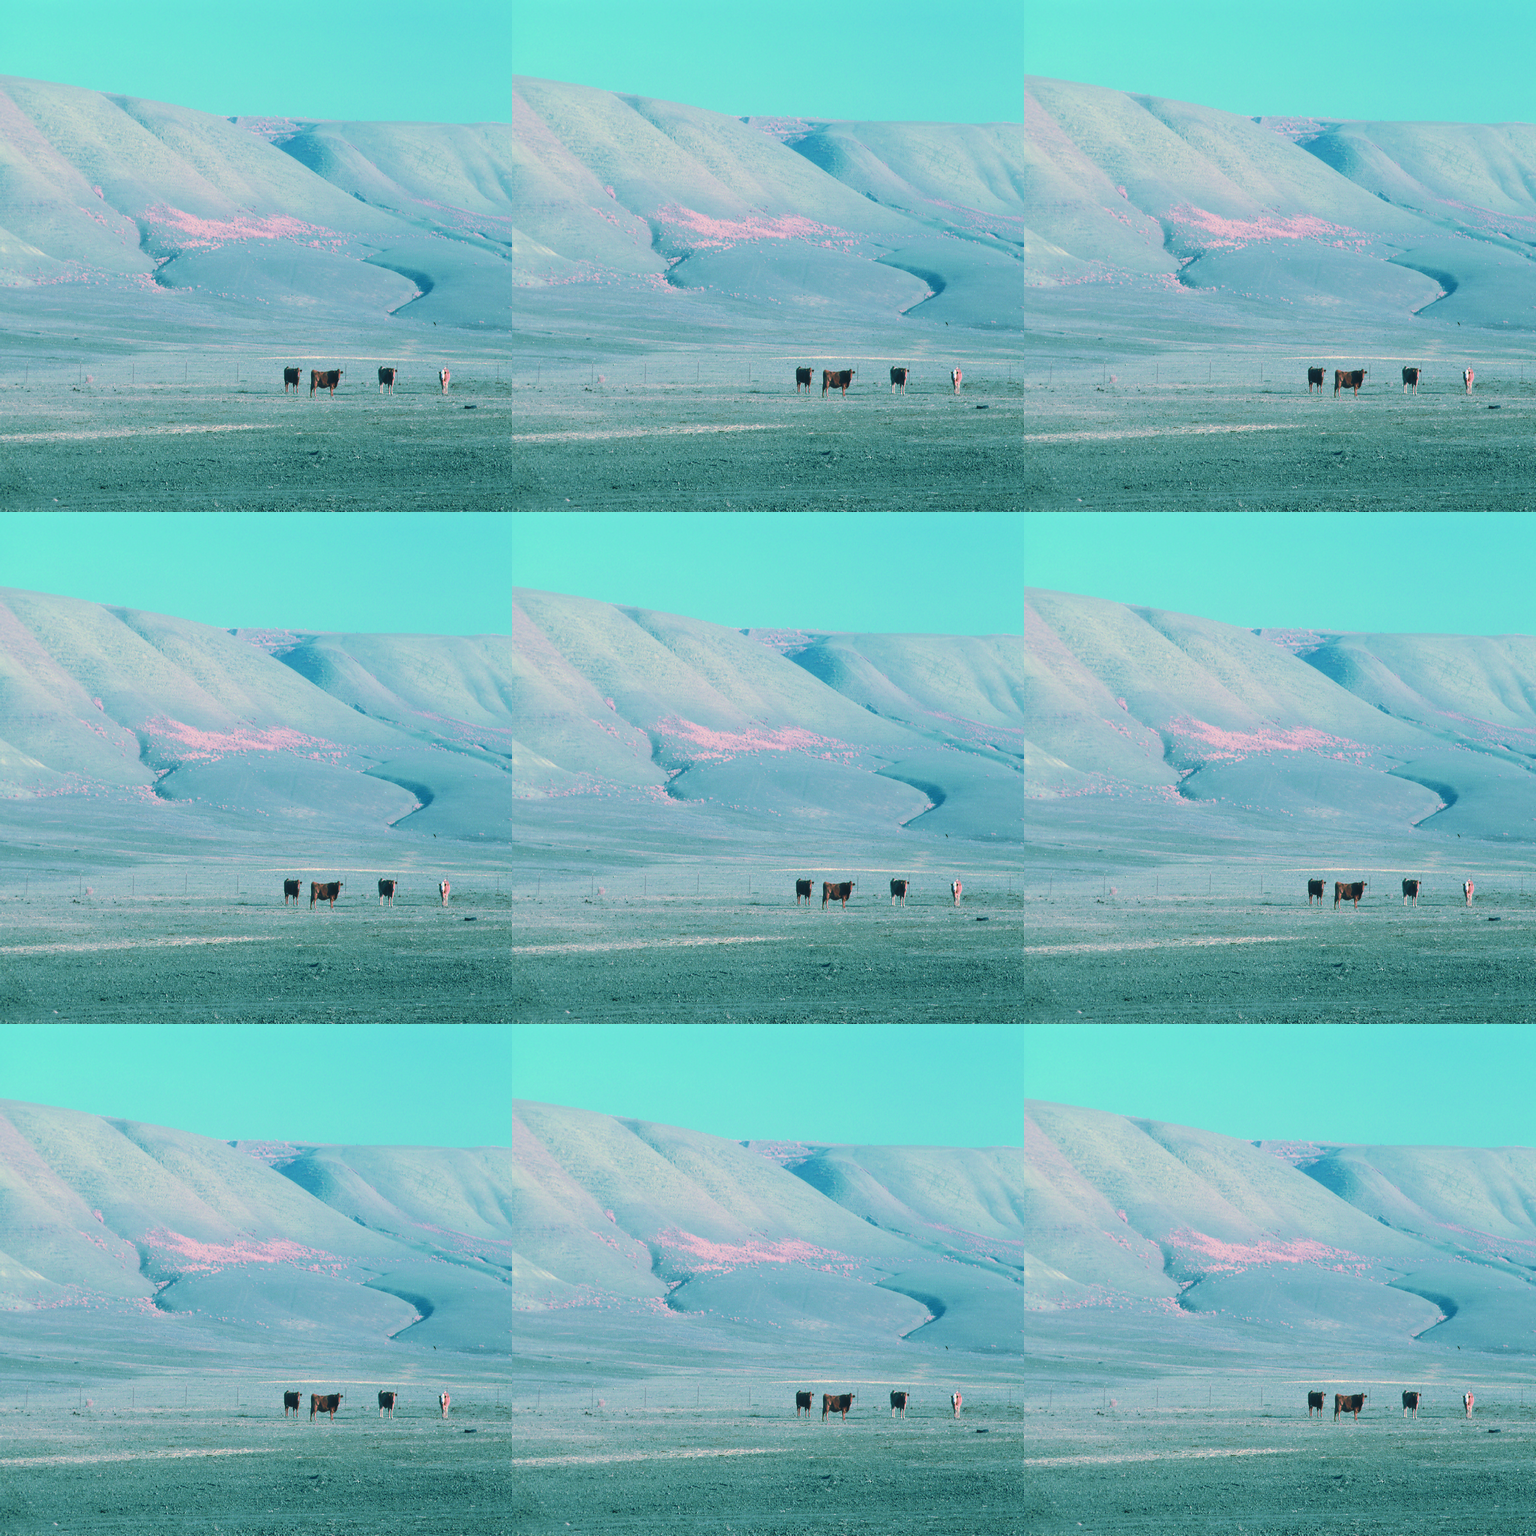
\includegraphics[width=0.8\textwidth]{./Images/colinas9x9.png}
\end{center}
\vspace{0.5cm}

\[
[512, 1024, 1536, 2048, 3072]
\]

\subsubsection*{Resultados obtenidos}
El gráfico muestra el Tiempo de Compresión (en segundos) en función del Tamaño de la Imagen (en píxeles, $N \times N$) para diez imágenes de prueba, agrupadas según su nivel de Varianza (Baja, Media y Alta) bajo una Calidad $Q=100$.

Una observación relevante es que la \textbf{varianza no ha resultado ser un indicador fiable del tiempo de compresión}. Aunque cabría esperar que las imágenes con mayor varianza presentaran tiempos más elevados, los resultados muestran varias contradicciones claras. Por ejemplo, la imagen \textit{Franjas}, clasificada con \textbf{alta varianza}, ha sido consistentemente una de las que menos tiempo ha tardado en comprimirse. En contraste, \textit{Brassica}, cuya varianza no era especialmente alta, ha resultado ser la imagen que más tiempo ha requerido, destacándose con una diferencia notable frente al resto.




\begin{center}
    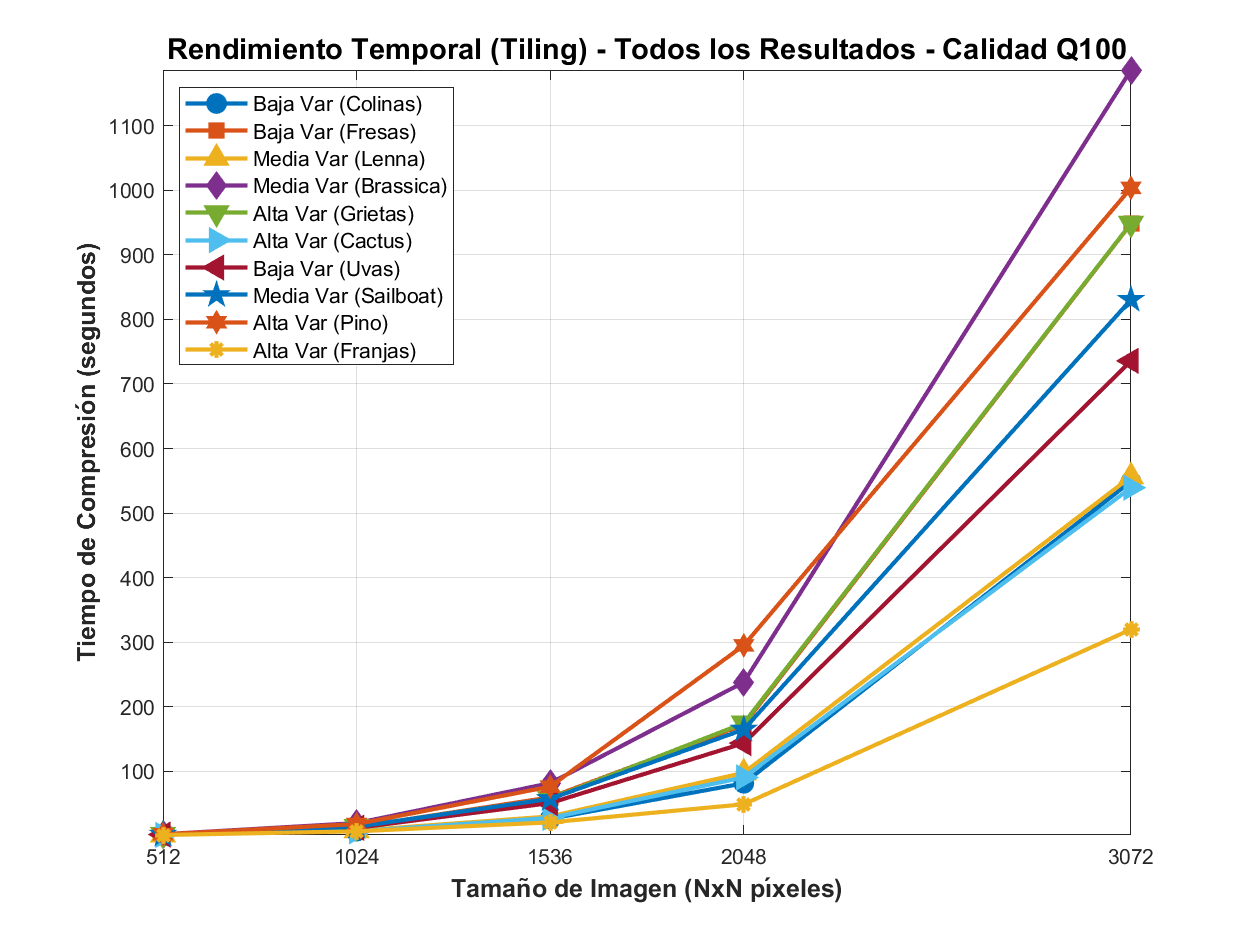
\includegraphics[width=0.8\textwidth]{../../source/Tiling_Results/Combinado_Todos.png}
\end{center}
\vspace{0.5cm}

\begin{itemize}
    \item \textbf{Tendencia Principal:}  
    La gráfica muestra claramente que el tamaño de la imagen es el factor dominante en el tiempo de compresión. El comportamiento no es lineal, sino \textbf{acelerado}, evidenciando un crecimiento que se aproxima a lo exponencial. A partir de un umbral cercano a los \textbf{2048×2048 píxeles} se aprecia un punto de inflexión donde el incremento del tiempo se vuelve mucho más pronunciado.

    \item \textbf{Eficiencia en Tamaños Pequeños:}  
    El tiempo requerido para comprimir imágenes de baja resolución varía muy poco; la diferencia entre \textbf{512×512} y \textbf{1024×1024} es mínima. Esto indica que el algoritmo mantiene una alta eficiencia en tamaños pequeños, con un coste computacional reducido y estable en esta región.
\end{itemize}

\clearpage
\begin{center}
    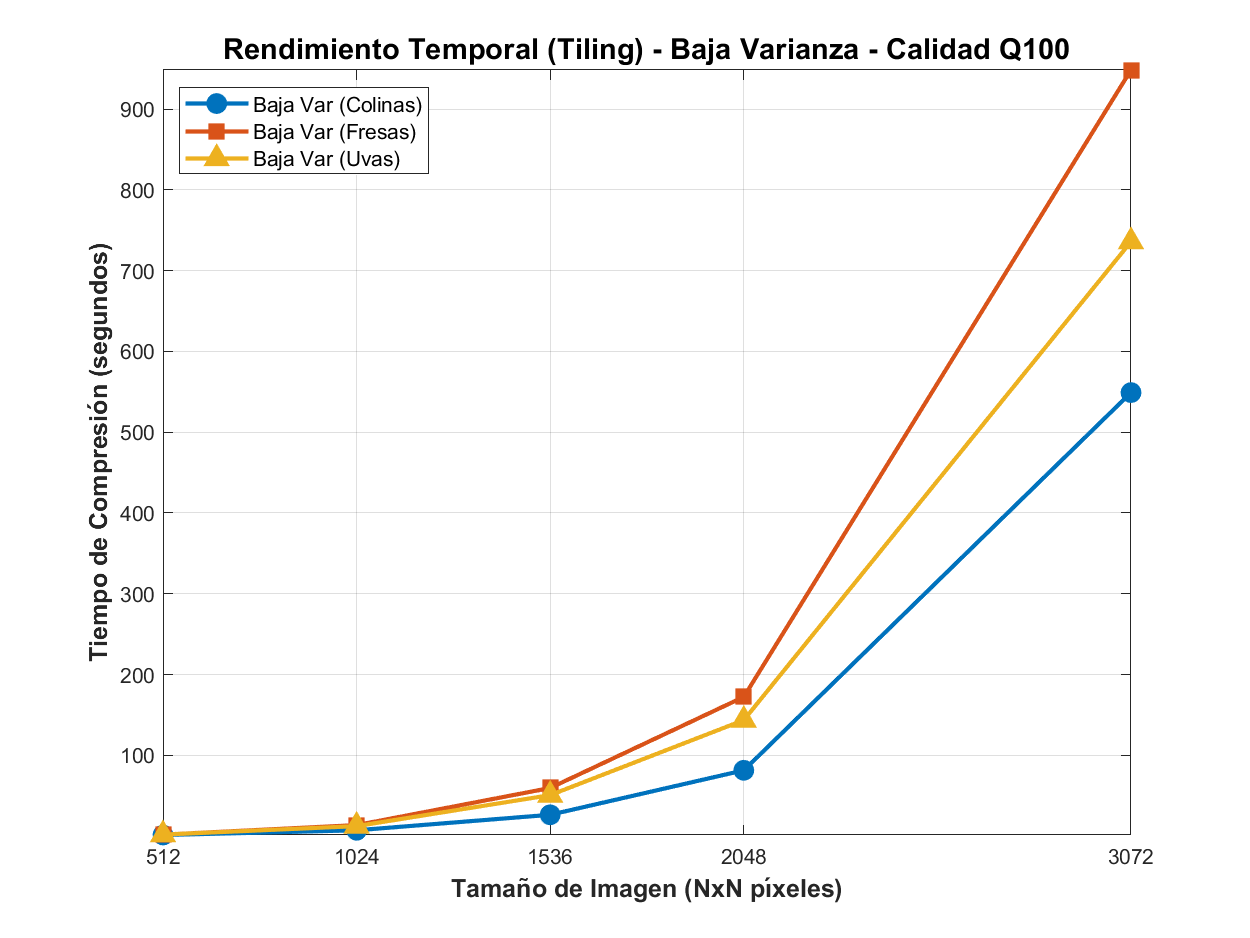
\includegraphics[width=0.65\textwidth]{../../source/Tiling_Results/Baja_Varianza.png}
    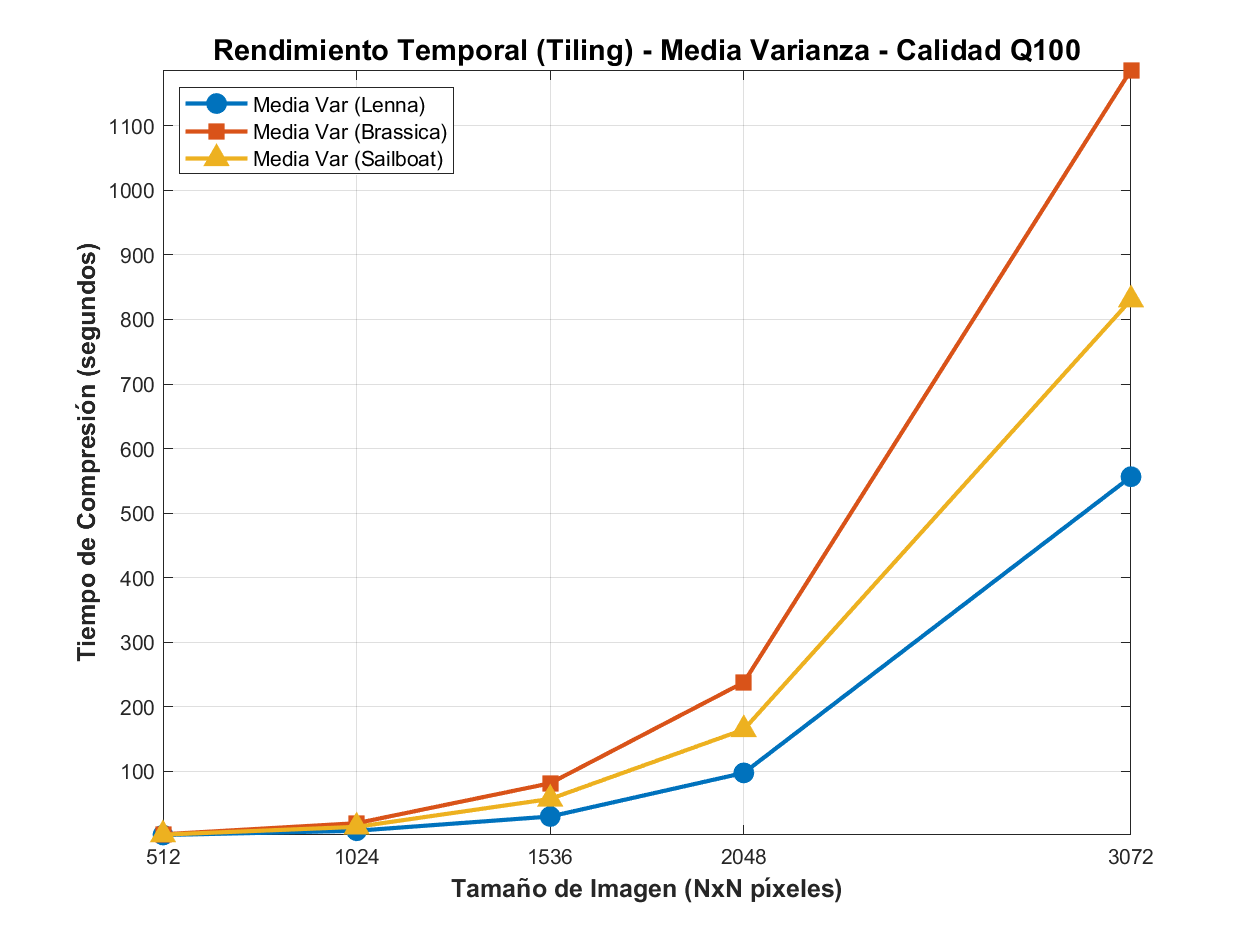
\includegraphics[width=0.65\textwidth]{../../source/Tiling_Results/Media_Varianza.png}
    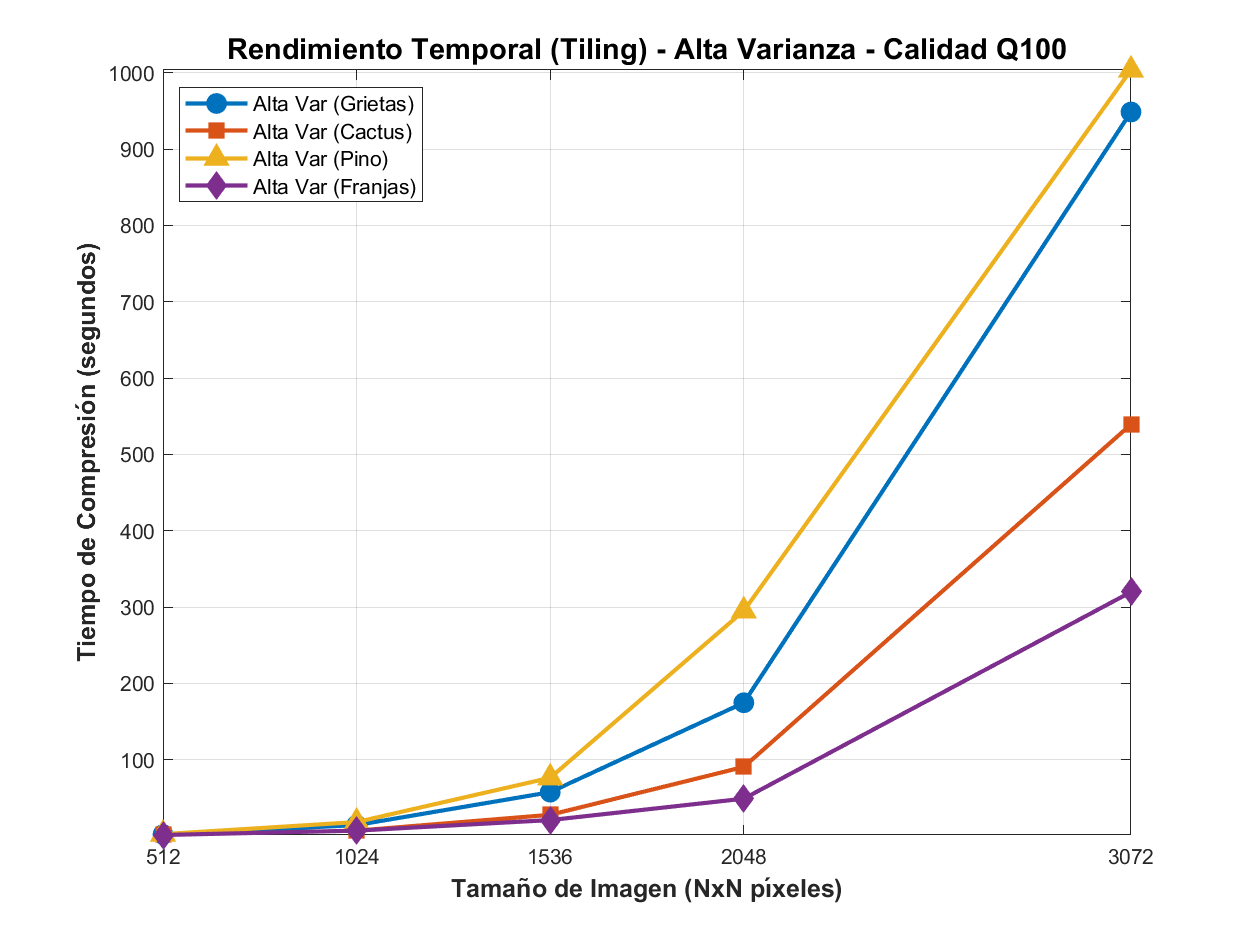
\includegraphics[width=0.65\textwidth]{../../source/Tiling_Results/Alta_Varianza.png}
\end{center}


\subsubsection*{Conclusión sobre el estudio de la varianza}
Estos resultados evidencian que la varianza, considerada de forma aislada, no es un predictor sólido del coste computacional de la compresión. El comportamiento individual de cada imagen y la distribución específica de sus patrones de píxeles tienen un impacto mucho más determinante que la mera magnitud de la varianza global.


\subsection{Codificación zonal}
En esta sección se aborda la compresión y codificación zonal mediante un estudio visual y lo más objetivo posible. Se analizará cómo la división por zonas y la selección de coeficientes influyen en la calidad reconstruida

El estudio se ha realizado para una mascara fija de $5$ coeficientes para las dimensiones de color y $5$ tamaños de zona de la dimensión de luminancia: 
\[
[5, 7, 10, 15, 20]
\]


He seleccionado una imagen representativa de cada grupo siguiendo el criterio del error cuadrático medio —bajo, medio y alto—. En el análisis nos centraremos principalmente en el resultado visual, dejando en segundo plano el tamaño final, ya que en esta prueba no se ha aplicado la cuantificación por factor CaliQ ni la matriz de pesos del estándar JPEG. En su lugar, se emplea un truncamiento de coeficientes (Codificación Zonal), una forma de cuantificación


\begin{center} 
    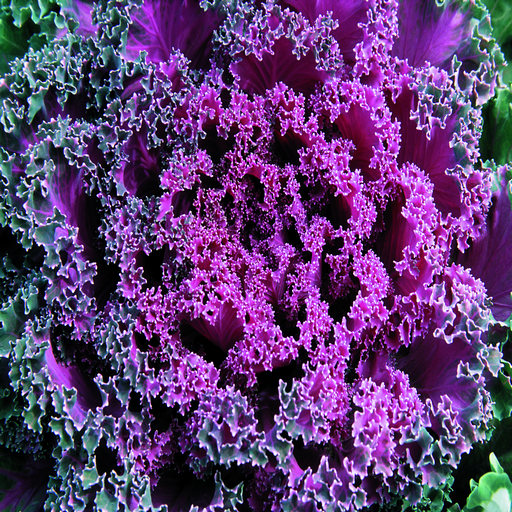
\includegraphics[width=0.3\textwidth]{./Images/brassica.png} 
    \hfill 
    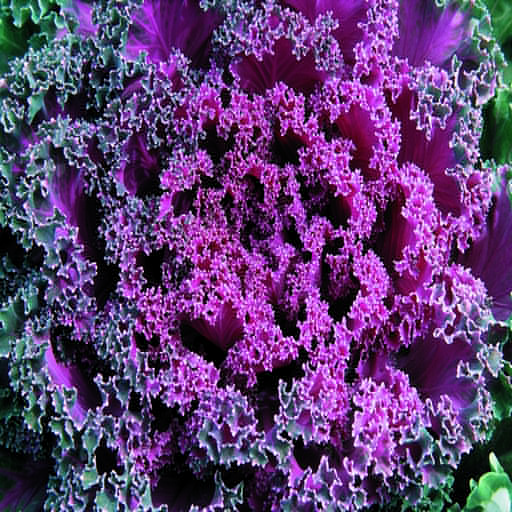
\includegraphics[width=0.3\textwidth]{../../source/Zonal/Custom/brassica_Q20_Custom.png} 
    \hfill 
    
\includegraphics[width=0.3\textwidth]{../../source/Zonal/Custom/brassica_Q15_Custom.png} 


    \captionof{figure}{Brassica: Codificación zonal con calidades: original, 20 y 15 coeficientes.} 
\end{center} 
\vspace{0.5cm} 

\begin{center} 
    
\includegraphics[width=0.3\textwidth]{../../source/Zonal/Custom/brassica_Q10_Custom.png} 
    \hfill
    
\includegraphics[width=0.3\textwidth]{../../source/Zonal/Custom/brassica_Q7_Custom.png} 
    \hfill 
    
\includegraphics[width=0.3\textwidth]{../../source/Zonal/Custom/brassica_Q5_Custom.png} 
    \hfill 

    \captionof{figure}{Brassica: Codificación zonal con calidades: 10, 7 y 5 coeficientes.} 
\end{center} 
\vspace{0.5cm}

\begin{center} 
    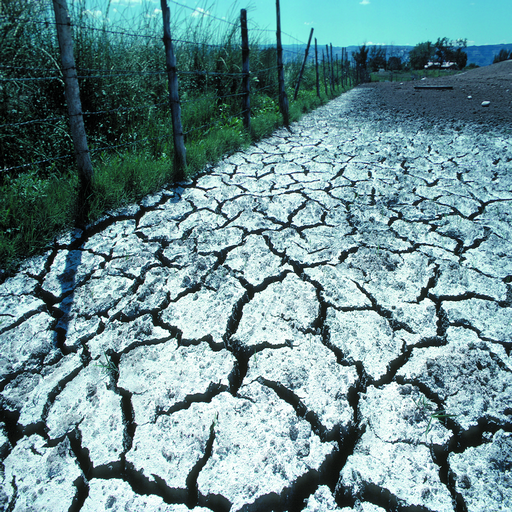
\includegraphics[width=0.3\textwidth]{./Images/grietas.png} 
    \hfill 
    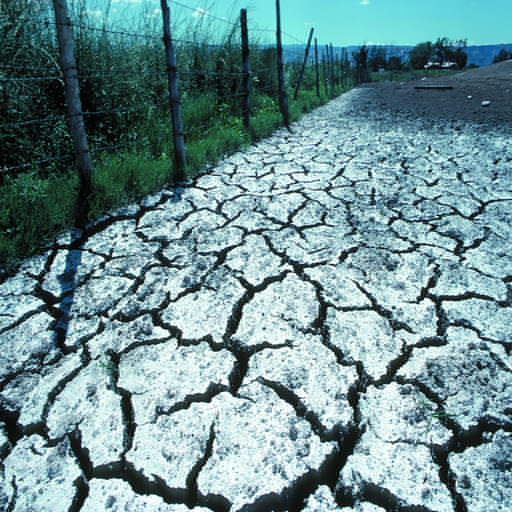
\includegraphics[width=0.3\textwidth]{../../source/Zonal/Custom/grietas_Q20_Custom.png} 
        \hfill 
    \hfill 
    
\includegraphics[width=0.3\textwidth]{../../source/Zonal/Custom/grietas_Q15_Custom.png} 
    \hfill 


    \captionof{figure}{Grietas: Codificación zonal con calidades: original, 20 y 15 coeficientes.} 
\end{center} 
\vspace{0.5cm} 

\begin{center} 
    
\includegraphics[width=0.3\textwidth]{../../source/Zonal/Custom/grietas_Q10_Custom.png} 
    \hfill 
    
\includegraphics[width=0.3\textwidth]{../../source/Zonal/Custom/grietas_Q7_Custom.png} 
    \hfill 
    
\includegraphics[width=0.3\textwidth]{../../source/Zonal/Custom/grietas_Q5_Custom.png} 

    \captionof{figure}{Grietas: Codificación zonal con calidades: 10, 7 y 5 coeficientes.} 
\end{center} 
\vspace{0.5cm}

\begin{center} 
    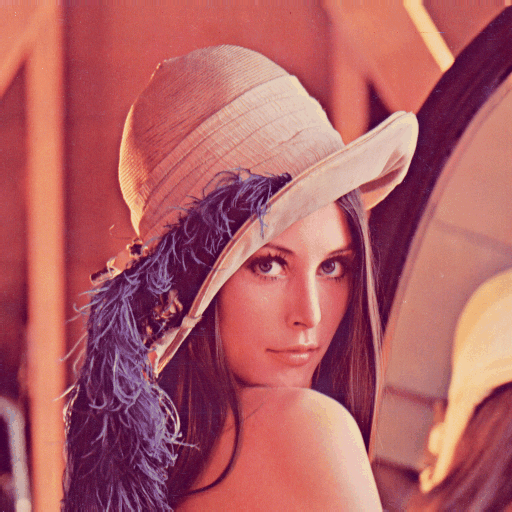
\includegraphics[width=0.3\textwidth]{./Images/lenna.png} 
    \hfill 
    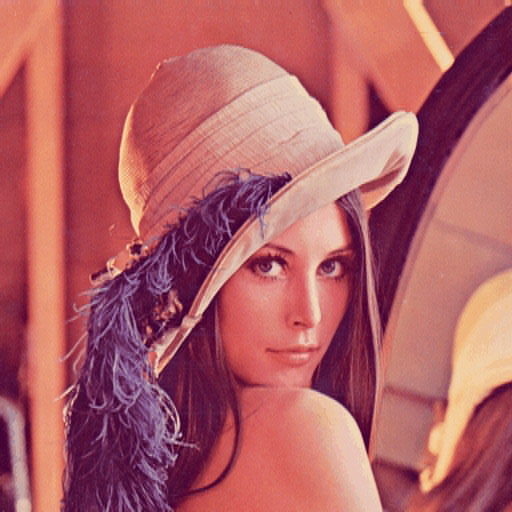
\includegraphics[width=0.3\textwidth]{../../source/Zonal/Custom/lenna_Q20_Custom.png} 
        \hfill 
    
\includegraphics[width=0.3\textwidth]{../../source/Zonal/Custom/lenna_Q15_Custom.png} 
        \hfill 


    \captionof{figure}{Lenna: Codificación zonal con calidades: original, 20 y 15 coeficientes.} 
\end{center} 
\vspace{0.5cm} 

\begin{center} 
    
\includegraphics[width=0.3\textwidth]{../../source/Zonal/Custom/lenna_Q10_Custom.png} 
    \hfill 
    
\includegraphics[width=0.3\textwidth]{../../source/Zonal/Custom/lenna_Q7_Custom.png} 
    \hfill 
    
\includegraphics[width=0.3\textwidth]{../../source/Zonal/Custom/lenna_Q5_Custom.png} 

    \captionof{figure}{Lenna: Codificación zonal con calidades: 10, 7 y 5 coeficientes.} 
\end{center} 
\vspace{0.5cm}

Los cambios o fallos introducidos al conservar $20$ y $15$ coeficientes de mayor varianza son imperceptibles en comparación con la imagen original. Al conservar únicamente $10$ coeficientes, la imagen presenta una ligera borrosidad o una leve pérdida de nitidez.

Según los resultados obtenidos, la primera observación es que seleccionar únicamente los cinco coeficientes con mayor varianza en las dimensiones de crominancia constituye una estrategia adecuada para la cuantificación de la imagen, ya que no se aprecian anomalías visuales. La segunda observación es que, en aquellas imágenes en las que el compresor presentaba un mal comportamiento al utilizar las tablas de cuantificación, este método no ha sido capaz de corregir dichos fallos.



\subsubsection*{Análisis cuantitativo}
En la imagen se muestran los resultados de aplicar cuantificación zonal para el compresor \textit{default} y el compresor \textit{custom}. Dado que la única compresión aplicada consiste en anular los coeficientes no seleccionados por la máscara, la tasa de compresión obtenida no es elevada.

Este gráfico permite apreciar la ventaja del compresor \textit{custom} frente al \textit{default}, ya que en imágenes con un gran número de valores distintos, las tablas por defecto de JPEG no están diseñadas ni optimizadas para manejar correctamente conjuntos de datos tan extensos como los obtenidos.



\begin{center}
    
\includegraphics[width=0.8\textwidth]{../../source/Zonal/Graficas/Grafica_RD_Consolidada_Unica5.png}
    \captionof{figure}{Codificación Zonal 5 coeficientes: MSE vs RC (\%).}
    \label{fig:mse_rc_5_Zonal}
\end{center}
\vspace{0.5cm}

\begin{center}
    
\includegraphics[width=0.8\textwidth]{../../source/Zonal/Graficas/Grafica_RD_Consolidada_Unica15.png}
    \captionof{figure}{Codificación Zonal 15 coeficientes: MSE vs RC (\%).}
    \label{fig:mse_rc_15_mayores}
\end{center}
\vspace{0.5cm}






%--------------------------------------------------------------------------------------------

%--------------------------------------------------------------------------------------------

\subsection{Codificación por umbral N-Mayores}

En este apartado se presenta la codificación por N mayores, donde se selecciona un número distinto de coeficientes para las componentes de luminancia y un número fijo para las de color $5$ para ser concretos. Este enfoque permite ajustar la compresión según la relevancia perceptual de cada canal. A continuación se muestran los resultados obtenidos aplicando esta técnica.

Continuamos utilizando las mismas imágenes que para la codificación zonal.

\begin{center} 
    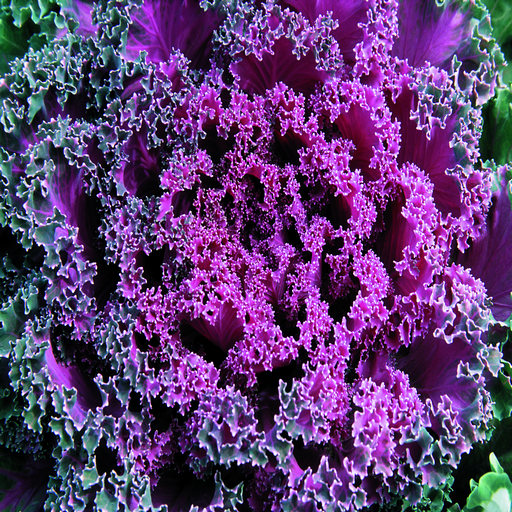
\includegraphics[width=0.3\textwidth]{./Images/brassica.png} 
    \hfill 
    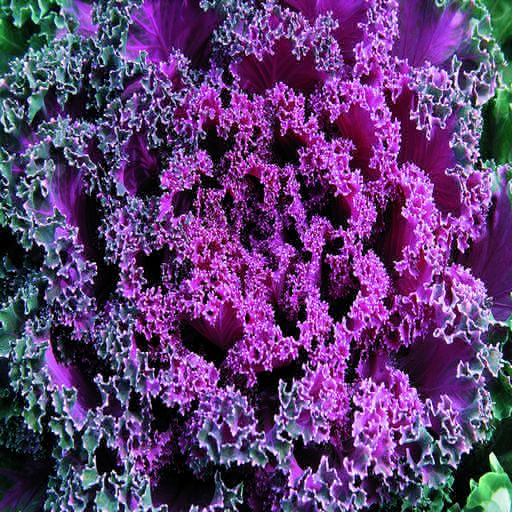
\includegraphics[width=0.3\textwidth]{../../source/Mayores/Custom/brassica_Q15_Custom.png} 
        \hfill 
    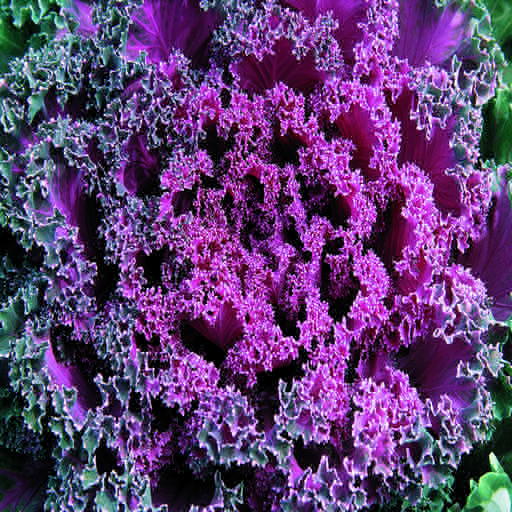
\includegraphics[width=0.3\textwidth]{../../source/Mayores/Custom/brassica_Q10_Custom.png} 


    \captionof{figure}{Brassica: Codificación zonal con calidades: original, 15 y 10 coeficientes.} 
\end{center} 
\vspace{0.5cm} 

\begin{center} 
    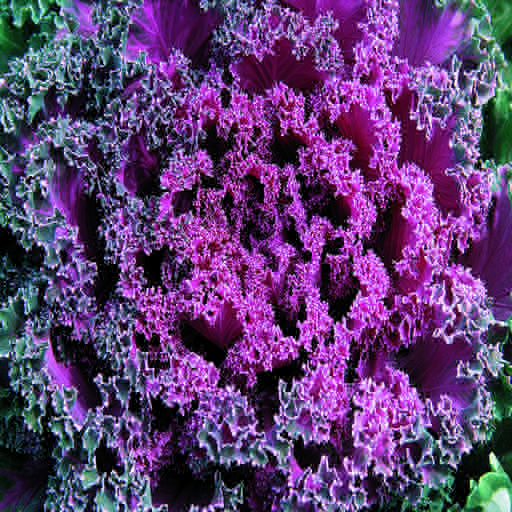
\includegraphics[width=0.3\textwidth]{../../source/Mayores/Custom/brassica_Q7_Custom.png} 
    \hfill 
    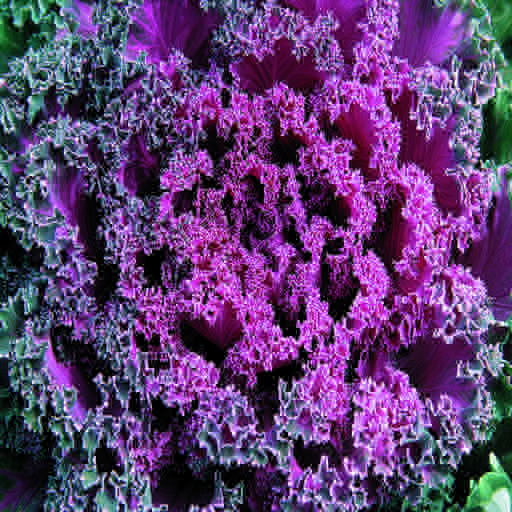
\includegraphics[width=0.3\textwidth]{../../source/Mayores/Custom/brassica_Q5_Custom.png} 
    \hfill 
    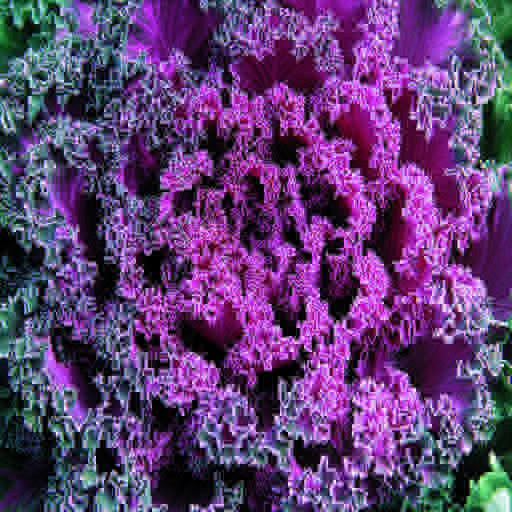
\includegraphics[width=0.3\textwidth]{../../source/Mayores/Custom/brassica_Q3_Custom.png} 

    \captionof{figure}{Brassica: Codificación zonal con calidades: 7, 5 y 3 coeficientes.} 
\end{center} 
\vspace{0.5cm}

\begin{center} 
    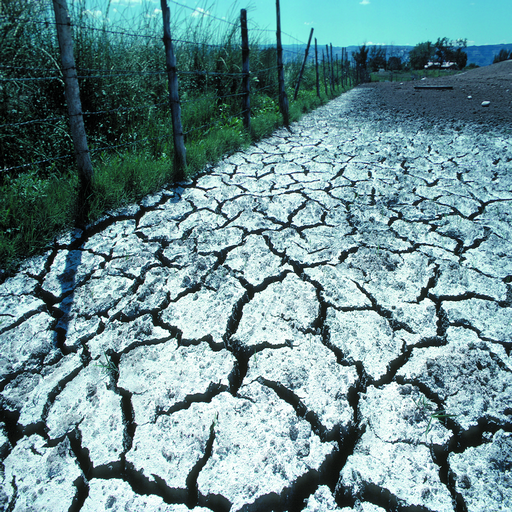
\includegraphics[width=0.3\textwidth]{./Images/grietas.png} 
    \hfill 
    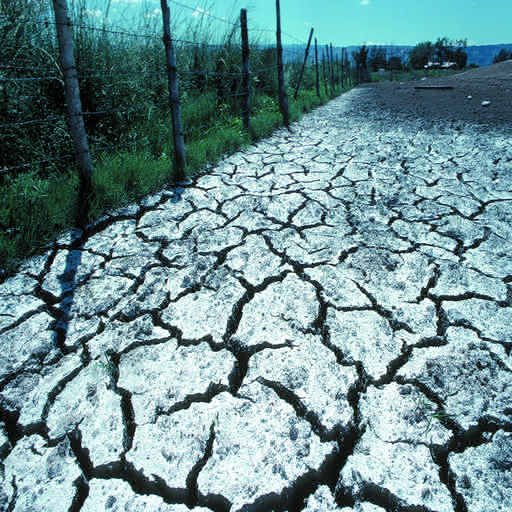
\includegraphics[width=0.3\textwidth]{../../source/Mayores/Custom/grietas_Q15_Custom.png} 
        \hfill 
    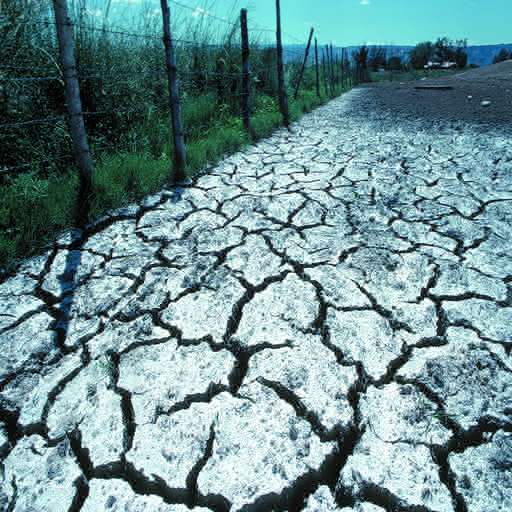
\includegraphics[width=0.3\textwidth]{../../source/Mayores/Custom/grietas_Q10_Custom.png} 


    \captionof{figure}{Grietas: Codificación zonal con calidades: original, 15 y 10 coeficientes.} 
\end{center} 
\vspace{0.5cm} 

\begin{center} 
    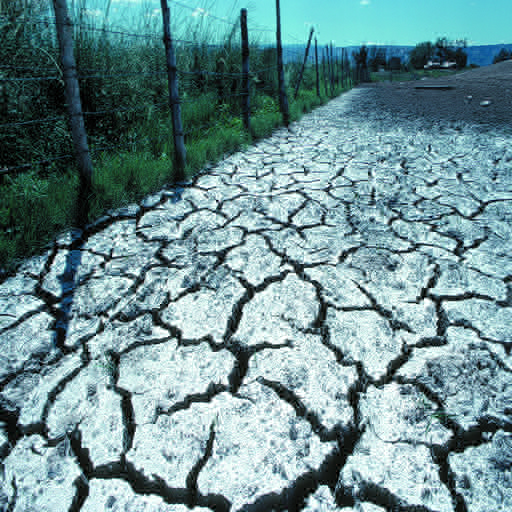
\includegraphics[width=0.3\textwidth]{../../source/Mayores/Custom/grietas_Q7_Custom.png} 
    \hfill 
    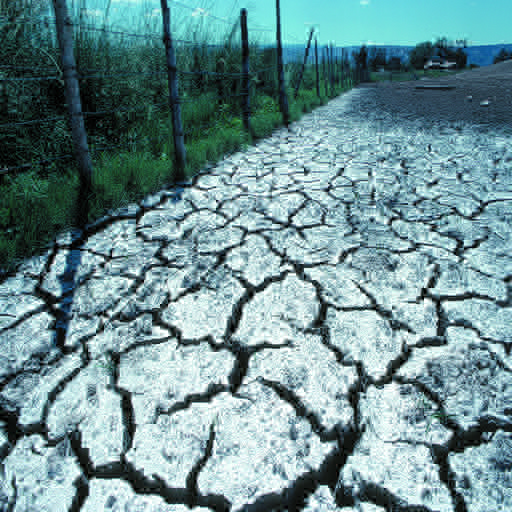
\includegraphics[width=0.3\textwidth]{../../source/Mayores/Custom/grietas_Q5_Custom.png} 
    \hfill 
    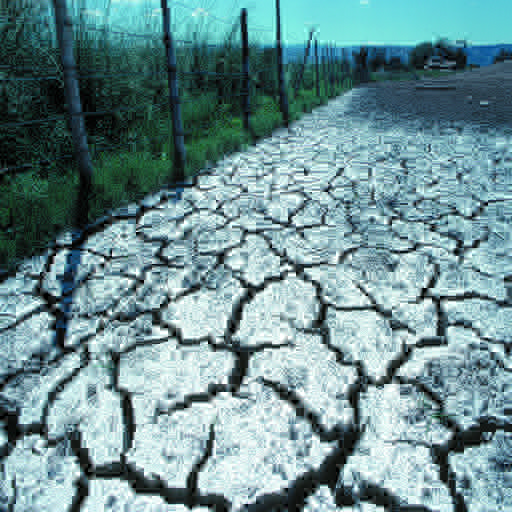
\includegraphics[width=0.3\textwidth]{../../source/Mayores/Custom/grietas_Q3_Custom.png} 

    \captionof{figure}{Grietas: Codificación zonal con calidades: 7, 5 y 3 coeficientes.} 
\end{center} 
\vspace{0.5cm}

\begin{center} 
    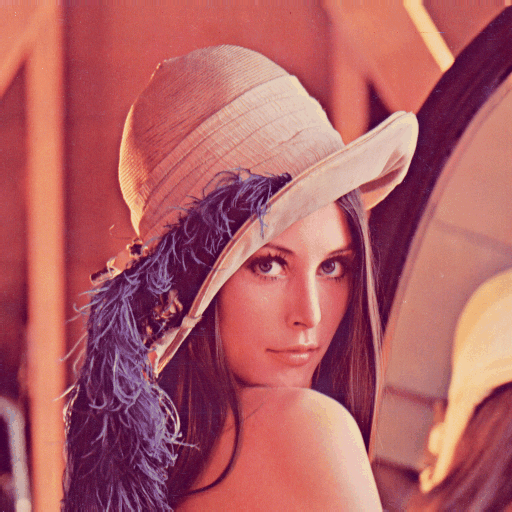
\includegraphics[width=0.3\textwidth]{./Images/lenna.png} 
    \hfill 
    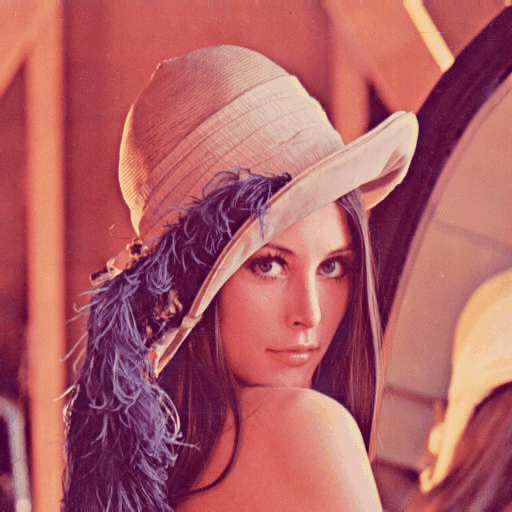
\includegraphics[width=0.3\textwidth]{../../source/Mayores/Custom/lenna_Q15_Custom.png} 
        \hfill 
    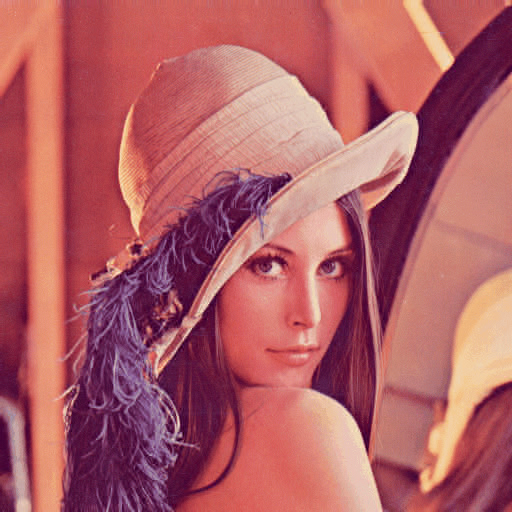
\includegraphics[width=0.3\textwidth]{../../source/Mayores/Custom/lenna_Q10_Custom.png} 


    \captionof{figure}{Lenna: Codificación zonal con calidades: original, 15 y 10 coeficientes.} 
\end{center} 
\vspace{0.5cm} 

\begin{center} 
    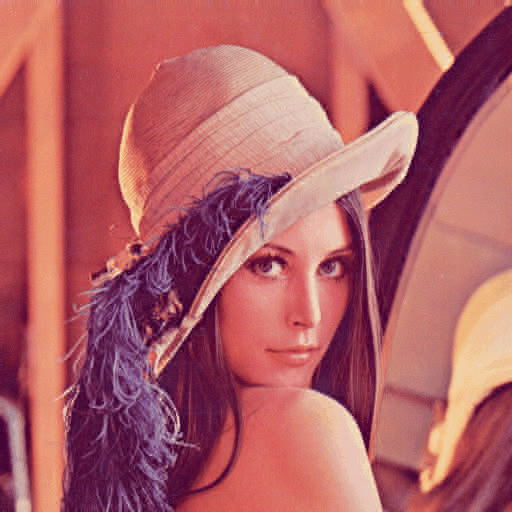
\includegraphics[width=0.3\textwidth]{../../source/Mayores/Custom/lenna_Q7_Custom.png} 
    \hfill 
    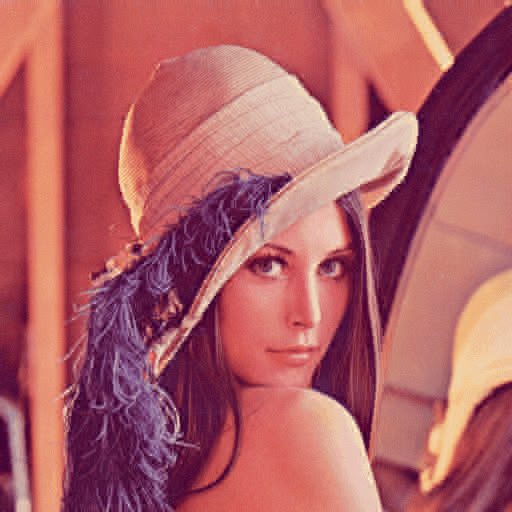
\includegraphics[width=0.3\textwidth]{../../source/Mayores/Custom/lenna_Q5_Custom.png} 
    \hfill 
    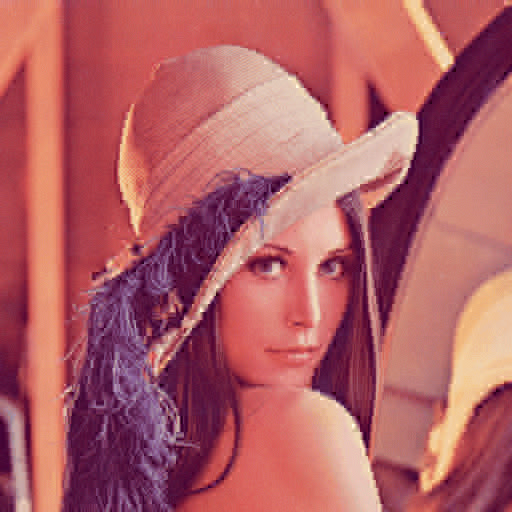
\includegraphics[width=0.3\textwidth]{../../source/Mayores/Custom/lenna_Q3_Custom.png} 

    \captionof{figure}{Lenna: Codificación zonal con calidades: 7, 5 y 3 coeficientes.} 
\end{center} 
\vspace{0.5cm}



La principal ventaja que se observa es que la forma del objeto no se pierde, sino que se conserva muy bien porque. Esto supone una clara superioridad del método, ya que con un número muy reducido de coeficientes la imagen sigue siendo identificable y mantiene una fidelidad notable respecto a la imagen original.
La desventaja principal es la perdida de nitidez e introducción de Ringing debido en gran parte a la perdida de detalles.

Seleccionar los N mayores coeficientes de una imagen es un método eficaz para la compresión, ya que —como se aprecia en las imágenes mostradas anteriormente— las versiones truncadas mantienen una gran similitud visual con las originales. No obstante, cuando se toman menos de cinco coeficientes, la reconstrucción se vuelve claramente insuficiente y los resultados dejan de ser satisfactorios.

\subsubsection*{Análisis cuantitativo}
Las siguientes tablas muestran una distribución del MSE interesante pues si comparamos el MSE de brassica lo estamos asociando a un factor CaliQ  entre 600 y 800 los efectos del truncamiento para ser menos evidentes debido a  que los defectos graves que se introducen con un factor de caliQ son muchos evidentes como pintar bloques de un solo color pero cuando utilizamos $N mayores$ ese fenómeno no ocurre.

Conservar 15 coeficientes en el caso de Brassica produce un MSE similar al obtenido con un factor de calidad $Q=400$
Aparentemente, la codificación por coeficientes resulta superior a ese factor de calidad, ya que para niveles comparables el error MSE asociado al factor CaliQ
Q es mayor.

Finalmente, para el grupo con MSE entre 0 y 250 los resultados son claramente superiores, ya que conservando únicamente 5 coeficientes se obtienen resultados comparables —no superiores, pero sí igual de buenos— a los alcanzados con un factor de calidad 
Q entre 50 y 100. Esto demuestra que ambas técnicas pueden ser efectivas cuando se aplican a imágenes adecuadas.

\begin{center}
    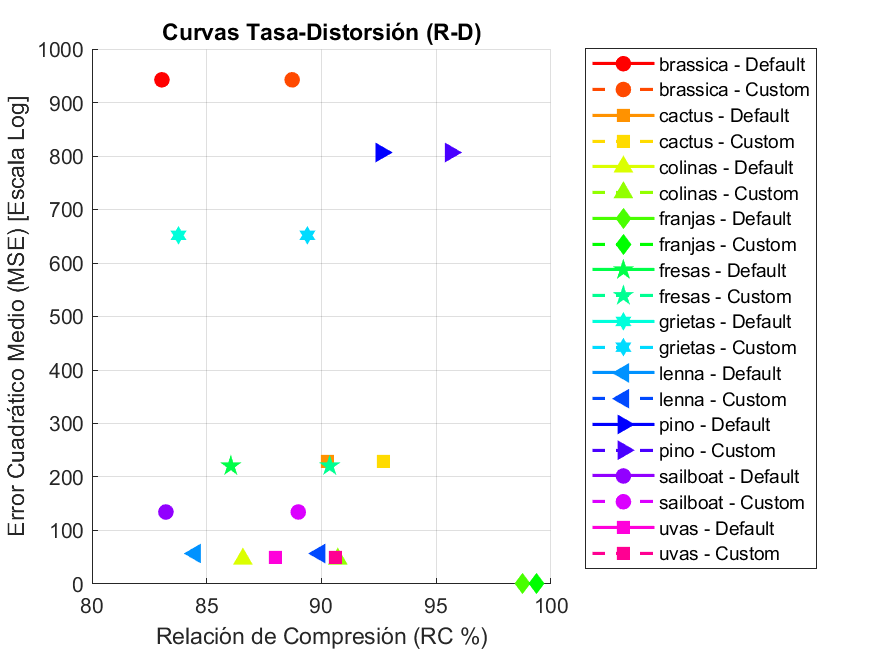
\includegraphics[width=0.8\textwidth]{../../source/Mayores/Graficas/Grafica_RD_Consolidada_Unica5.png}
    \captionof{figure}{5 mayores: MSE vs RC (\%).}
    \label{fig:mse_rc_5_mayores}
\end{center}
\vspace{0.5cm}

\begin{center}
    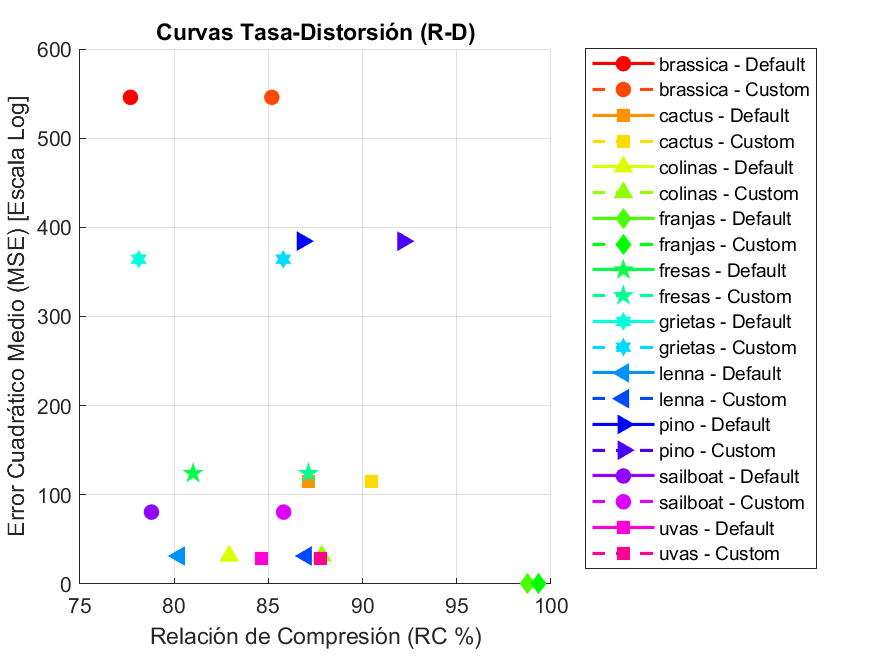
\includegraphics[width=0.8\textwidth]{../../source/Mayores/Graficas/Grafica_RD_Consolidada_Unica15.png}
    \captionof{figure}{15 mayores: MSE vs RC (\%).}
    \label{fig:mse_rc_15_mayores}
\end{center}
\vspace{0.5cm}

% --- CONCLUSIONES ---
\newpage
\section{conclusiones}

Las conclusiones derivadas del estudio experimental realizado se detallan a continuación. En primer lugar, se observa que la implementación en MATLAB opera con una eficiencia limitada, sin llegar a explotar plenamente las capacidades de hardware del equipo en el que se ejecuta.

En segundo lugar, la mejora obtenida al aplicar tablas de compresión personalizadas para cada imagen no supone un aumento significativo en la tasa de compresión. Las tablas estándar del formato JPEG funcionan correctamente, ofreciendo resultados que solo superarían a las personalizadas en casos donde el factor \texttt{caliQ} es inferior a 5 (mínima cuantización). Sin embargo, aplicar una cuantización tan baja carece de sentido práctico, ya que en ese escenario sería preferible optar por un algoritmo sin pérdida como PNG. Para factores de compresión mayores, la mejora no suele superar el 0.2\% para factores caliQ $100$, por lo que concluimos que la personalización de las tablas no es estrictamente necesaria. Sería recomendable realizar un estudio sobre los dispositivos encargados de la compresión para verificar si la relación coste-beneficio del ahorro de tamaño justifica el proceso.

En cuanto a la calidad visual, se concluye que cualquier factor de calidad por debajo de 100 introduce distorsiones mínimas o imperceptibles para el ojo humano. El factor 200 representa una frontera: algunas imágenes conservan su nitidez, mientras que otras comienzan a mostrarse ligeramente borrosas. Para un factor de \texttt{caliQ} de 400, la degradación es evidente incluso en los mejores casos, y factores superiores resultan en una calidad inaceptable con una pérdida completa de detalle.

Respecto al análisis de la varianza, se ha determinado que esta no está correlacionada directamente con el tiempo de compresión de una imagen. Según los datos obtenidos, el error cuadrático parece tener una mayor relación con el tiempo de ejecución en nuestro estudio. No obstante, es importante señalar que la muestra de imágenes seleccionada es reducida, por lo que esta afirmación dista de ser una conclusión generalizable sin un estudio más amplio.

Asimismo, se ha comprobado que mediante la selección adecuada de coeficientes, tal como se observó en el estudio zonal y de N-mayores, es posible obtener resultados satisfactorios en la reconstrucción de la imagen.

Otra de las conclusiones obtenidas es que, para aquellas imágenes en las que los compresores \textit{custom} y \textit{default} presentaban un MSE muy elevado, los compresores que emplean las técnicas de cuantificación zonal y N-Mayores no han sido capaces de resolver dichos problemas. Se concluye que este comportamiento se debe a que, en este tipo de imágenes, los coeficientes de medias y altas frecuencias tienen un peso significativamente mayor que el promedio. Por este motivo, al seleccionar un número reducido de coeficientes, el compresor obtiene resultados deficientes.

El razonamiento que sustenta esta conclusión se basa en las observaciones realizadas sobre la imagen Brassica en el estudio de cuantificación N-Mayores, donde se ha comprobado que, incluso seleccionando los diez coeficientes de mayor valor, la calidad visual se conservaba adecuadamente, mientras que al reducir el número a siete coeficientes la calidad descendía de forma notable.


En el caso de la selección de N mayores coeficientes, la conclusión es que se trata de un método menos escalable. Si se fija un número de coeficientes a conservar válido para una amplia variedad de imágenes, en muchos casos se mantienen coeficientes innecesarios; por el contrario, si se elige el número que funciona mejor para la mayoría, aquellas imágenes que requieren más coeficientes quedan fuertemente penalizadas. En comparación, el uso de tablas de cuantificación con un factor de calidad 
$Q=100$ mostró un comportamiento más equilibrado y consistente en la mayoría de las imágenes analizadas.

\section{Conclusión Personal}

Este tipo de proyectos generan en mí sentimientos encontrados. Por un lado, valoro la oportunidad de trabajar y realizar un estudio basado en mis propias hipótesis. A diferencia de otros enfoques donde se procesa un conjunto masivo de fotos para luego seleccionar los resultados más interesantes, he optado por realizar un estudio real seleccionando imágenes específicas sobre las cuales planteaba una hipótesis inicial. Hasta la finalización del estudio no se conocía la certeza de dichas suposiciones, emulando la labor de un investigador real. Espero que este enfoque justifique si, en ocasiones, los resultados pueden parecer monótonos.

Otra conclusión relevante es el redescubrimiento de la comodidad y las ventajas que aporta \LaTeX{} para la redacción de este tipo de trabajos, herramienta que no utilizaba desde el primer curso de la carrera.

Asimismo, me he propuesto realizar este trabajo utilizando únicamente los conocimientos adquiridos en la asignatura, incorporando el análisis de artefactos para comentar las imágenes con la terminología técnica adecuada. Por ello, he limitado el uso de la Inteligencia Artificial exclusivamente a la corrección ortográfica y reestructuración de textos y párrafos del documento.

Para finalizar, considero que este trabajo ha sido interesante, aunque simultáneamente tedioso debido a la repetitividad del análisis imagen por imagen sin hallar situaciones sorprendentes, las cuales seguramente existan, aunque no las haya detectado. Cabe mencionar que el proyecto se ha desarrollado en un rango de fechas complicado dentro de nuestro calendario académico.


% --- BIBLIOGRAFÍA ---
% --- BIBLIOGRAFÍA FORMAL ---
\newpage
\begin{thebibliography}{9}

    \bibitem{wiki_artefactos} Wikipedia. ``Artefactos de anillo''. Disponible en: \url{https://es.wikipedia.org/wiki/Artefactos_de_anillo} [Consultado: Diciembre 2025].
    
    \bibitem{sciencedirect_blocking} ScienceDirect. ``Blocking Artifact''. Disponible en: \url{https://www.sciencedirect.com/topics/computer-science/blocking-artifact} [Consultado: Diciembre 2025].

\end{thebibliography}

% --- RECURSOS MULTIMEDIA (IMÁGENES Y DATASETS) ---
\section*{Recursos Multimedia Utilizados}

\subsection*{Imágenes y Gráficos con URL Directa}
\begin{itemize}
    \item Gráfico 2D DCT: \url{https://www.oliviergibaru.org/courses/img/DCT_2D.png}
    \item Artefactos digitales: \url{https://matthews.sites.wfu.edu/misc/DigPhotog/alias/artifact.jpg}
    \item Color de marca (Discord): \url{https://pickcoloronline.com/es/brands/discord/colors-of-discord-512.png}
\end{itemize}

\subsection*{Imágenes de Datasets y Archivos Locales}
\begin{itemize}
    \item Imágenes de prueba (Lenna, Sailboat):
    \begin{itemize}
        \item \url{https://www.hlevkin.com/hlevkin/TestImages/lenna.bmp}
        \item \url{https://www.hlevkin.com/hlevkin/TestImages/sailboat.bmp}
        \item \url{https://sipi.usc.edu/database/database.php?volume=textures&image=15#top}
    \end{itemize}
    \item Imágenes adicionales: Obtenidas del dataset \url{https://data.mendeley.com/datasets/sp4g8h7v8k/1}
    \item Imágenes de Base64 (Códigos largos): Usadas como ejemplo en el documento.
\end{itemize}


\end{document}